\providecommand{\classoptions}{keys}
%% The next two lines are suggested at
%% to work around the following error:
%%
%%  ----------------------------
%%  /usr/local/texlive/2018/texmf-dist/tex/latex/chngcntr/chngcntr.sty:42: LaTeX Error: Command \counterwithout already defined.
%%                 Or name \end... illegal, see p.192 of the manual.
%%
%%  See the LaTeX manual or LaTeX Companion for explanation.
%%  Type  H <return>  for immediate help.
%%   ...
%%
%%   l.42 ...thout}{\@ifstar{\c@t@soutstar}{\c@t@sout}}
%%   ----------------------------
%%
%% The two lines:
\let\counterwithout\relax
\let\counterwithin\relax
%% Suggested fix above taken from
%% https://tex.stackexchange.com/questions/425600/latex-error-command-counterwithout-already-defined
%%
\documentclass[
  deliverables,
  longtasklabels,
  noworkareas,
  svgnames,
  \classoptions
]{euproposal}       % for writing
%\documentclass[submit,noworkareas,deliverables]{euproposal}        % for submission
%\documentclass[submit,public,noworkareas,deliverables]{euproposal} % for public version

\usepackage[utf8]{inputenc}
%\usepackage{minitoc}

\usepackage{float}  % used to suppress floating of tables in Resources section.
\usetikzlibrary{calc,fit,positioning,shapes,arrows,snakes}
\graphicspath{{tasks/}}

\addbibresource{bibliography.bib}
% temporary fix due to http://tex.stackexchange.com/questions/311426/bibliography-error-use-of-blxbblverbaddi-doesnt-match-its-definition-ve
\makeatletter\def\blx@maxline{77}\makeatother

%%% institutions
\WAinstitution[id=SRL,
        countryshort=NO,
        acronym=Simula]
        {Simula Research Laboratory}

\WAinstitution[id=UPSUD,
        countryshort=FR,
        acronym=UPSud]
        {Universit\'e Paris-Sud}

\WAinstitution[id=XFEL,
        countryshort=DE,
        acronym=EuXFEL]
        {European XFEL GmbH}

\WAinstitution[id=QS,
        countryshort=FR,
        acronym=QuantStack]
        {QuantStack}

\WAinstitution[id=INSERM,
        countryshort=FR,
        acronym=INSERM]
        {INSERM}

\WAinstitution[id=SIL,
        countryshort=PL,
        acronym=Silesia]
        {University of Silesia}

\WAinstitution[id=WTT,
        countryshort=CH,
        acronym=WildTree]
        {Wild Tree Tech}

\WAinstitution[id=UIO,
        countryshort=NO,
        acronym=UiO]
        {University of Oslo}

\WAinstitution[id=EGI,
        countryshort=NL,
        acronym=EGI]
        {EGI}

\WAinstitution[id=CDS,
        countryshort=FR,
        acronym=CNRS-ObAS]
        { CNRS-Observatoire astronomique de Strasbourg}

\WAinstitution[id=EP,
        countryshort=FR,
        acronym=EP]
        {\'Ecole polytechnique}



% \WAinstitution[id=PD,
%         countryshort=CH,
%         acronym=PersonalData]
%         {PersonalData.io}

\WAperson[id=minrk,
           personaltitle=Dr. ,
           birthdate=9 Oct. 1984,
           academictitle=Research Engineer,
           affiliation=SRL,
           department=Numerical Analysis and Scientific Computing,
           privaddress=None of your business,
           privtel=that neither,
           email=benjaminrk@simula.no,
           workaddress={TODO: Simula, Fornebu},
           %worktel=+33 6 77 90 32 79,
           % worktelfax=+33 6 77 90 32 79,
           %workfax=N/A
           ]
           {Benjamin Ragan-Kelley}

%%% Local Variables:
%%% mode: latex
%%% TeX-master: "proposal"
%%% End:

% LocalWords:  WAperson miko personaltitle academictitle privaddress privtel Sud
% LocalWords:  workaddress worktel workfax gc worktelfax pcg pcsa WAinstitution
% LocalWords:  shortname partof streetaddress townzip countryshort efo 3kd89
% LocalWords:  jacobs-logo.png Seefahrtstrasse Kruislann Montparnasse Universit
% LocalWords:  baz Westerfield
 % Some sections of the included files depend on this.
\usepackage{lscape} % for landscape
\usepackage{comments}
% %\usepackage[final]{comments}
\usepackage{verbatim}
\usepackage{listings}
\usepackage{supertabular,array}
\makeatletter
\newcommand\arraybslash{\let\\\@arraycr}
\makeatother
% \setlength\tabcolsep{1mm}
% \renewcommand\arraystretch{1.3}
%% Related Projects
\newcommand{\scienceproject}{\mbox{\textsc{SCIEnce}}\xspace}
\newcommand{\OOMMF}{OOMMF\xspace}
\newcommand{\OOMMFNB}{OOMMF-NB\xspace}
\newcommand{\ODK}{OpenDreamKit\xspace}
\newcommand{\VRE}{VRE\xspace}
\newcommand{\VREs}{VRE\xspace}
\newcommand{\software}[1]{{#1}\xspace}
\newcommand{\GAP}{\software{GAP}}
\newcommand{\HPCGAP}{\software{HPC-GAP}}
\newcommand{\libGAP}{\software{libGAP}}
\newcommand{\Singular}{\software{Singular}}
\newcommand{\Sage}{\software{Sage}}
\newcommand{\SageCombinat}{\software{Sage-Combinat}}
\newcommand{\MuPADCombinat}{\software{MuPAD-Combinat}}
\newcommand{\Docutils}{\software{Docutils}}
\newcommand{\Pygments}{\software{Pygments}}
\newcommand{\Sphinx}{\software{Sphinx}}
\newcommand{\SCSCP}{\software{SCSCP}}
\newcommand{\JavaScript}{\software{JavaScript}}
\newcommand{\Python}{\software{Python}}
\newcommand{\IPython}{\software{IPython}}
\newcommand{\Jupyter}{\software{Jupyter}}
\newcommand{\JupyterHub}{\software{JupyterHub}}
\newcommand{\Cython}{\software{Cython}}
\newcommand{\Pythran}{\software{Pythran}}
\newcommand{\Numpy}{\software{Numpy}}
\newcommand{\Pari}{\software{PARI}}
\newcommand{\PariGP}{\software{PARI/GP}}
\newcommand{\libpari}{\software{libpari}}
\newcommand{\GP}{\software{GP}}
\newcommand{\GPtoC}{\software{GP2C}}
\newcommand{\Linbox}{\software{LinBox}}
\newcommand{\LMFDB}{\software{LMFDB}}
\newcommand{\OpenEdX}{\software{OpenEdX}}
\newcommand{\Linux}{\software{Linux}}
\newcommand{\LATEX}{\software{\LaTeX}}
\newcommand{\SMC}{\software{SageMathCloud}}
\newcommand{\cocalc}{\software{CoCalc}}
\newcommand{\Simulagora}{\software{Simulagora}}
\newcommand{\KANT}{\software{KANT}}
\newcommand{\Magma}{\software{Magma}}
\newcommand{\Mathematica}{\software{Mathematica}}
\newcommand{\Maple}{\software{Maple}}
\newcommand{\Matlab}{\software{Matlab}}
\newcommand{\MuPAD}{\software{MuPAD}}
\newcommand{\MPIR}{\software{MPIR}}
\newcommand{\Arxiv}{\software{arXiv}}
\newcommand{\Givaro}{\software{Givaro}}
\newcommand{\fflas}{\software{fflas}}
\newcommand{\MathHub}{\software{MathHub}}
\newcommand{\FindStat}{\software{FindStat}}
\newcommand{\GitHub}{\software{GitHub}}
\newcommand{\GitLab}{\software{GitLab}}
\newcommand{\Trac}{\software{Trac}}
\newcommand{\git}{\software{git}}
\newcommand\DKS{\ensuremath{\mathcal{DKS}}\xspace}
\newcommand{\FLINT}{\software{FLINT}}
\newcommand{\nbval}{\software{nbval}}
\newcommand{\nbdime}{\software{nbdime}}
\newcommand{\nbdiff}{\software{nbdiff}}
\newcommand{\nbmerge}{\software{nbmerge}}
\newcommand{\conda}{\software{conda}}
\newcommand{\anaconda}{\software{anaconda}}
\newcommand{\clang}{\software{clang}}
\newcommand{\gcc}{\software{gcc}}
\newcommand{\cling}{\software{cling}}
\newcommand{\Julia}{\software{Julia}}
\newcommand{\Fortran}{\software{Fortran}}

%%% Local Variables:
%%% mode: latex
%%% TeX-master: "proposal"
%%% End:

\usepackage{framed}

\newcommand{\allparticipants}{{UPSUD,SRL,XFEL,QS,SIL,WTT,UIO,EGI,INSERM,CDS,EP}}

% longtaskref: T1.2: Title of task
\newcommand\longtaskref[2]{\csname task@#1@#2@label\endcsname: ``\csname task@#1@#2@title\endcsname''}

\begin{document}
\begin{proposal}[
  % These PM numbers (person months) are for the coordinator to help planning
  % Participants should not change these, but add PM numbers in the CVS in
  % the site descriptions at CVs/*.tex
  % TODO: Nicolas needs to update these numbers from the (requested ones)
  site=SRL, % Simula
  site=CDS, % CDS
  site=EP, % Ecole polytechnique
  site=EGI, % EGI
  site=XFEL, % European XFEL GmbH
  site=INSERM, % INSERM
  site=QS, % QuantStack
  site=UIO, % U Oslo
  site=UPSUD, %paris sud
  site=SIL, % U Silesia
  site=WTT, % WildTreeTech
  % site=XXX, % template example
  % alternative: (can be combined)
    coordinator=minrk,
  coordinatorsite=SRL,
  acronym={BOSSEE},
  acrolong={BOSSEE},
  proposalnumber={...},
  title=Building Open Science Services\\ on European E-infrastructure,
  callname=Topic: Prototyping innovative services,
  callid=INFRAEOSC-02-2019,
  % TODO: consistency with provided template
  % CALL: H2020-EINFRA-2015-1
  % TOPIC: e-Infrastructures for Virtual Research Environments (VRE)
  % Instrument: e-Infrastructures
  keywords={
  Open Science,
  reproducibility,
  education,
  accessibility,
  Jupyter,
  Binder,
  notebooks,
  cloud,
  EOSC,
  FAIR,
  astronomy,
  geoscience,
  health science,
  photon science,
  XFEL
  },
  % computational mathematics,
  % GAP, Linbox, PARI, Sage, Singular, IPython, Jupyter, SageMathCloud, LMFDB, MathHub
  % Virtual research environments, MPIR, /GP
  % open source, free software, number theory, abstract algebra, notebooks
  instrument= Call: INFRAEOSC-02-2019, %Call: H2020-EINFRA-2015-1, 3 Topic 9-2015
  challengeid = TODO,
  %challenge = {N/A},
  %objectiveid={N/A},
  %objective = TODO,
  %outcomeid = N/A,
  %outcome = N/A,
  months=48,
  compactht]
\newcommand{\TheProject}{\pn}% \pn is defined automatically
% \input{grantagreement-history}
\ifgrantagreement
\else
\clearpage
\TODO{In this abstract we want to summarize the vision of the project;
  - Context: Open Science; what is Jupyter; Jupyter is big
  - Who are we
  - What is our goal
  - What is our strategy / concept
Points to hit:
- Open Science should be practical, not just available
- Jupyter is part of the solution
- *brief* highlight of how/why Jupyter and Binder make sense:
  - Jupyter is widely adopted
  - notebook encapsulate computation
  - Binder builds on Jupyter to enable shareable reproducible environments
  - Jupyter is web-based, enabling building services
- What we plan to do
  - improve Jupyter/Binder toward open science
  - operate Jupyter-based services on EOSC
  - Open Science training (skip?)
- Who we are
  - Core Jupyter experts
  - Domain experts motivating/validating Jupyter improvements
}


% \begin{verbatim}
% Call: Prototyping Innovative Services for European Open Science Cloud

% Title: Building Open Science Services for European E-infrastructure (BOSSEE)

% Points to hit:

% - Open Science should be practical, not just available
% - Jupyter is part of the solution
% - *brief* highlight of how/why Jupyter and Binder make sense:
%   - Jupyter is widely adopted
%   - notebook encapsulate computation
%   - Binder builds on Jupyter to enable shareable reproducible environments
%   - Jupyter is web-based, enabling building services
% - What we plan to do
%   - improve Jupyter/Binder toward open science
%   - operate Jupyter-based services on EOSC
%   - Open Science training (skip?)
% - Who we are
%   - Core Jupyter experts
%   - Domain experts motivating/validating Jupyter improvements
% \end{verbatim}

\begin{abstract}

%  To truly achieve the societal goals of Open Science,
%  we must make progress beyond the `mere availability' of scientific results,
%  to the practical usability and exploitation of such data once it is made available,
%  an area where there is much room for improvement.
%  The Jupyter project and its ecosystem show great promise
%  as tools for bridging this gap; for making Open Science
%  useful and accessible to all,
%  from researchers to educators to public citizens.
%  The Jupyter Notebook and Jupyter ecosystem are of increasing
%  importance in computational science, data science, academia,
%  industry, governments, and service providers,
%  used by millions worldwide.
%  Jupyter notebooks have great potential to push Open Science
%  forward because they provide a complete description of a
%  computational study that can be turned into a publication
%  or produce part of a publication, such as a figure,
%  making complex tasks reproducible.
%  The Jupyter-based Binder project adds a means to execute notebooks
%  in specified computational environments, an aspect of reproducibility
%  not yet widely supported.
%  In \TheProject, we will extend the capabilities of the Jupyter
%  tools and ecosystem to add functionality that we view as having great
%  importance for EOSC and Open Science more
%  widely and operate services on EOSC as a demonstration.
%
%  Many \TheProject partners have longstanding experience and
%  leadership roles in the Jupyter ecosystem,
%  and in deploying services built on Jupyter to many users across the globe.
%  Complementary to this core expertise,
%  we integrate partners focussing on the application of these tools from a wide range of disciplines,
%  both to demonstrate and ensure that our developments serve
%  real-world Open Science use cases.
%

To truly achieve the societal goals of Open Science, we must make
progress beyond the `mere availability' of scientific results, to the
practical usability and exploitation of such data once it is made
available, an area where there is much room for improvement.  The
Jupyter project and its ecosystem show great promise as tools for
bridging this gap; for making Open Science useful and accessible to
all, from researchers to educators to public citizens.  The Jupyter
Notebook and Jupyter ecosystem are of increasing importance in
computational science, data science, academia, industry, governments,
and service providers, and used by millions worldwide.  Jupyter notebooks
have great potential to push Open Science forward because they provide
a complete description of a computational study that can be turned
into a publication or produce part of a publication, such as a figure,
thus making complex tasks reproducible. The Jupyter-based Binder project
adds a means to execute notebooks in specified computational
environments, an aspect of reproducibility not yet widely supported.

Here, we will (i) extend the capabilities of the Jupyter tools and
ecosystem to add functionality that we view as essential and providing
great value for EOSC and Open Science. Based on this framework of
improved Jupyter tools, it will be possible to Build Open Science
Services on European E-infrastructure (BOSSEE).

We will (ii) build some particular innovative EOSC open science services as
part of this project both to demonstrate and ensure that our
developments serve real-world Open Science use cases.

Many BOSSEE partners have longstanding experience and leadership
roles in the Jupyter ecosystem, and in deploying services built on
Jupyter to many users across the globe. Complementary to this core
expertise, we integrate partners focusing on the application of these
tools to a wide range of scientific disciplines and communities, for
which EOSC hosted demonstrator services are developed.

\end{abstract}

%%% Local Variables:
%%% mode: latex
%%% TeX-master: "proposal"
%%% End:

\fi
\ifsubmit\else\setcounter{tocdepth}{4}\fi
\tableofcontents

\include{outline}

% ---------------------------------------------------------------------------
%  Section 1: Excellence
% ---------------------------------------------------------------------------

\section{Excellence}
% \subsection{Context and motivation}

In many scientific disciplines, it is common for researchers to rely on
heterogeneous computational tools and technologies to collect data,
explore the input data sets, run simulations, visualise the outcome,
and share their result with peers or a with a larger audience. Often,
such data analysis cycles are iteratively refined.

For simple datasets, processes may remain manageable. However, when
dealing with larger and more complex use cases, including big data
from research facilities or High Performance Computing resources, the
complexity makes iteration cycles slower for the researchers. A
complex iteration cycle also makes research results more difficult to
reproduce.
%Results that are reproducible can much more easily be
%re-used in future work.
Results that cannot be reproduced make research ineffective: they
create barriers towards re-using the results in future research work.

This situation is exacerbated by the current and accelerating increase of the amount
of scientific data being available, including the data becoming
accessible through the EOSC-Hub. But this growing availability of data also provides a massive opportunity
for Open Science.

Project Jupyter has developed as one piece of various solutions to the data deluge,
by enabling the construction of computational services accessible from
any where, any device,
with access to any data. Jupyter-based tools such as \href{http://mybinder.org}{Binder} and repo2docker
show great promise for enabling researchers to better perform \textbf{Reproducible and Open Science}.
Jupyter was recognised for its contribution to data analysis in research with the prestigious 2017 \emph{ACM Software System Award}, of which previous winners include TCP/IP, UNIX, and the World Wide Web.
It is widely used today in research,
education, and industry.
We will build on these tools,
both improving their capabilities
and expanding their accessibility to new communities,
both academic and demographic,
in order to \textbf{further the mission of Open Science}.

In this proposal, core team members of Jupyter projects -- including a
number of recipients of the \emph{ACM Software System Award} -- and key contributors to the
open source scientific computing ecosystem,
detail improvements to the
capabilities of Project Jupyter
to \textbf{provide a framework on which innovative EOSC services can be created}.
By collaborating with a wide variety of stakeholders from diverse
science domains,
we aim to ensure and demonstrate that such
innovative EOSC services -- built on Project Jupyter -- are feasible, valuable and effective in furthering Open Science.
The goal is to \textbf{improve the
accessibility of EOSC resources to researchers and the general public,
and improve the accessibility, interactivity, reproducibility, and
re-usability of computational research
and Open Science.}


%%HF: the following seemed to be to specialised to list in the opening
%%pararaphs?
%
%which
%is especially harmful in scientific software engineering where most innovation
%is achieved through \emph{incrementalism}.




\clearpage

%%% Local Variables:
%%% mode: latex
%%% TeX-master: "proposal"
%%% End:


\subsection{Objectives}
\label{sect:objectives}
\eucommentary{1-2 pages}
\eucommentary{\emph{Describe the specific objectives for the project,
which should be clear, measurable, realistic and achievable within the
duration of the project. Objectives should be consistent with the expected
exploitation and impact of the project (see section 2).
Desirable keywords: sustainability, impact, reproducibility,
interoperability, ...
}
}
\medskip
\noindent The aims of \TheProject are to:

\begin{compactenum}[\textbf{Aim} 1:]
\item Enable a
  \textbf{sustainable}, \textbf{community-developed}, general purpose, \textbf{interoperable} toolbox for
  interactive computing, data processing, and visualization
  \textbf{that facilitates the entire life-cycle of Open Science},
  from initial exploration to \textbf{reproducible publication}, research and development in
  industry, teaching, and outreach.
  This is by supporting and steering the Jupyter software ecosystem,
  which exists to develop open source software,
  open standards, and services for interactive computing across dozens of programming languages.

\item Leverage this technology for all scientists, across borders,
  domains, disciplines, and demographics, through
  \textbf{free public distributed collaborative services} tightly integrated
  into the European Open Science Cloud (EOSC),
  in collaboration with a federation of related services
  operated by the wider community.

\item Demonstrate the value and versatility of such services through
  \textbf{innovative co-designed tailored applications} in a variety of disciplines and
  contexts.

\item \textbf{Support Open Science} and maximize impact through development and
  dissemination of best practices,
  \textbf{training}, and \textbf{community building}
  around the usage and development of the above toolbox,
  with a focus on \textbf{interoperability}, \textbf{reproducibility}
  and \textbf{reusability}.
\end{compactenum}
% develop and support the Jupyter ecosystem in a direction that benefits and facilitates open science
%     make these tools accessible to as many people as possible via operation of free, public services
%     demonstrate and ensure that these developments are useful to real scientists and the public
%     foster open science through training of students and researchers in best practices using these tools


% \item \label{aim:facilitation}
%   Facilitate Open Science through the development
%   of tools enabling reproducibility, sharing, and collaboration.

% \item \label{aim:accessibility}
%   Maximise accessibility and interoperability of Open Science services and tools,
%   across domains, disciplines, and demographics.

% \item \label{aim:sustainability}
%   Maximise sustainability of software tools for Open Science
%   by developing the community and contributing
%   to and supporting community-led software efforts.



%   Support open source software for open science, and notably the
%   Jupyter ecosystem,



% \end{compactenum}

\medskip
\noindent We will achieve our aims through the following objectives:

\begin{compactenum}[\textbf{Objective} 1:]

\item \label{obj:deployment}
  \textbf{Infrastructure and services for Jupyter on EOSC} ---
  Contribute a distributed infrastructure to the European Open Science Cloud
  (EOSC) and the wider Open Science community that can be tailored to
  provide a multitude of generic or specialized services that facilitate
  open science in a \textbf{wide range of scientific domains} and projects.
  This infrastructure will build on the Jupyter project and ecosystem,
  taking the form of a federation of JupyterHub/Binder instances,
  tightly integrated into the EOSC-Hub.
  To maximize \textbf{impact, outreach, and sustainability},
  the federation will include and encourage instances operated by
  external partners, whether free or non-free, public or private,
  general purpose or custom built for specific needs -- e.g.
  providing access to specialized or large data sets, or specific hardware.
  This objective will be supported by improvements to the Jupyter
  deployment toolbox which fosters \textbf{reuse and interoperability
    beyond the Jupyter ecosystem}.

\item \label{obj:interactivity}
  \textbf{Improving interactive computing} ---
  Improve the interactive computing capabilities of
  students, researchers, educators, and the public
  through contributions to the Jupyter environment,
  in the form of developments of interactive widgets,
  visualization tools, collaboration features, dashboards,
  teaching tools,
  and expanded support for more language communities,
  such as interactive C++.
  While Jupyter is already widely used,
  there are many areas
  of interactive exploration that can be developed further.

\item \label{obj:reusability}
  \textbf{Reproducibility and FAIR data} ---
  Extend facilities for
  \textbf{reproducibility of computational environments}
  and facilitating \textbf{FAIR data practices}.
  We will contribute to the recording and reproducibility
  of environments with repo2docker and Binder,
  and extend capabilities to better support FAIR
  data requirements. In particular, the archival of execution
  environments to support \textbf{reusability} of notebooks in the future
  needs attention. Such notebooks may, for example, be published alongside
  traditional publications to detail the computation of published data
  and figures, and address the Re-usable requirement of FAIR data.

\item \label{obj:demonstrators}
  \textbf{Demonstrators in science and education} ---
  We will demonstrate and ensure the versatility and value of the components and
  the services built from them,
  through applications to a number of
  domains in academic research, education, research infrastructures, SMEs, and for
  the public sector, driven through our project partners. In
  particular, we will contribute demonstrators in the following areas:
  astronomy (\taskref{applications}{astro}), education
  (\taskref{applications}{teaching}), fluid dynamics
  (\taskref{applications}{application-gpu}), geosciences
  (\taskref{applications}{geoscience}), health
  (\taskref{applications}{opendose-analysis}), mathematics
  (\taskref{applications}{math}),
  and photon science (\taskref{applications}{reproducibility-xfel}),
  involving universities, research infrastructure facilities, and SMEs.

\item \label{obj:outreach-and-engagement}
  \textbf{Outreach, engagement, and sustainability} ---
  Reach out to scientists and the wider Open Science and Open Data
  communities to encourage engagement
  and exploitation of the EOSC-Hub and the Jupyter-based Open Science
  Services for their research domains and interests.
  Engaging a larger community will help \textbf{ensure the sustainability} of
  the services and underlying infrastructure by distributing its
  development, hosting, and maintenance over stakeholders from a
  variety of institutions and backgrounds,
  from the private sector to public research, education
  and open government.

\end{compactenum}

\begin{table}
  \label{tab:objectives-tasks}
  \caption{
  Each objective and the tasks which further that goal.}
  \begin{tabular}{|m{.3\textwidth}|m{.7\textwidth}|}

    \hline

    \textbf{Objective} & \textbf{Tasks}
    \\\hline

    \ref{obj:deployment} &

    \longtaskref{core}{maintenance}
    \longtaskref{core}{jh-bh-conv},
    \longtaskref{eosc}{eu-binder},
    \longtaskref{eosc}{eosc},
    \longtaskref{eosc}{jh-bh-deployment}

    \\\hline

    \ref{obj:interactivity} &

    \longtaskref{core}{accessibility},
    \longtaskref{core}{collaboration},
    \longtaskref{ecosystem}{xeus-cpp},
    \longtaskref{ecosystem}{jupyter-widgets},
    \longtaskref{ecosystem}{teaching-tools}

    \\\hline

    \ref{obj:reusability} &

    \longtaskref{ecosystem}{r2d-and-binder},
    \longtaskref{ecosystem}{reproducibility}

    \\\hline

    \ref{obj:demonstrators} &
    \longtaskref{applications}{astro},
    \longtaskref{applications}{teaching},
    \longtaskref{applications}{application-gpu},
    \longtaskref{applications}{geoscience},
    \longtaskref{applications}{opendose-analysis},
    \longtaskref{applications}{math},
    \longtaskref{applications}{reproducibility-xfel}

    \\\hline

    \ref{obj:outreach-and-engagement} &

    \longtaskref{education}{workshops},
    \longtaskref{education}{online-resources},
    \longtaskref{education}{helpdesk}

    \\\hline

  \end{tabular}
\end{table}

\clearpage

\draftpage
% ---------------------------------------------------------------------------
%  Section 1.2: Relation to the work programme
% ---------------------------------------------------------------------------
% Requirements to address here:
%
% Develop an agile, fit-for-purpose and sustainable service offering
% accessible through the EOSC hub that can satisfy the evolving needs of
% the scientific community by stimulating the design and prototyping of
% novel innovative digital services. Innovative models of collaboration
% that genuinely include incentive mechanisms for a user oriented open
% science approach should be considered.

\subsection{Relation to the Work Programme}

The \TheProject project addresses the challenges of the ``Prototyping
new innovative services'' call (ID: INFRAEOSC-02-2019).

Our strategy is based on taking the increasingly popular Jupyter
Notebook and the Jupyter Ecosystem: we want to evolve and improve them
so that others can build new innovative services based of the Jupyter
tools for the EOSC.
\medskip

There is evidence that the Jupyter Notebook is an e-infrastructure
that is useful across many domains: it is already widely adopted in
numerous communities and used by millions of researchers and educators worldwide
\cite{jupyter-grant}.

\begin{itemize}
\item \emph{Journalists} and practitioners of \emph{data-driven
    journalism} at the LA Times, BuzzFeed News, Columbia Journalism School \cite{latimes-datadesk} \cite{columbia-nytimes} \cite{data-journalism},
\item \emph{Research institutions} such as CERN, JRC, and many more,
  operating institution-wide Jupyter deployment,
\item \emph{Universities} using Jupyter as a teaching platform,
\item \emph{Large cloud providers} building commercial products on the
  top of Jupyter (Google DataLab and Colaboratory, Amazon Sagemaker, Microsoft Azure
  Notebooks),
\item \emph{Other EOSC projects}. Jupyter is already planned to become
  an important service on the European Open Science Cloud (for example
  the EOSC-04-funded PaNOSC project \cite{panosc}).
\item \emph{Data scientists}: some argue that the Jupyter Notebook is
  \emph{the} tool of choice for data scientists across domains
  \cite{Perkel2018}.
\item Over 3 million notebooks are deposited on GitHub \cite{notebookcount}.
\end{itemize}
%
\begin{figure}[tb]
  \centering\includegraphics[height=0.2\textheight]{images/jeodpp.png}
  \centering\includegraphics[height=0.2\textheight]{images/jeodpp-demo.jpg}
  \caption{\emph{Left}: The Joint Research Centre (JRC) Earth Observation
    Data and Processing Platform (JEODPP) is a heavy user of the
    Jupyter Notebook (source:
    \url{https://cidportal.jrc.ec.europa.eu/home/}), where it features
    at the top of the pyramid to help users with interactive data
    visualisation and analysis. \emph{Right}: An example
    service in which an interactive visualisation is provided through
    the Jupyter notebook rendering of the density map of the ships
    detected from Sentinel-1 images over the Mediterranean sea during
    the period October 2014 to September 2016. \cite[Figure
    6]{Soille2018}. \label{fig:jeodpp}}
\end{figure}
%
A particular example is the Joint Research Centre Earth Observation
Data and Processing Platform (JEODPP) shown in Fig.~\ref{fig:jeodpp},
illustrating the interactive data exploration within an environment
that allows to save and communicate the data exploration
conveniently. These projects are building upon Jupyter as it is
available at the moment.
\bigskip

Within this context of a common software platform, we address the call
for prototyping innovative services:
\begin{itemize}
\item Our \TheProject proposal is focussed on developing the next generation
of the Jupyter tools to enable all domains to develop such services on
the EOSC.

\item Through the \TheProject-improved Jupyter, we will provide an
  agile and fit-for-purpose \emph{EOSC-enabled
framework} within which innovative services can be build by the
scientific communities.

\item We believe this is realistic as a multitude of (non-EOSC) services and
  use cases based on Jupyter have been developed, as sketched above.

\item We co-design the framework and the service demonstrators with
  core Jupyter developers, EGI and domain specialists from the
  scientific communities.

\item We will provide some particular services as part of the project
  (in the domains of astronomy, geosciences, health, mathematics, education, and photon
  science) to stimulate the design of other novel innovative services
  to address the evolving needs of the scientific community.
\end{itemize}
\bigskip


%
% % [1] EINFRAOESC-02 call (\url{https://ec.europa.eu/info/funding-tenders/opportunities/portal/screen/opportunities/topic-details/infraeosc-02-2019;freeTextSearchKeyword=innovative;typeCodes=0,1;statusCodes=31094501,31094502;programCode=null;programDivisionCode=null;focusAreaCode=null;crossCuttingPriorityCode=null;callCode=Default;sortQuery=openingDate;orderBy=asc;onlyTenders=false)}
%
% Jupyter is an important piece of infrastructure for numerous projects funded
% by the EU and its member states, including OpenDreamKit, PaNOSC, EOSC-life,
% JEODPP \cite{Soille2018}, \TODO{citations? others?}... The \TheProject project
% will thus act like a catalyst, increasing the potential impact of all these
% projects, as well as hopefully many future projects, by strengthening a common
% software platform.
%
%
%
% % Lots of EOSC and EU-funded projects are built upon jupyter
% %
% % Opendreamkit
% % PaNOSC
% % JEODPP https://www.sciencedirect.com/science/article/pii/S0167739X1730078X?via%3Dihub
% % EOSC-Pilot
% % EGI https://ec.europa.eu/info/funding-tenders/opportunities/portal/screen/opportunities/topic-details/infraeosc-02-2019;freeTextSearchKeyword=innovative;typeCodes=0,1;statusCodes=31094501,31094502;programCode=null;programDivisionCode=null;focusAreaCode=null;crossCuttingPriorityCode=null;callCode=Default;sortQuery=openingDate;orderBy=asc;onlyTenders=false
% %
% % Jupyter is a critical piece of European e-infrastructure; this project is important for sustainability, we need not just to build upon Jupyter but to consolidate the foundations.
% %
% % We also want to enable novel use cases to enable advances in European computational and data science activities that build on the Jupyter ecosystem.
% %
% % Who is better placed than the team who built Jupyter in the first place to move Jupyter forward?
% %
% % JEODPP Image (jeodpp_new_small_4.png)
% %
% %
% % The main challenge we need to address is “Develop an agile, fit-for-purpose and sustainable service offering accessible through the EOSC hub that can satisfy the evolving needs of the scientific community by stimulating the design and prototyping of novel innovative digital services. Innovative models of collaboration that genuinely include incentive mechanisms for a user oriented open science approach should be considered.” (from Specific challenge in: https://ec.europa.eu/info/funding-tenders/opportunities/portal/screen/opportunities/topic-details/infraeosc-02-2019;freeTextSearchKeyword=innovative;typeCodes=0,1;statusCodes=31094501,31094502;programCode=null;programDivisionCode=null;focusAreaCode=null;crossCuttingPriorityCode=null;callCode=Default;sortQuery=openingDate;orderBy=asc;onlyTenders=false)
% %
% % We need to make sure to either put this phrase in and respond to how we address it, or drop the right keywords.
% %
% %
% % \TODO{We should also go through the requirements from the call [1] and
% %   show how we address those [to provide easily accessible evidence
% %   that we are addressing the call].}
% %


\draftpage
% ---------------------------------------------------------------------------
%  Section 1.3: Concept and Approach
% ---------------------------------------------------------------------------
\TOWRITE{NT/...}{Finalise}
\TOWRITE{ALL}{Proofread concept and approach pass 2}

\subsection{Concept and Methodology}\label{sec:concept_methodology}
\eucommentary{5-8 pages}
\eucommentary{
-- Describe and explain the overall concept underpinning the project.
Describe the main ideas, models or assumptions involved. Identify
any trans-disciplinary considerations;
-- Describe and explain the overall approach and methodology, distinguishing, as
appropriate, activities indicated in the relevant section of the work programme, e.g.
Networking Activities, Service Activities and Joint Research Activities, as detailed in
the Part E of the Specific features for Research Infrastructures of the Horizon 2020
European Research Infrastructures (including e-Infrastructures) Work Programme 2014-
2015;\\
-- Describe how the Networking Activities will foster a culture of co-operation between the
participants and other relevant stakeholders.\\
-- Describe how the Service activities will offer access to state-of-the-art infrastructures,
high quality services, and will enable users to conduct excellent research.\\
-- Describe how the Joint Research Activities will contribute to quantitative and qualitative
improvements of the services provided by the infrastructures.\\
-- As per Part E of the Work Programme, where relevant, describe how the project will
share and use existing basic operations services (e.g. authorisation and accounting
systems, service registry, etc.) with other e-infrastructure providers and justify why such
services should be (re)developed if they already exist in other e-infrastructures. Describe
how the developed services will be discoverable on-line.\\
-- Where relevant, describe how sex and/or gender analysis is taken into account in the
project's content.}


\subsubsection{Concept}\label{sec:concept}

Open Science is the principle that science, in order to be most
impactful and socially responsible, should be done publicly, with as
much of the scientific process and products accessible, reviewable,
and reusable by as many members of the global community as possible.
In the modern age of computational science, almost all academic
fields, from humanities to social sciences to biology and astronomy
are faced with exciting opportunities for Open Science.  As more and
more research takes the form of code and/or data, the opportunity to
share, reproduce, and reuse scientific work is greater than ever, even
enabling new forms of interdisciplinary collaboration.

At the same time as we share in these exciting opportunities, there
are corresponding challenges, technical and social, to making Open
Science a practical reality.  We face big questions: If a researcher
has code and/or data to publicise, how is that best done?  How do
researchers learn best Open Science practices in their field?  How do
previously disconnected fields benefit from each other's work as the
same computational challenges are faced again and again by different
communities?

These are the questions that guide \TheProject.
With so much research being done that wants to be Open,
how can we make Open Science

\begin{enumerate}
    \item as easy as possible to share?
    \item as useful as possible to other researchers and the public?
\end{enumerate}

\noindent Our plan for improving access and effectiveness of Open Science can be summarised as:

\begin{enumerate}
\item improve and maintain common software infrastructure used for
  Open Science,
\item develop the Jupyter ecosystem to improve capabilities to better
  serve Open Science,
\item guide, validate, and demonstrate our developments through
  collaboration with a wide variety of application domains,
\item enable students and researchers to perform Open Science through
  training and education, and improving inclusiveness by focusing
  these on under-served and under-represented communities, and
\item operate services to facilitate Open Science collaborations with
  Jupyter software.
\end{enumerate}

\medskip

\subsubsection{Project Jupyter and the surrounding ecosystem}
\label{sec:project-jupyter}

\begin{figure}[htb]\centering
  \includegraphics[width=0.9\textwidth]{use-cases-binder-logbook-solution.png}
  \caption{A typical use case for Jupyter notebooks in research.
            Image by Juliette Belin for the OpenDreamKit project, used under
            CC-BY-SA.}\label{fig:use-cases-binder}
\end{figure}

\noindent\textbf{Jupyter ecosystem as the root of \TheProject}


\TheProject has chosen to centre its efforts on the Jupyter software
ecosystem. Figure~\ref{fig:use-cases-binder} summarises a typical use
case of Jupyter Notebook and Binder; both are described in more detail
below.

The Jupyter notebook and Jupyter ecosystem are of increasing
importance in computational science and data science, in academia,
industry and services. In addition to supporting high productivity of
researchers, they have great potential to push open science forward:
the notebook provides a complete description of a computational and
data science study (Step 1 in figure~\ref{fig:use-cases-binder}), and the notebook can -- in principle -- be turned
into a publication, or can be used to provide the required computation
for a part of a publication, such as a figure
(Step 2 in figure~\ref{fig:use-cases-binder}). Once the researcher has
specified what software is required to execute the notebook (Step 3
in figure~\ref{fig:use-cases-binder}), the study is completely
reproducible by anyone (Step 4 in figure~\ref{fig:use-cases-binder}).

In this way, the notebook enables reproducibility of complex tasks
with hardly any additional effort on the user side (if used
appropriately). The Binder project allows to execute such notebooks in
tailored computational environments; an aspect of reproducibility that
is not widely supported yet.

Furthermore, for users wanting to connect
to a local Jupyter notebook server on their machine, or to connect to
a server somewhere else on the Internet, the users only need a
web-browser to display and use the notebook regardless of the location
of the notebook server. Because of these
characteristics, the Notebook is already planned to become an
important service on the European Open Science Cloud (EOSC) (for
example in \cite{panosc}).

\medskip\noindent\textbf{Project Jupyter}

\emph{Project Jupyter} \cite{Jupyter}, which has grown increasingly popular in the scientific
computing community, has become the \emph{lingua franca} of interactive
computing in both academia and industry. The main goal of Project Jupyter
project is to provide a consistent set of tools to improve researchers'
workflows from the exploratory phase of the analysis to the communication
of the results \cite{Kluyver2016}.

Started in 2014 from the \emph{IPython Project} \cite{IPython}, Jupyter has grown rapidly in
popularity and adoption both in the industry and academia. We estimate the user
base of the Jupyter notebook to be in the millions. Users range from data
scientists to researchers, educators, and students from many fields,
including journalists and librarians. In 2017, the Jupyter
team was awarded the \emph{ACM Software System Award}, an annual award that
honors people or an organization \emph{"for developing a software system that had a
lasting influence"}. Prior recipients include \emph{Unix}, \emph{TCP/IP}, and
the \emph{World Wide Web} \cite{acm-award}.

A large number of discrete software components make up Project Jupyter.
While these interact with one another, many can be installed separately
to serve various use cases. For this proposal, we loosely divide the
software involved into \emph{Jupyter core} developed under the guidance
of the developers who started the project, and the broader \emph{Jupyter
ecosystem} including software developed by third parties. Some of the
important components and concepts are detailed below.

\begin{figure}[ht]\centering
  \centering
  \includegraphics[width=0.9\textwidth]{spectrogram_smaller.png}
  \caption{A notebook document in the Jupyter Notebook interface.}\label{fig:notebook-screenshot}
\end{figure}

\medskip\noindent\emph{Jupyter core}
\begin{itemize}
  \item The \textbf{Jupyter Notebook} is the flagship application of Project Jupyter.
  It allows the creation of notebook documents, containing a mixture of text and
  interactively executable code, along with rich output from running that code.
  Figure \ref{fig:notebook-screenshot} shows an open notebook including graphs
  from an audio processing example. Notebook documents are readily shareable,
  providing a popular way to describe and illustrate computational methods and
  tools.
  \textbf{JupyterLab} is the new, modular, extensible client application
  for Jupyter notebooks.

  \item \textbf{Jupyter kernels} are the backend software which allow Jupyter to execute
  code in many different programming languages. The \textbf{IPython} kernel is
  the reference kernel, supporting the Python programming language, and is
  developed by the Jupyter core team. Kernels for other languages are maintained
  by third parties.

  \item \textbf{nbconvert} converts notebook files to a variety of other file
  formats, including HTML and PDF, so that the content of a notebook can easily
  be shared with people who don't have Jupyter software. nbconvert also powers
  \textbf{nbviewer}, a web service which provides static HTML views of publicly
  accessible notebooks.

  \item \textbf{JupyterHub} is a multi-user extension of the Jupyter Notebook.
  It runs on one or more notebook servers, for example at a research institution.
  Users can log in to author and run notebooks securely through their web
  browser, without needing to install any special software on their own
  computer.

\end{itemize}

While Jupyter is a large, distributed, coordinated project,
the wider community of Jupyter users develops a great deal of
software with Jupyter integration,
providing increased or domain-specific functionality,
building on top of Jupyter, or integrating core Jupyter components in some aspect.
We call this the \textbf{Jupyter ecosystem}.
The broader Jupyter ecosystem includes many more projects than we will describe
here, but a selection of projects which are relevant to
\TheProject includes:

\medskip\noindent\emph{Jupyter ecosystem}\label{jupyter-ecosystem}

\begin{itemize}
  \item \textbf{Binder} builds on JupyterHub to allow sharing executable
  environments along with data files and a description of the libraries
  required to run the notebooks. When someone accesses a Binder repository,
  the service builds the computational environment on-demand, allowing them to
  execute and modify a copy of the notebooks.
  \textbf{repo2docker} \cite{repo2docker} and \textbf{BinderHub} \cite{binder} are components of the Binder
  software.

  \item \textbf{nbsphinx} \cite{Nbsphinx} integrates notebooks with the \emph{Sphinx}
  documentation system, which is widely used for software documentation,
  especially but not only for software written in Python.
  This allows developers to write notebooks showing how to use a library,
  then seamlessly make those notebooks part of their main documentation.

  \item \textbf{nbval} \cite{nbval} is a plugin for the popular \emph{pytest} testing
  framework to automatically execute notebooks and optionally check that the
  output matches that saved in the file. While this is not a subsitute for a
  test suite, it's valuable for documentation with code examples in notebooks.
  If changes to the underlying tools mean the example no longer
  works, testing with nbval will quickly show this, so that either the software
  or the example can be corrected. This ensures that example code and
  documentation don't get outdated.

  \item \textbf{nbdime} \cite{nbdime} provides tools for comparing and merging notebooks.
  These integrate with version control systems such as \emph{git}, which
  are designed for plain text files and typically don't handle notebook files
  well.

  \item \textbf{Widgets} allow interactive output in the notebook which can
  communicate with the kernel, updating values in the kernel and updating the
  displayed output as code runs. \textbf{ipywidgets} \cite{ipywidgets} provides the main
  implementation for the IPython kernel, while other packages such as
  \textbf{bqplot} \cite{bqplot}, \textbf{ipyvolume} \cite{ipyvolume} and
  \textbf{K3D} \cite{K3D} extend the framework to provide 2D and 3D visualisations.
  Figure \ref{fig:ipywidgets-example} shows a simple example of interactive
  widgets in use.

  \item The \textbf{Voila} package \cite{Voila} enables the
  sharing of notebook-based interactive dashboards for non-technical users.

  \item The \textbf{Xeus} instrastructure \cite{Corlay2017} supports writing kernels
  in C++. \textbf{xeus-cling} is one such kernel, running user code in C++,
  and built upon CERN's C++ interpreter, "cling" \cite{Vassilev2012},
  which has a lot of adoption in the High-Energy-Physics community.
  xeus-cling is already in use for teaching the C++ programming language.
\end{itemize}

\begin{figure}[ht]\centering
  \includegraphics[width=0.5\textwidth]{ipywidgets_example.png}
  \caption{An example of using two simple slider widgets to explore the
  parameter space of a function. The \texttt{@interact} decorator creates
  the widgets and connects them to the function.}
  \label{fig:ipywidgets-example}
\end{figure}

\medskip
\noindent\textbf{Jupyter as a basis for web services}\\
Because the Jupyter notebook is a web-based application, it can be
deployed at computational facilities or in the cloud, and can function
as the basis for services exposing computational resources of all
kinds to researchers and the public.  Because Jupyter is
\textbf{interactive}, it enables making scientific results and
communications more interactive than static publications.  The
audience can follow their own initiative and ask their own questions
of published data without needing support from the publishing author,
greatly facilitating the \textbf{practicality of Open Science}.

\medskip
\noindent\textbf{Jupyter is generic}\\
\TheProject chose Jupyter because it is
Generic.  Jupyter makes no domain-specific or even language-specific
assumptions.  Any application where mixing description, code, and
results is valuable can make use of Jupyter.  This broad applicability
makes investment in the Jupyter ecosystem extremely effective, because
improvements to Jupyter can serve many communities simultaneously.

Jupyter is built from a collection of standard protocols and file
formats.  Jupyter is not just a single, monolithic piece of
software, but a description of how such software can be built.  The
result is the ability for a variety of communities and applications to
use components of Jupyter for their purposes, and/or reimplement pieces to
meet their needs.
%
For example:
\begin{enumerate}
\item The notebook file format is a well-specified JSON document,
  which can be interpreted by many systems.  This has facilitated the
  development of different services rendering notebooks, e.g. the code
  hosting website GitHub, which renders notebooks for easy viewing by
  anyone, without Jupyter software.
\item The Jupyter protocol describes how execution is performed, which
  has enabled the development of over one hundred kernel
  implementations in dozens of languages. \TODO{Would be nice to add
    reference that points to the relevant webpage listing the kernels.}
\item Output in the Jupyter protocol uses web-standard MIME types,
  enabling any possible format to be an output in a Jupyter notebook.
\item The JupyterLab extension system provides a system for building
  applications from Jupyter components and others.
\item The Jupyter Widgets provide a system for customizing and
  extending interactivity in Jupyter-based environments.
\end{enumerate}

The popularity of Jupyter, with millions of users and hundreds of open
source contributors, indicates the value and impact of this approach.

\medskip
\noindent\textbf{Improvement to the Jupyter ecosystem}\\
The benefits of focusing our work on a mature system like Jupyter are
\begin{itemize}
\item vibrant community ensures health and sustainability,
\item large existing user base maximises impact of contributions,
\item mature software ecosystem maintains quality software through,
  industry standards such as version control, tests, continuous
  integration, stable release cycles, roadmaps, and user support.
\end{itemize}

The Jupyter community aims to be inclusive, and \TheProject fully
embraces and supports that approach.  Jupyter is inclusive across a number of axes.
By being applicable across numerous domains, Jupyter and \TheProject
encourage participation from individuals of various interests and
backgrounds, and has taken action to improve diversity in the project
by participating in "Outreachy," a program of paid internships for
individuals from groups that face under-representation, systemic bias,
or discrimination.  Jupyter has also operated workshops focused on
training contributors from under-represented groups.  In being free,
public, open source software, Jupyter and \TheProject are accessible
to as many individuals as possible, and invites users and contributors
beyond origin, nationality, beliefs, orientation.  One area where
Jupyter has lacked in this regard is in the User Interface
accessibility, and we will help improve this in
\taskref{core}{accessibility}.  Additionally, the project will
focus some of its workshops in \taskref{education}{workshops} on
under-represented communities.


\begin{figure}[ht!]\centering
  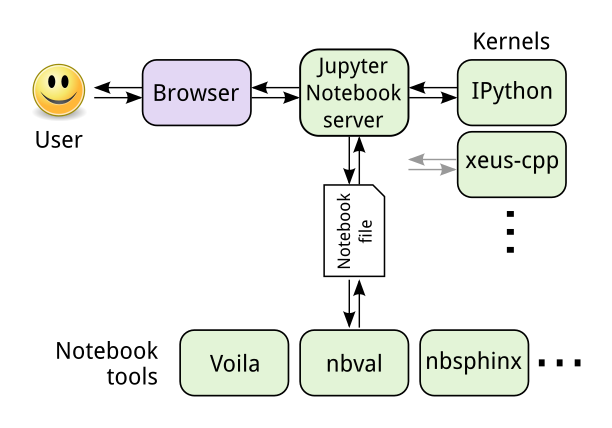
\includegraphics[width=0.6\textwidth]{images/notebook_components.png}
  \caption{The architecture of the Jupyter Notebook, kernels, and tools
        which operate on notebook files}
  \label{fig:notebook-architecture}
\end{figure}


\subsubsection{Methodology}\label{sec:methodology}


\textbf{Proposed improvements of core components of Jupyter (\WPref{core})}\\
We plan to make technical changes to the Jupyter Notebook software to support
real-time collaboration (\taskref{core}{collaboration}),
so that two or more people in different places can work together
on the same notebook. This would significantly enhance the value of
notebooks for collaborative research.
We will also work on making Jupyter software accessible to as broad a
range of users as possible (\taskref{core}{accessibility}).

Further work to bring the code behind JupyterHub and Binder closer together
(\taskref{core}{jh-bh-conv}) will bring a range of benefits, allowing more
flexible sharing of notebooks along with access to remote computing resources
such as those available through EOSC.

Finally, we are explicitly allocating time in \WPref{core} for maintaining
Jupyter software, as well as new development (\taskref{core}{maintenance}).
Maintenance is crucial to creating reliable, sustainable software,
but its cost is often swept under the rug in funding applications
because of the perceived pressure to focus on novelty.

\medskip
\noindent\textbf{Proposed improvements of the Jupyter ecosystem (\WPref{ecosystem})}\\
We further propose improvements of the wider Jupyter ecosystem for
better scientific workflows. In particular, we have identified
possible improvements to:

\begin{itemize}
  \item Binder and its crucial software component \emph{repo2docker}
    (\taskref{ecosystem}{r2d-and-binder}).

  \item Xeus, to better support the C++ programming language in notebooks
    (\taskref{ecosystem}{xeus-cpp}).

  \item Interactive widgets, including tools for 3D visualisation to help
    people make sense of large amounts of data
    (\taskref{ecosystem}{jupyter-widgets}).

  \item Archiving of computational environments to allow reproducible research
    with a focus on the long term (\taskref{ecosystem}{reproducibility}).

  \item Tooling and guidelines
    for using notebooks in education
    (\taskref{ecosystem}{teaching-tools}).

\end{itemize}

We may create new open source software projects in these tasks,
but we will carefully review existing software, both in the
Jupyter ecosystem and beyond, to avoid unnecessary duplication of effort.

\medskip\noindent\textbf{Beyond the improvement of the Jupyter Project
  (\WPref{applications}, \WPref{eosc}, \WPref{education})}\\
Beyond the improvement to the Jupyter core and ecosystem software for EOSC, we plan on
\begin{itemize}
\item Design, implementation, application, demonstration and
  evaluation of new innovative EOSC services
  in multiple demonstrators, that cover research fields such as
  health, astrophysics, photon and neutron science, geosciences and
  mathematics, and also interests of participating SMEs (\WPref{applications}).
\item Operating a \emph{European Binder Service} on the EOSC-Hub and
  enabling provision of Jupyter Services through the EOSC-Hub (\WPref{eosc}).
\item Producing \emph{training and education material} to disseminate
  the ability to do reproducible computational science using the tools
  we develop, among others (\WPref{education}).
\end{itemize}

\medskip
\noindent
\textbf{The science demonstrators}\label{sec:science-demonstrators-in-concept}\\
\emph{Demonstrator: Astronomy (\taskref{applications}{astro})}\label{sec:concept-demonstrator-astronomy}

  The \href{http://cdsweb.u-strasbg.fr/}{Strasbourg Astronomical Data Center} (CDS) is scientific data
  center hosted by the Observatory of Strasbourg. The CDS plays a unique and
  essential role in astronomy by adding value to published and reference data.
  CDS runs astronomical services that
  provide data for the world-wide astronomy research community. Its three main
  services (SIMBAD, VizieR and Aladin) are heavily used with up to one million
  queries per day.  These services be accessed through web interfaces, mainly
  for human interaction, as well as through programmatic interfaces, including
  the standardized protocols defined by the International Virtual Observatory
  Alliance.

\begin{figure}[ht!]\centering
  \includegraphics[width=0.6\textwidth]{python-astro-citations}
  \caption{Mentions of programming languages in refereed Astronomy papers, extracted from ADS. Python usage has increased dramatically in the recent years.}\label{fig:python-astro-citations}
\end{figure}

  Python and notebooks are rapidly increasing in importance for astronomy
  research. Indeed, Python for Astronomy software ecosystem has known a
  constant steady growth in the latest years, as shown in
  figure~\ref{fig:python-astro-citations}. As Python and notebooks integrate
  well together, the Jupyter notebook as an analysis tool is becoming a hot
  topic in the astronomical world: large surveys like the LSST (Large Synoptic
  Survey Telescope) have endorsed the usage of the Jupyter platform for their
    data access portal \cite{lsst2017scienceplatform}.\\


  We will develop a Jupyter-based framework to efficiently access, explore,
  visualize and analyze reference data that are available through CDS services
  as a real example of using open astronomy data.
  We will provide scientific users with a set of customizable Jupyter notebooks
  for visualization and analysis tasks, providing a new level of
  interoperability with python libraries and notebooks as is highly demanded
  by the astronomy research community.

  The focus is on the two following user stories:
    \begin{compactitem}
        \item analysis of catalogue data results, up to billions of rows.
              Tabular data is the typical output of SIMBAD and VizieR data.
        \item modular dashboard-like interface providing a top level
              interactive view of the available data for a given astronomical
              object and enabling loading and analysis of those data.
    \end{compactitem}


\begin{figure}[ht!]\centering
  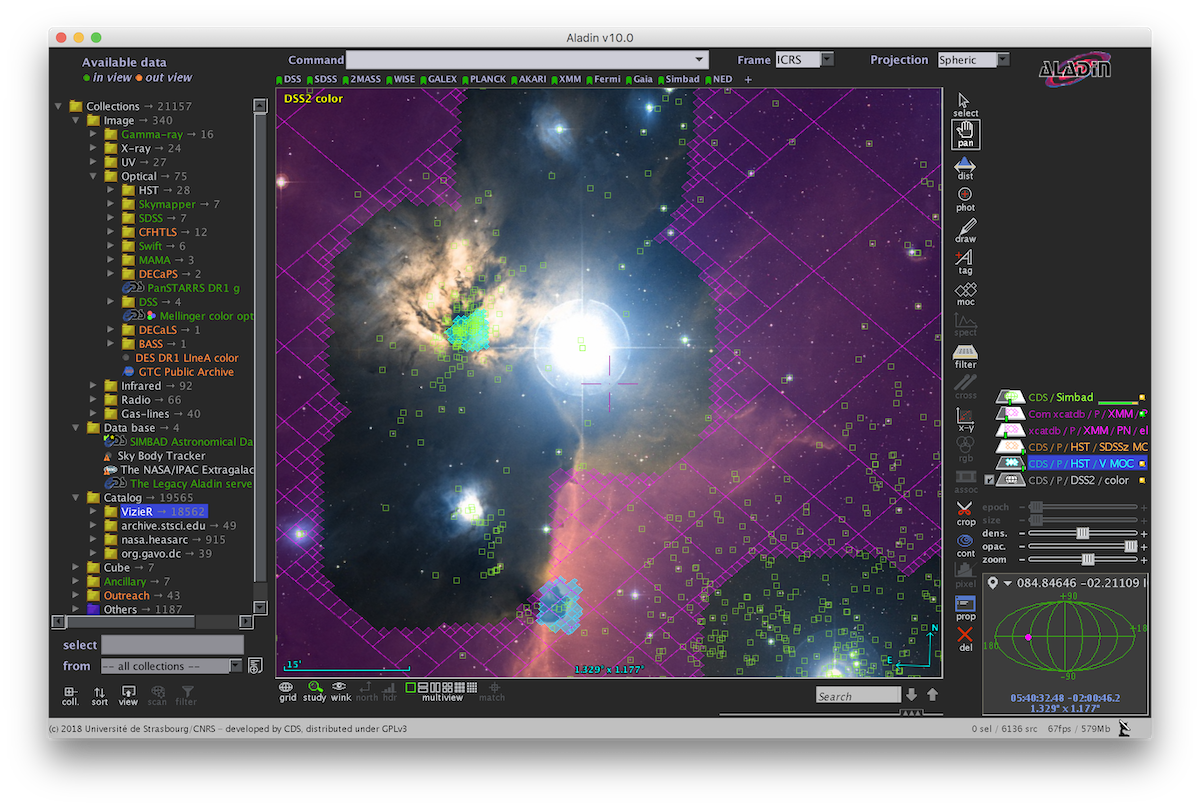
\includegraphics[width=1.0\textwidth]{astro-aladin-snapshot}
  \caption{Simbad objects, XMM and Hubble coverages overlaid on Digital Sky Survey imagery in the vicinity of the Horsehead nebula, and visualized in Aladin Desktop software.}\label{fig:astro-aladin-snapshot}
\end{figure}

  Access to the notebooks will be provided as a one-click action option from
  SIMBAD and VizieR results pages.
  Thus, providing with a one-click way of visualizing, filtering and analyzing
these potentially large tables will bridge the gap between access and analysis
of the data, with zero installation for the user.
  For specific science cases, we will explore rendering of notebooks with
  interactive widgets through Voila \cite{Voila}, as to allow users not familiar with
  Python to benefit from the Jupyter notebook framework.
  Figure~\ref{fig:astro-aladin-snapshot} depicts typical data objects we want to analyse and interact with in the notebooks: images, catalogue data, datasets coverages.

  These new developments will be highly visible to the large number of astronomers who use the CDS services (50,000 unique visitors per month) and such tools are in high demand by these users.

  The CDS expertise in astronomy data and interfaces will be profitably combined with expertise of BOSSEE partners to ensure the deployment of high quality widgets (Simula, WildTree Tech, QuantStack).

\medskip
\noindent\textbf{Demonstrator: Enriched education with Jupyter (\taskref{applications}{teaching})}\label{sec:concept-demonstrator-teaching}

  The Jupyter
  ecosystem offers a versatile environment which has been widely
  adopted in higher education in the recent years. École
  Polytechnique, Université Paris-Sud and other participants from this
  project have been early adopters (see the description of \site{EP}
  and \site{UPSUD}, and also task~\taskref{ecosystem}{teaching-tools}).

  \begin{figure}[ht!]\centering
  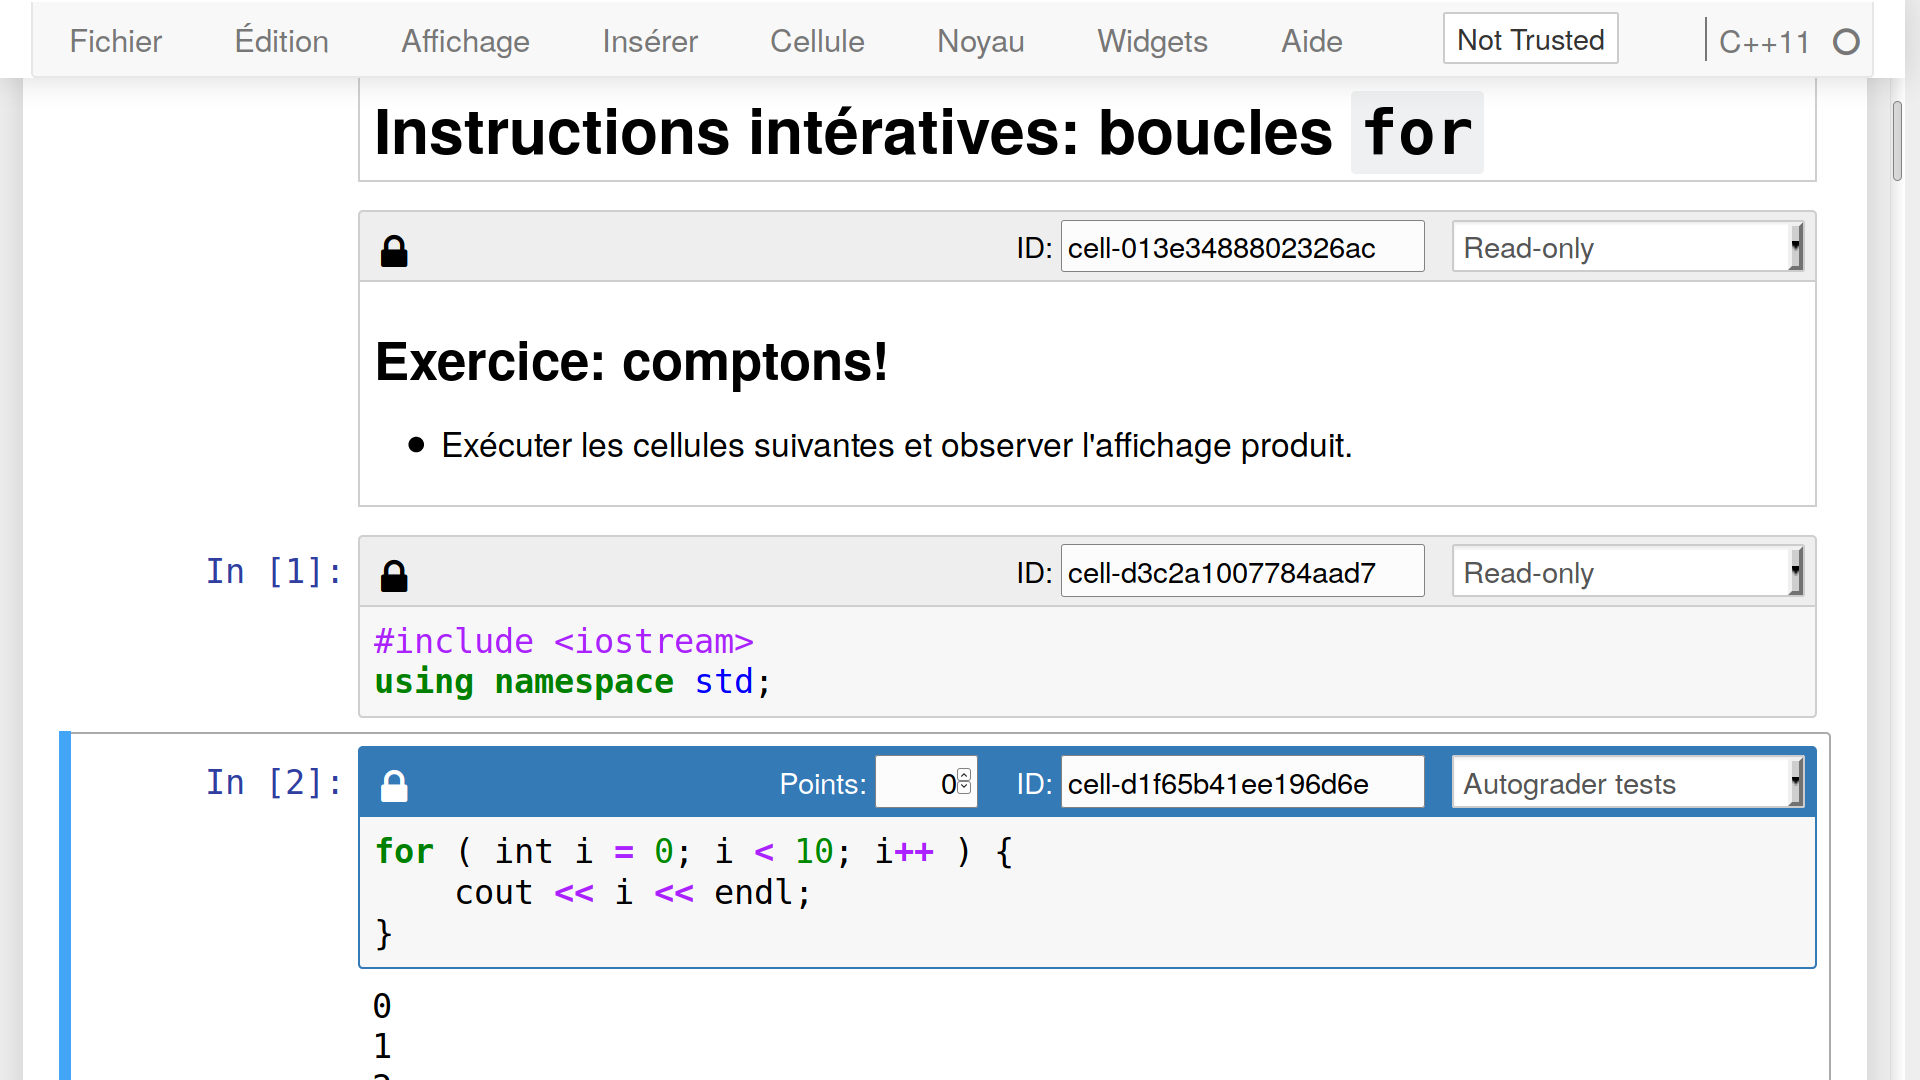
\includegraphics[width=.45\textwidth]{images/teaching-cling}\quad
  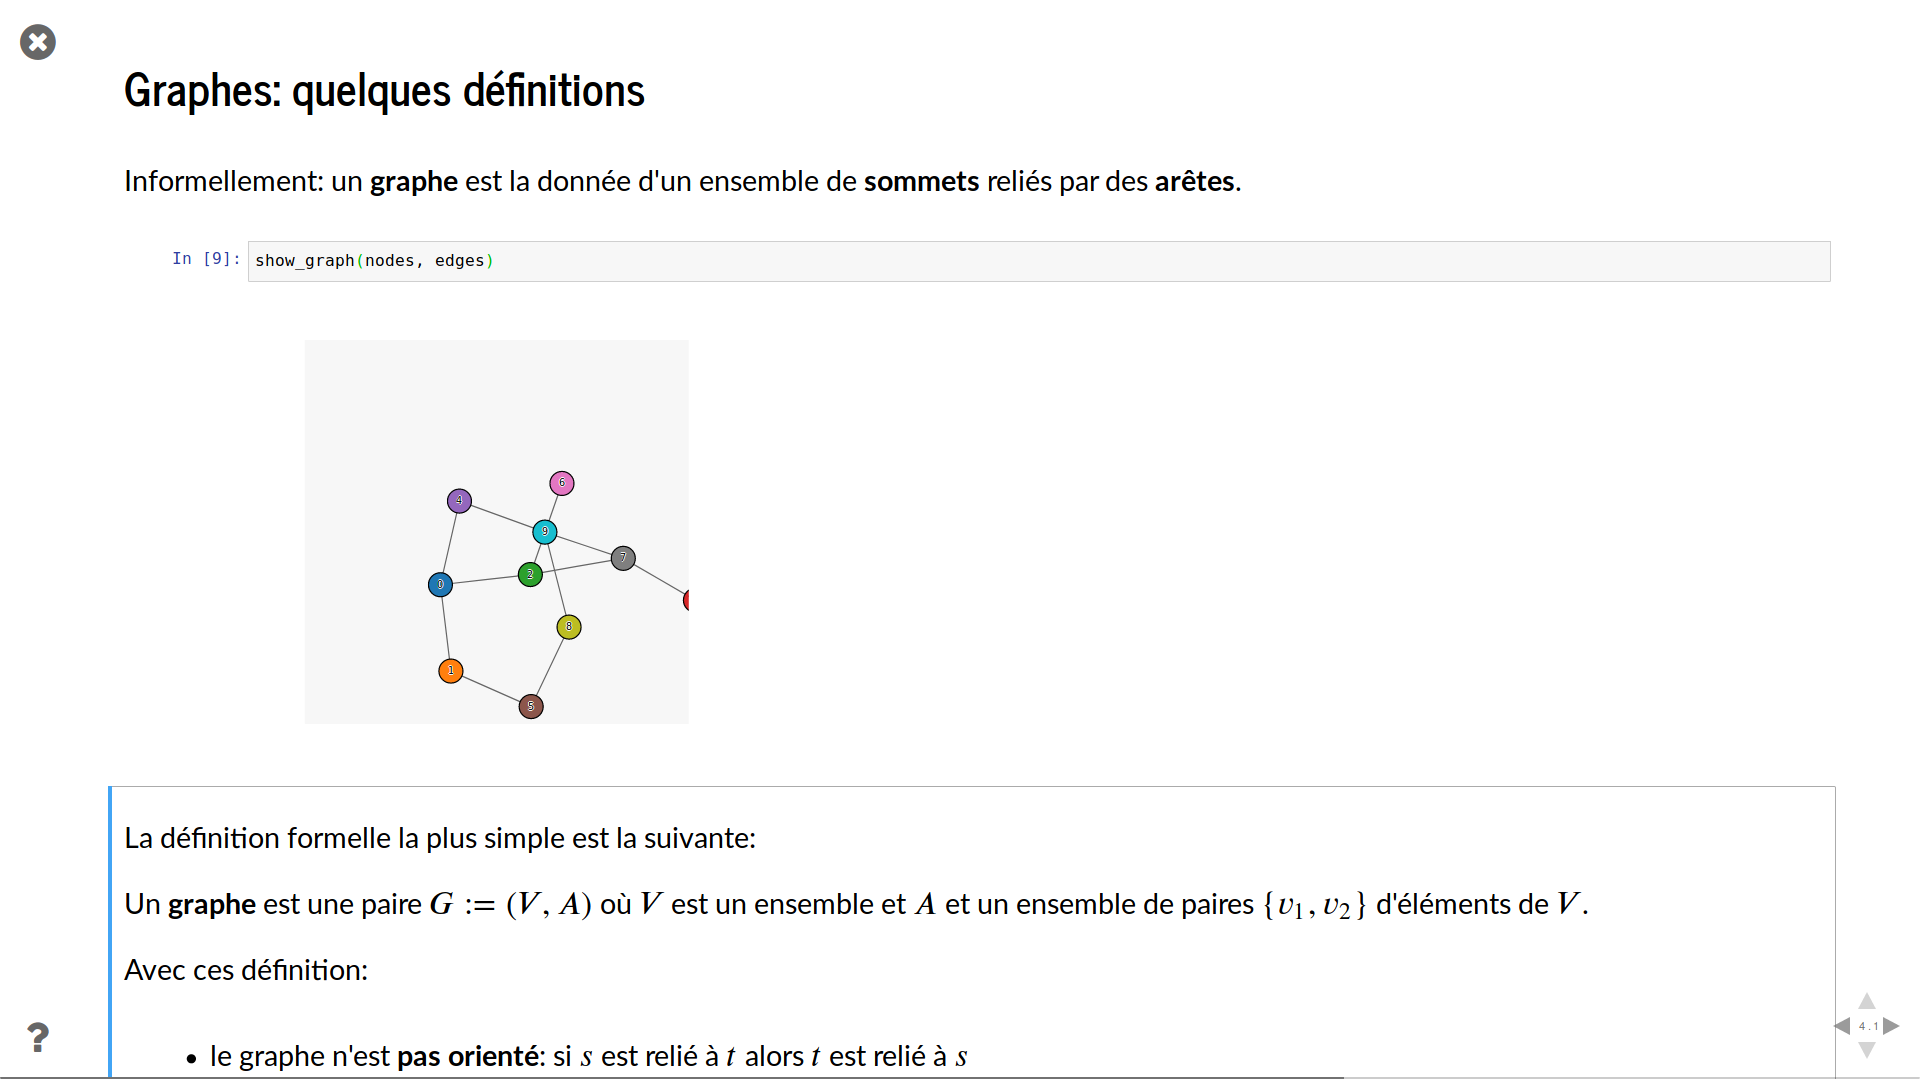
\includegraphics[width=.45\textwidth]{images/teaching-graphs}
  \caption{Jupyter based teaching material from Paris Sud. On the
    left: an exercise sheet for the course \emph{Introduction to
      programming}; this instructor version showcases interactive C++
    execution and automatic grading configuration menus. On the right:
    interactive slides for a graph theory course.}\label{fig:teaching-cling}
  \end{figure}

  We learned the hard way that deploying the Jupyter environment at a
  large scale (e.g. for a university) requires specialized expertise
  (DevOps, software development, ...) which impedes its adoption
  by the greatest number of people. High quality hosted solutions
  (e.g. cocalc, gryd) do exist but are not the final solution when it
  is desired to get higher control on private data, integration with
  the local infrastructure (authentication, shared drive, e-learning
  environment, dedicated hardware, ...), or to use local computing
  resources rather than paid services.

  Further improving the Jupyter environment for education, while
  leveraging it to the greatest number, are therefore key motivations
  for the following tasks of this proposal:
  \begin{itemize}
  \item Tasks~\taskref{core}{jh-bh-conv}
    and~\taskref{eosc}{jh-bh-deployment} will greatly ease the
    deployment of Jupyter environments, with tight integration in the
    existing local infrastructure and full customizability by the
    teachers.
  \item Task~\taskref{ecosystem}{teaching-tools} will improve the
    interoperability with existing e-learning systems, and further
    develop teaching aids for, e.g., material sharing,
    (self)-evaluation, and grade management.
  \item Task~\taskref{applications}{math} will support teaching
    in mathematics through better support for real-time interactivity.
  \item Task~\taskref{ecosystem}{xeus-cpp} will support teaching
    in computer-science and scientific programming through
    better C++ integration in the notebook and will allow to first class students to focus on the
    syntax of the language without distractions such as compiling and
    linking a program.
  \item Task~\taskref{eosc}{eosc} will ease publication and FAIR
    access to course material.
  \end{itemize}

\medskip
\textbf{Demonstrator: Visualisation and control of fluid dynamics in
  Jupyter notebook (\taskref{applications}{application-gpu})}\label{sec:concept-demonstrator-gpu}


In recent years, the lattice Boltzmann method (LBM) emerged as an
interesting alternative to more established methods for fluid flow
simulations. Sailfish-cfd \cite{januszewski2014sailfish} is an open
source implementation of the LBM on General Purpose Graphical Processing
Unit (GPGPU) devices. It is written in Python with real-time
generation of CUDA-C code.  In order to harvest capabilities of GPGPUs
one needs to access the specialized hardware, which usually is
available to researchers as remote HPC resources.  The typical fluid
dynamics research workflow consists of three stages: preparing
boundary conditions, running a simulation, and data analysis. The
first and last stage require capable and responsive user interface for
maniputation and inspection of 3d data.  The Jupyter 3d visualisation
widgets developed in \taskref{ecosystem}{jupyter-widgets} can fulfil
such needs.

Based on previous experience with K3D-jupyter\cite{K3D}
widgets we know that web browser based software can display moderate
dataset during the simulation. As the dataset is becoming larger the
visualisation in the browser turns out to be nontrivial due to
limitations of the browser itself and required large data transfers. It is
an open question how much of data processing should be performed on
server-side and what can be done on the client hardware (i.e. in the
widget in the browser side of the user). Our
experience suggests that there is no clear answer and it depends on
the size of the data and its nature. For example, volume rendering
technique can be very effective on the browser side but infers large data
transfers. One can perform it the server-side, in a distributed way if
the simulation uses many nodes, but the interactivity is limited by
network latency. We will attempt to provide practical
solutions to this issue.
%
  \begin{figure}[ht!]\centering
  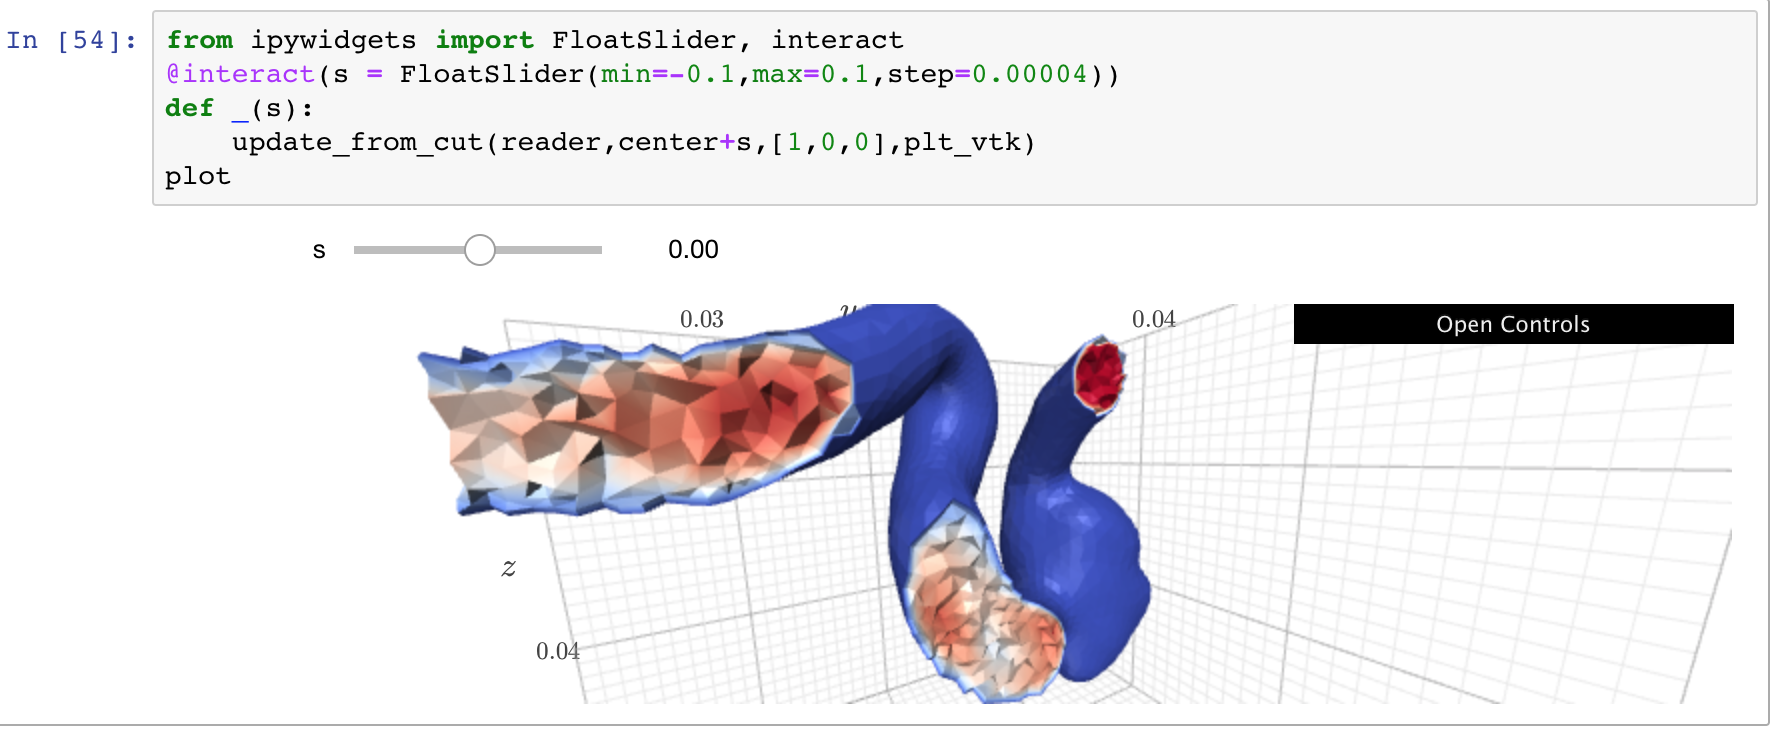
\includegraphics[width=.95\textwidth]{images/k3d_cfd.png}
  \caption{An example showing Jupyter based visualization of velocity magnitude in the blood flow through an aneurysm. It demonstrates use of small interactive widget for selecting cutting plane. Visualization is done by K3D-jupyter widget\cite{K3D}. In this case most of computations are done using VTK library on the server side, K3D-jupyter widget is used to display colored surface mesh. }\label{fig:k3d-cfd}
  \end{figure}


\medskip
\textbf{Demonstrator: Geosciences (\taskref{applications}{geoscience})}\label{sec:concept-demonstrators-geo}

The amount of geospatial data from a variety of sources, including satellite observations, 4D simulations and in-situ observations, contributed by volunteers
or state agencies keeps increasing. In many disciplines, managing this large volume
has become a challenge, and the old approach of downloading datasets for a local
analysis has become intractable.

The heterogeneity of the tools used in different institutions to deal with
large geographical datasets makes it difficult for researchers to share the outcome
of their work in a reproducible fashion.

In this context, Jupyter is now emerging as a standard exploration tool for
geospatial analysis, climate science, geology and by data providers in these areas.

To mention a few,
\begin{itemize}
\item
   the \emph{PanGeo} platform \cite{Pangeo2018} (Funded by the NSF, NASA, and the
   Alfred P. Sloan Foundation) is built upon Jupyter, JupyterHub, Binder, and Dask.
\item
   the \emph{Joint Research Centre Earth Observation Data and Processing Platform}
   (JEODPP) \cite{Soille2018} relies on Jupyter, JupyterHub and ipyleaflet as
   its main user interface.
\item
   the \emph{Google Earth Engine} platform also offers a jupyter-based user
   interface allowing the visual exploration of the data with ipyleaflet
   \cite{GEEJupyterLeaflet2017}.
\end{itemize}

In these three cases, deferred processing is used to restrict computation to
the extent of the area displayed in the map viewer, which allowed these
platforms to scale up to petabytes of data. In all examples, interactive
visualization is a key feature of the platform. Beyond tile-based
2-D visualization, the ability to efficiently process and visualize vector
or 3-D  data is also becoming critical.

The BOSSEE team, which comprises the main authors of the technologies upon
which these platforms are built (Jupyter, JupyterHub, Binder, ipyleaflet),
together with the Department of Geosciences of the University of Oslo, are
in a unique position to bring these technologies together in the context of
EOSC.

This demonstrator will focus on tools for two transversal research projects

\begin{itemize}
\item LATICE (Land-Atmosphere Interactions in Cold Environments)
\url{https://www.mn.uio.no/geo/english/research/groups/latice/}
\item EarthFlows (Interface Dynamics in Geophysical Flows)
\url{https://www.mn.uio.no/geo/english/research/groups/earthflows/}
\end{itemize}

The work items for this demonstrator fall in two main categories:
visualization and geographical data processing tools.

\textbf{Teaching geo-sciences with Jupyter}\TODO{Anne - please see my
  comments in email - this looks odd here (Hans)}

Beyond their use in scientific research, these development will be used in
the class room for teaching master's students with best practices in open
science.

\TODO{The transversal research plays into the desired ``services that
  encourate collaborative interdisciplinary work'' that are desired
  by this call; this is good. Can you imagine that some of these
  facilities can be used via the EOSC? That would be a good
  addition. For example, one could use the BinderHub installation
  that we expect on the EOSC. }

\medskip
\textbf{Demonstrator: Nuclear Medicine application (\taskref{applications}{opendose-analysis})}\label{sec:concept-demonstrators-opendose}

  % Scientific description
  Nuclear Medicine is a field of medicine where radioactive material
  (radiopharmaceutical) is used for diagnostic and therapy. Even though the
  majority of Nuclear Medicine procedures (90\% according to successive EANM
  surveys) are diagnostic examinations, therapeutic applications tend to
  develop and drag more and more attention, for example for the treatment of
  neuroendocrine tumours \cite{Bodei2009}.

  The formalism used to objectively characterise the irradiation process is
  similar for both application types: it was introduced in the late 60s by the
  MIRD (Medical Internal Radiation Dose) committee of the American Society of
  Nuclear Medicine (SNM). This formalism \cite{loevinger1991mird} requires two
  independent quantities; the radioisotope cumulated activity ($Bq.s$) in the
  source (tissue/organ) and the mean absorbed dose to a given target
  (tissue/organ) per radioisotope disintegration (S-value,
  $Gy.Bq^{-1}.s^{-1}$). The S-value calculation requires a clear definition of
  the geometry of the patient (or the model) and radioisotope decay
  characteristics, it can be expressed as a linear combination of
  yields/energies ($J$) and Specific Absorbed Fractions (SAF, $g^{-1}$).

  The calculation of SAFs involves radiation transport modelling and energy
  deposition scoring in anthropomorphic models, usually based on Monte Carlo
  simulation. Historically, SAFs were computed from mathematical models -
  simplistic approximations to human geometry. The advent of voxel-based
  computational models requires a new appraisal of dosimetric data. For
  example, the models recently proposed by the International Commission on
  Radiation Protection (ICRP) include 140 possible radiation sources, leading
  to around 20000 source/target combinations \cite{ICRP2009ICRPPhantoms}. The
  production of SAFs for these models for all possible source regions,
  radiation types and energiesimpul represent an important computation time
  (millions of CPU hours).

  The OpenDose project \cite{Chauvin2017} is a collaborative effort to generate
  reference dosimetric data using various Monte Carlo codes across different
  teams. The collaboration includes at the moment 14 research teams over 18
  institutes.  The idea is to trigger the collaborative development of a
  reference database, freely available, proposing dosimetric data applicable in
  a context of nuclear medicine dosimetry (for therapy and diagnostic
  applications). A major aspect of the project is the development of tools
  ensuring traceability and reproducibility of generated results.

  % Technical description
  OpenDose data is produced using the five most represented Monte Carlo
  simulation software in medical applications: Geant4/GATE, MCNP, EGS, PENELOPE
  and Fluka. Each simulation consists of calculating radiation transport in
  anthropomorphic models for specific parameters (source organ, particle type,
  energy, model and number of primaries to simulate). Every simulation produces
  binary (3D matrices) and ASCII files for a total of $\sim$150MB / simulation.
  The 3D matrices contain energy deposited per voxels, and ASCII files contain
  pre-processed data corresponding to energy deposited per regions such as
  organs and tissues. These raw outputs are later processed into dosimetric
  data such as Specific Absorbed Fractions (SAFs) and S-values.

  Producing data for one model (ex. adult female) requires $\sim$30,000
  simulations, with the workload shared between the different teams and
  software.

  The data produced by all the teams is currently centralised at the Cancer
  Research Center of Toulouse (CRCT), processed and fed into a local SQL
  database at CRCT.

  This collaborative effort raises some challenges:
  \begin{compactitem}
  \item Data production: a total of 750,000 hours of CPU time is needed per
    model.
  \item Volume of data: one model represents TB of raw data that can be
    heterogeneous from the different teams.
  \item Data analysis: raw data has to be processed into dosimetric data in a
    robust and reproducible way.
  \item Database: has to be efficient and handle all the data (raw and
    processed).
  \item Visualization: display and compare results from all teams.
  \end{compactitem}

Figure
  \ref{fig:opendose_framework} shows the overall framework of the project and
  how data will be managed.

  \begin{figure}[t!]
    \centering
    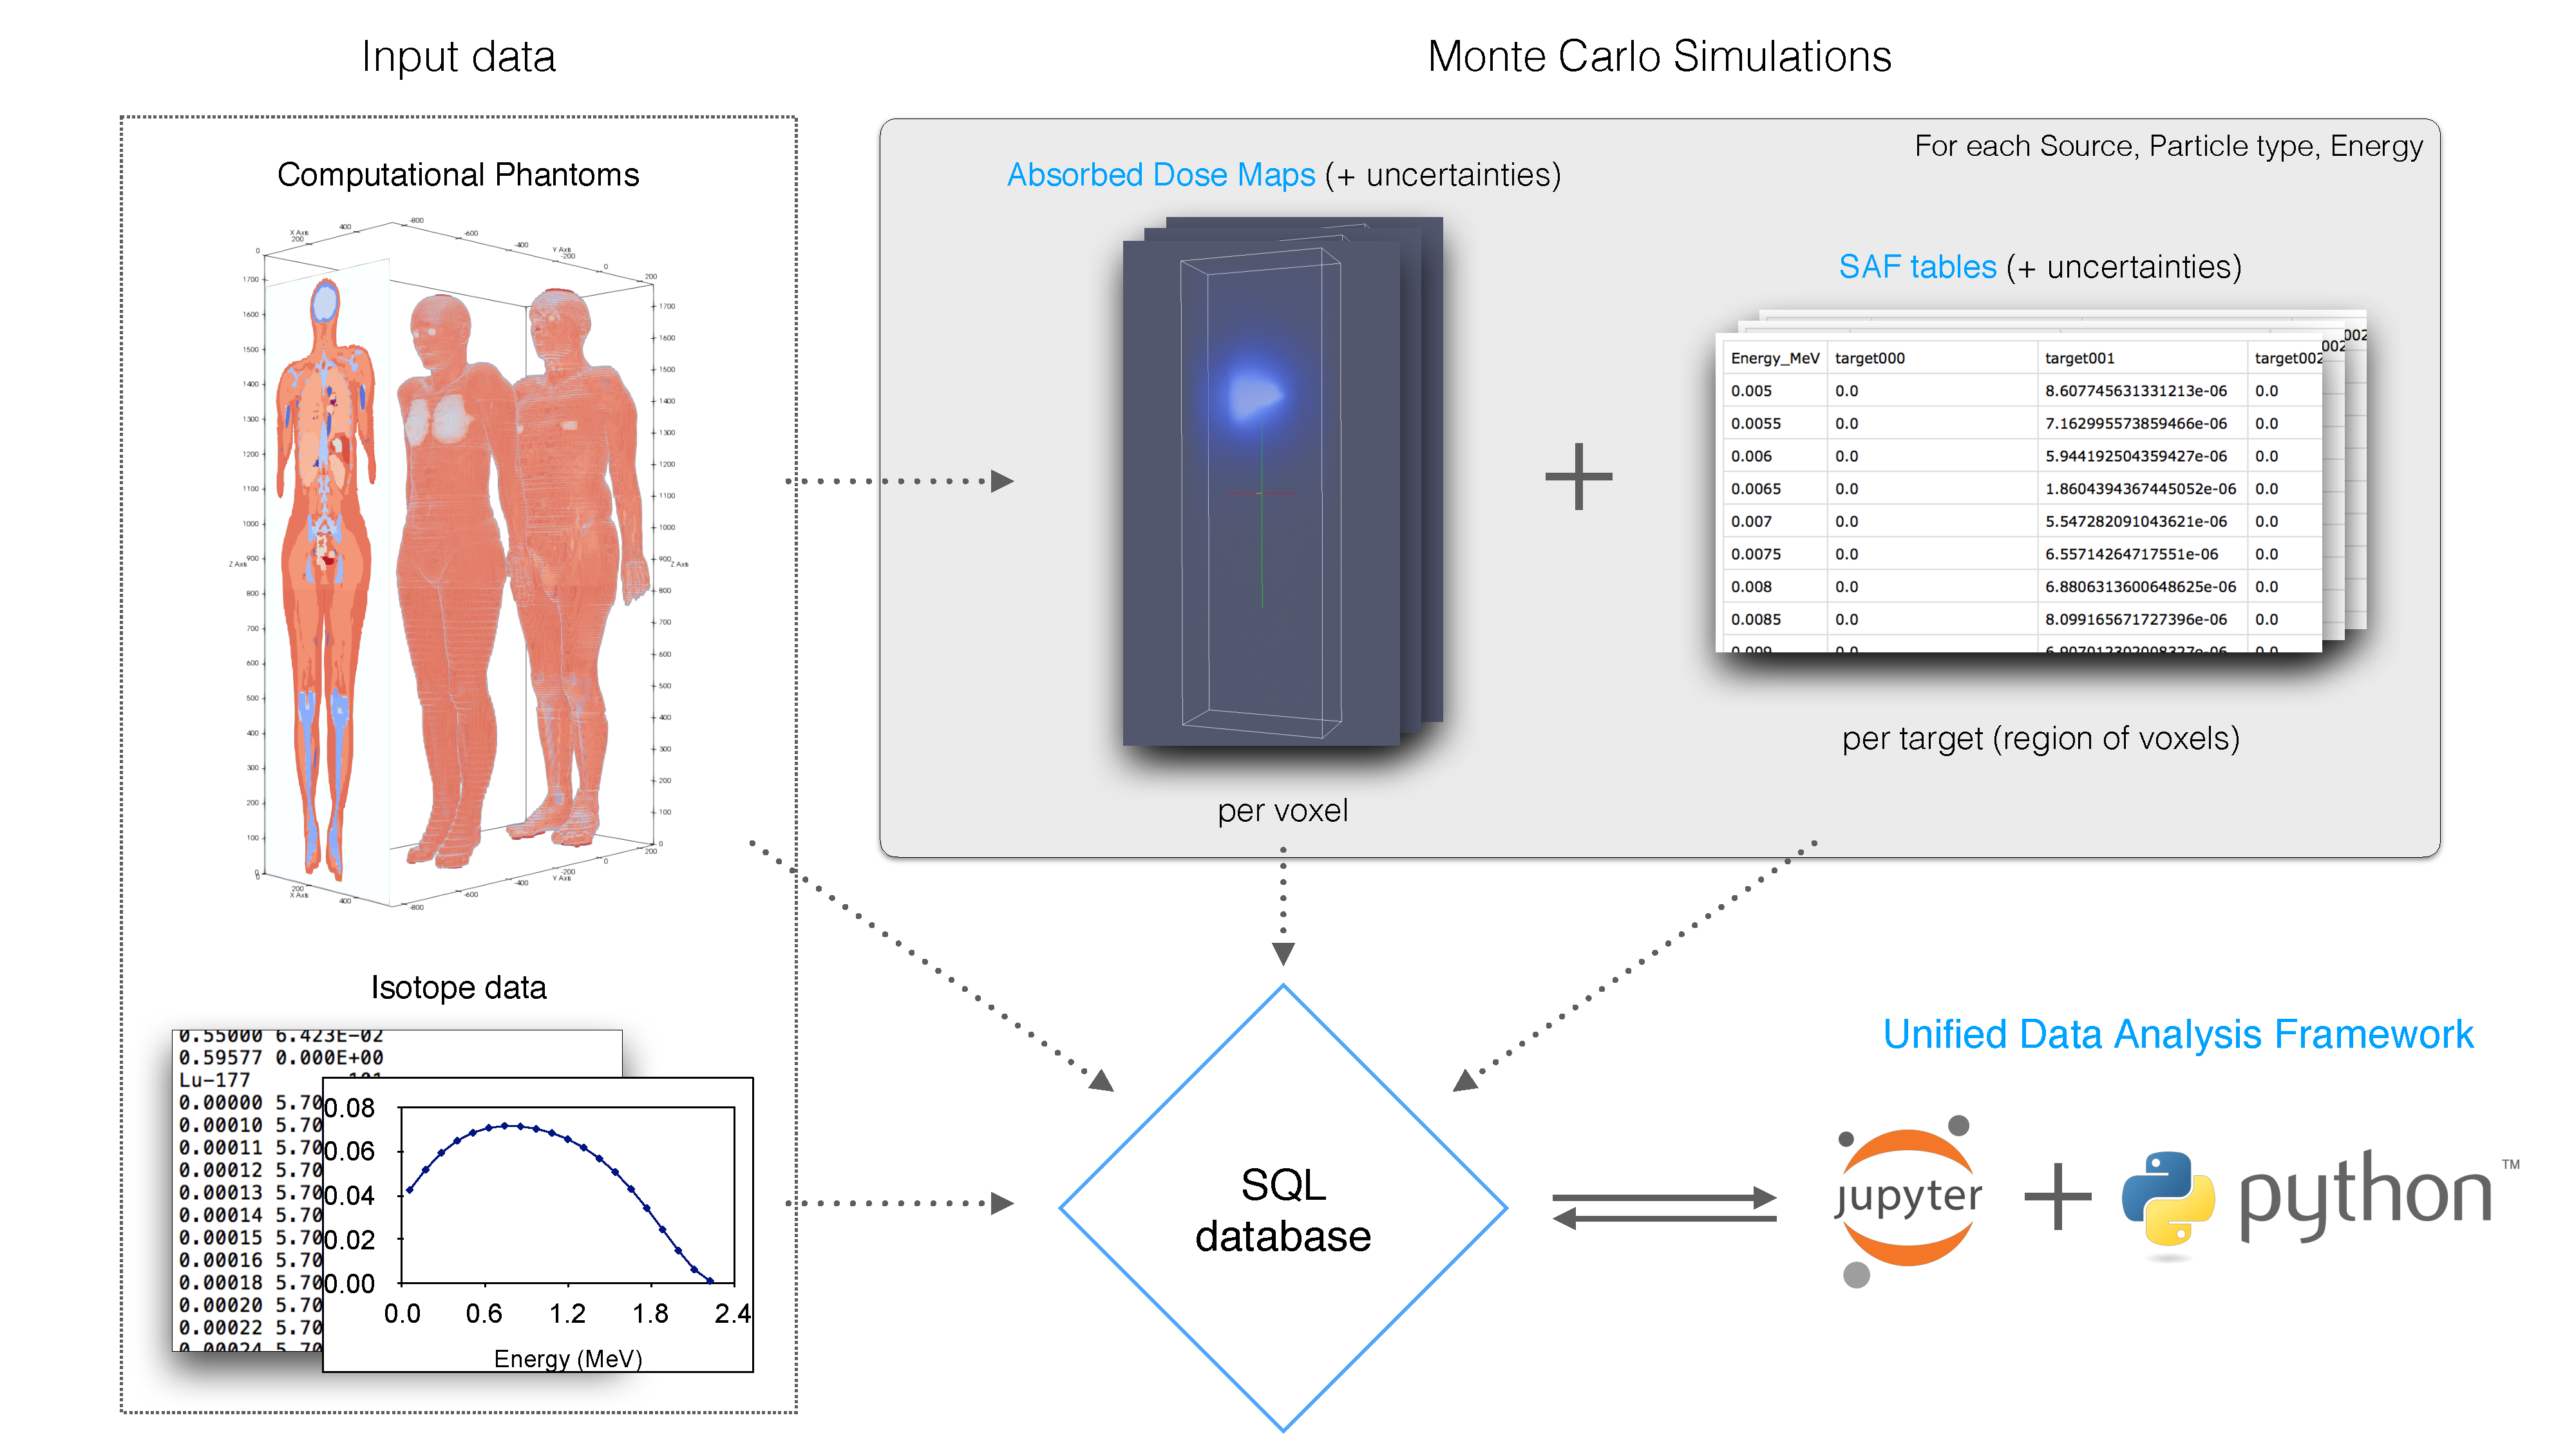
\includegraphics[width=1.0\textwidth]{images/opendose_framework.pdf}
    \caption{OpenDose project overall framework including the unified data
    analysis to be developed in this task.}
    \label{fig:opendose_framework}
  \end{figure}

  By building a set of tools to access and process data, this will ensure the
  production of traceable and reproducible dosimetric data for the OpenDose
  project members.

  Another major aspect of the OpenDose collaboration is to provide an open
  access to the generated dosimetric data. For that purpose a website is under
  development to allow data download and simple dosimetry calculations. For
  users who need more advanced calculations, a dedicated Jupyter workspace will
  provide a set of tools to easily access, process and display the OpenDose
  data.

\medskip
\textbf{Demonstrator: Interactive Mathematics with Jupyter Widgets (\taskref{applications}{math})}\label{sec:concept-demonstrator-math}

  \TODO{Ideas to reinforce the ties with EOSC services welcome!}

  Computations have played a long time and ever increasing role for
  research and teaching in (pure) mathematics, to explore, search and
  check for conjectures, or better understand algorithmic ideas. This
  led to the development of a whole ecosystem of mathematical
  software, many of which are open source. Given the huge variety of
  mathematical objects and workflows, the Read-Eval-Print-Loop (REPL)
  paradigm -- on which Jupyter is based -- is particularly suitable:
  the user interacts with the system by typing commands that use its
  library of mathematical features, often combined with personal code.
  In fact, the REPL and notebook paradigms of Jupyter as well as some
  of its interactive features were largely inspired by that of
  computer algebra systems such as Maple, Mathematica, or SageMath.

  One major action of the OpenDreamKit project was to foster the
  convergence between the Jupyter and math software ecosystems:
  nowadays Jupyter can be used as a uniform user interface for most
  major systems: e.g. GAP, OSCAR, Pari/GP, SageMath, Singular, and
  even for C++ libraries. This interface is being widely adopted: for
  example, Jupyter has become the standard user interface for
  SageMath, enabling to phase out its former bespoke notebook; by now,
  thousands of jupyter notebooks for SageMath are publicly shared
  (6000+ on GitHub alone).

  Thanks to this prior art, the mathematical community will
  immediately enjoy all the benefits brought by EOSC-based generic
  Jupyter services, including eased collaboration, sharing, archival,
  and reproducibility.

  The next step to maximize attractivity and impact in the
  mathematical community, and this is the aim of this task, is to go
  beyond the REPL paradigm, and \textbf{leverage the real time
    interactivity and flexibility brought by Jupyter widgets for
    Mathematical purposes}. Think making it easy for a teacher or
  researcher to build and disseminate via the EOSC a mini applications
  or dashboard enabling the graphical exploration of a whole range of
  mathematical inputs, with real-time visualization of the associated
  outputs.

  The unique challenge comes from the huge variety of mathematical
  objects that the user may want to visualize and interact with, and
  the variety of graphical representations. Co-design is central here,
  as building a bespoke interactive visualization entails a
  combination of technology skills (e.g. javascript development) and
  business knowledge (designing the interaction and visualization).
  The role of Research Software Engineers is to leverage the
  technology by encapsulating the technical difficulties into flexible
  and easy to use tool boxes from which mathematicians can build
  mini-applications tailored to their needs.

  Within OpenDreamKit, we conducted experiments to explore this
  venue~\cite{ODK_D4.16}. One specific focus was to enable not only
  \emph{interactive visualization}, but also \emph{interactive
    editing}: being able to graphically modify the mathematical object
  being visualized; this enable the interactive exploration of how the
  modifications affect its properties, or to use the editor as input
  widget for a larger applications or dashboards. The outcome of this
  task are the development of two prototypes in SageMath
  (\software{sage-combinat-widget}, a library of widgets for
  combinatorics, and \software{sage-explorer} a generic dashboard for
  interactive browsing and introspection of mathematical objects), and
  contributions to \software{Francy}, an Interactive Discrete Math
  Framework for \software{GAP} and \software{SageMath}.

\medskip
\textbf{Demonstrator: Reproducible photon science workflows at
  European XFEL (\taskref{applications}{reproducibility-xfel})}\label{sec:concept-demonstrator-photonscience}


  European XFEL is a research facility that provides X-ray Free
  Electron Laser (XFEL) light to image structures at the nanoscale. It
  is currently the world's most brilliant laser, created in a 3.4km
  long tunnel, and supporting user experiments since September
  2017. These imaging capabilities from European XFEL and similar
  services from synchrotron and neutron sources, underpin lots of
  fundamental and applied research, in domains ranging from fundamental
  physics and material science to biochemistry and drug design. Some
  example data is shown in figure \ref{fig:photon-science-example}.

  All of the data recorded at European XFEL will be made freely
  available after an embargo period of three years
  \cite{EuXFEL-datapolicy-2017}. This provides scientific transparency
  and is expected to enable better exploitation of the data, as more
  researchers than those conducting the experiments have access to the
  results. If the analysis steps are not carefully recorded, there is a risk
  that the necessary understanding of the data is lost by the time it
  is made public or subsequently, greatly reducing its scientific
  value.

  We are keen to complement this open data access to the actual data
  with open access to reproducible data analysis, to confirm
  conclusions drawn and to significantly lower the barriers for
  re-analysis with new tools or for new research purposes.

  A task in the EC funded project Photon and Neutron Open Science
  Cloud (PaNOSC) is using the Jupyter Ecosystem tools as they are in
  2019 to provide interactive data analysis services to complement the
  data: through use of Jupyter Notebook and exploitation of the
  mybinder.org service, this activity will reduce the barrier for
  interactively exploring the data, understanding and making use of
  the data, and to do this through a central portal such as EOSC.

  Here, we combine and use the new developments of this
  proposal to enable new qualities of open science services, and to
  demonstrate the potential impact of these improvements for a wide
  set of EOSC services through a demonstrator in Photon Science.

  \medskip

\begin{figure}[tb]
    \centering
    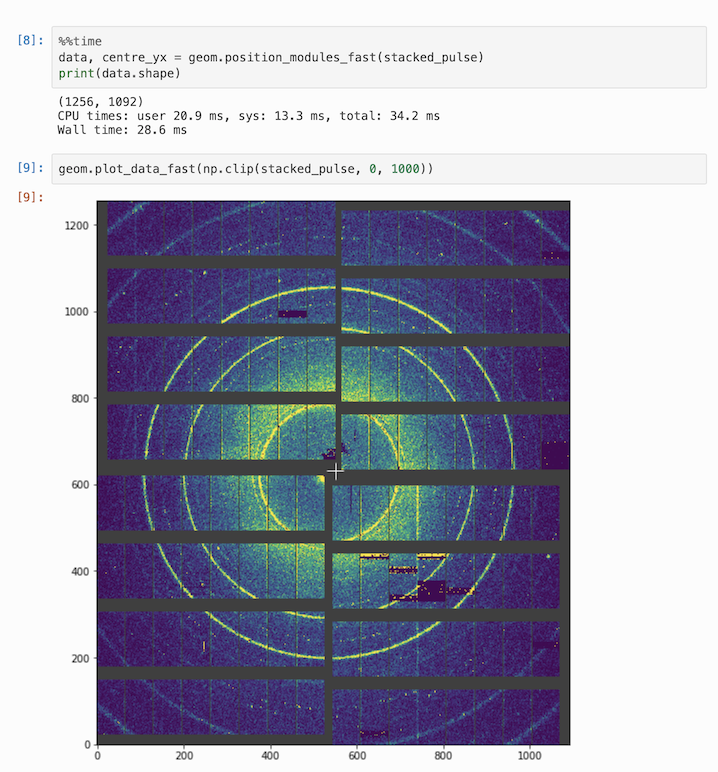
\includegraphics[height=0.27\textheight]{images/photon-science-prototype1.png}
    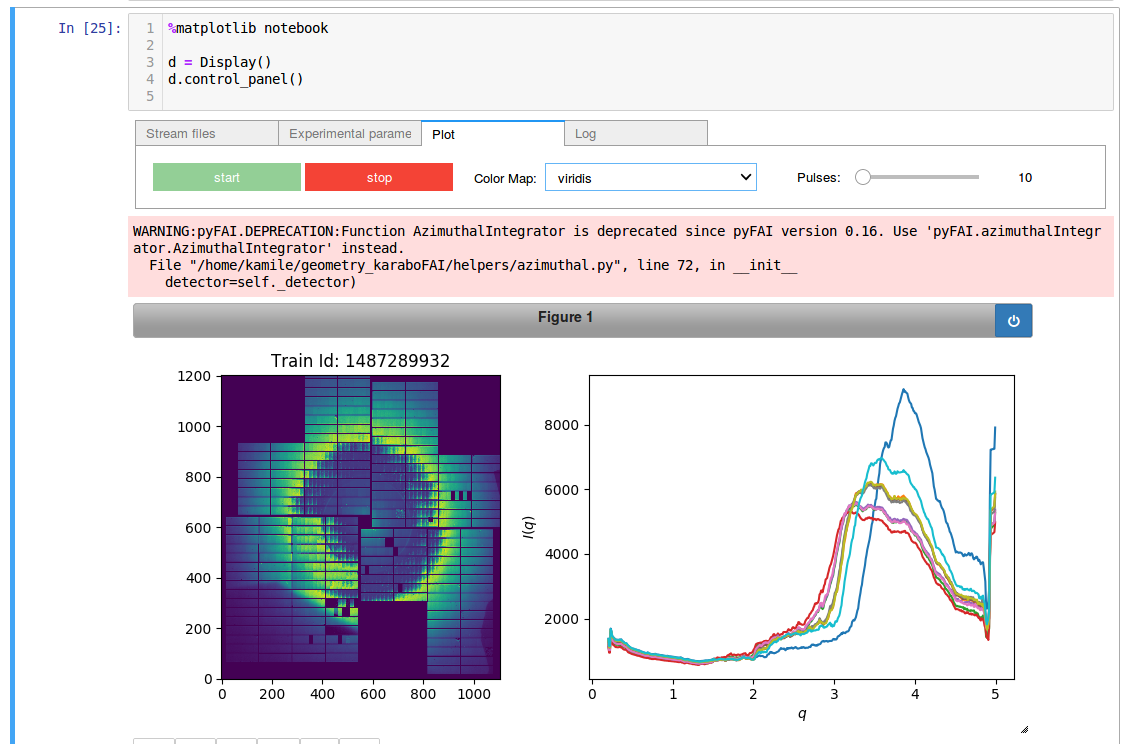
\includegraphics[height=0.27\textheight]{images/photon-science-prototype2.png}
    \caption{Prototypes for data analysis of 2d x-ray detector images
      in the Jupyter notebook, relating to the
      photon science use case.
      % task reference in caption doesn't work
      % \taskref{applications}{reproducibility-xfel}.
      \emph{(Left)} Data from crystallography
      scattering experiment. \emph{(Right)} Azimuthal integration of detector
      data as one step in the data analysis workflow.}
    \label{fig:photon-science-example}
  \end{figure}


  \textbf{Context}

  The very first experiments at European XFEL
  produced as little as 45 terabytes of data on average, but as the
  facility develops, the amount of data produced per time is expected
  to grow substantially: Given the rate of light pulses, there is the
  potential to produce up to a petabyte of data within the beam time
  of one experiment (typically one week). These significant amounts of
  data need to be complemented by complicated workflows to convert the
  data into insight through data analysis. Derived results of such
  data analysis are typically much smaller in size and useful to
  archive together with the raw data. To explain how they have been
  obtained, the particular workflow of data analysis also needs to be
  archived.

  \medskip
  \textbf{Vision}

  At European XFEL we will use Jupyter notebooks to facilitate
  this workflow: the simplest model would be to use one notebook per
  workflow. Once the data capture from the experiment is completed,
  this notebook can be executed (without being displayed in a web
  browser) to start processing the data. When the notebook has
  completed execution, it is saved, and contains the analysis results
  (it may of course also created files on disk as part of the
  process).

  A particularly useful aspect of the notebooks is that they mix data
  analysis commands with outputs, and that the notebook provides a
  complete (and thus reproducible) summary of the data analysis when
  it succeeds with the execution. Should the execution fail, for
  example half-way through the notebook, then derived results obtained
  prior to the error occurring are preserved and can be inspected. The
  error is embedded in the notebook and appears after the command that
  has triggered the error; which helps with debugging the process.

  This is of particular interest as the data analysis processes at
  European XFEL may fail not because of software errors but due to
  variation in the data that require (manual) expert adjustments of
  parameters. The ``failure'' of such an analysis workflow
  (represented through the Notebook) is thus not exceptional, but a
  common occurrence. The scientist conducting the experiment is
  sufficiently skilled to modify the parameters and wants to either
  re-execute the notebook from the beginning or to continue from the
  point of failure. The notebook caters for both use cases. The
  modified notebook would need to be preserved of course to provide
  reproducibility of the derived results that the notebook has
  computed.

  We are aiming for re-executability of the notebook for the lifetime
  of the data. The life time of the archived data at European XFEL is
  currently guaranteed for 5 years and aimed to be 10 years
  \cite{EuXFEL-datapolicy-2017}. It is possible though, that data used
  for publications will be preserved for longer, and it would be
  highly desirable to keep the data analysis re-executable for the
  same period of time, potentially well exceeding 10 years.


\draftpage
% ---------------------------------------------------------------------------
%  Section 1.4: Ambition
% ---------------------------------------------------------------------------
\clearpage
\TOWRITE{ALL}{Proofread 1.4 Ambition pass 2}

\subsection{Ambition}

\eucommentary{1-2 pages}

\eucommentary{-- Describe the advance your proposal would provide
  beyond the state-of-the-art, and the extent the proposed work is
  ambitious. Your answer could refer to the ground-breaking nature of
  the objectives, concepts
  involved, issues and problems to be addressed, and approaches and methods to be used.\\
  -- Describe the innovation potential which the proposal
  represents. Where relevant, refer to products and services already
  available, e.g. in existing e-Infrastructures.}

BOSSEE's ambition is to \textbf{improve the global accessibility} of scientific
tools, results, ideas, data and data analysis;
\textbf{enabling collaboration} among researchers and between researchers and the public.

The world's computational resources are
constantly growing and science is producing ever-more useful and
interesting data.  But \textbf{how do we enable the European and global
communities to make use of that data?}  And \textbf{not just researchers}, but
the public as well?  Open science is a principle of making research
results as broadly accessible and useful as possible.  The first,
minimal step for this is making publications free to access.  The
second step for computational research is to make code and data
publicly accessible, enabling transparency and facilitating
reproducibility and verifiability of results.  But \textbf{merely making these
resources technically available is not the best we can do}.  There can
be many challenges with software, such as environment specifications
and resource requirements, that can be an impediment to the transition
from `technically available' to `practically useful.'  With the tools
of the open source open science community and the resources of the
European Open Science Cloud, we can do better.

The Jupyter ecosystem consists of a \textbf{large, global community} of
developers and researchers producing software focused on interactive
computation and communication, and is \textbf{widely used by millions} of
individuals in numerous scientific fields, ranging from molecular
biology \cite{Wang2016} to materials science \cite{Hughes2014},
astronomy \cite{Baron2017} and climate science
\cite{Laken2015,Laken2015b}.  Jupyter software is permissively
licensed under the Berkeley Software Distribution (BSD) license,
allowing anyone to use Jupyter software for free, and even build
derivative commercial products, as has been done in the cases of
Google Colaboratory, Microsoft Azure Notebooks, IBM Watson Studio, and
others.  By contributing to the Jupyter ecosystem,
\TheProject maximises its impact, immediately benefiting the existing
large Jupyter community, and increasing the likelihood that
\TheProject's results will be maintained by the community after the
end of formal funding.

When it comes to Jupyter and Open Science for EOSC, we aim to improve the
\textit{status quo} by bringing the two together:

\begin{itemize}
\item Improve software in the Jupyter ecosystem to \textbf{better serve Open
  Science}.
\item Enable researchers and the public to \textbf{better perform and benefit
  from Open Science}, through software, services, and education.
\end{itemize}

Open Science that truly benefits society must be more than merely
technically accessible.  Individuals must be able to find the
resources they want and interact with them.  Ideally, they should be
able to ask new questions of models and data published by those that
came before.  This is where \TheProject fits in.  Excellent research
is being performed in all scientific fields, but making those results
practically accessible and engaging to others is a challenge.
Jupyter notebooks enable publishing code and data in a form that is
interactive, where readers can see code, run it, and see results.
They can then modify the code and produce new data and charts that the
first authors may not have considered.  Jupyter does not solve the
software installation problem, however, which can be significant for
scientific software.  For a publication to be truly interactive or
reproducible, it must include a computational environment (or a
sufficiently precise description of one such that it can be recreated)
in order to reliably be able to run for another individual.  Services
and tools such as Binder and repo2docker have started to demonstrate
that this can be facilitated: by
publishing a description of the requirements to run the software,
repo2docker is able to recreate a computational environment with
everything needed to run the software, including a Jupyter
environment for interactively exploring the resource.  Binder wraps
this in a web service, enabling immediate, free sharing of
computational results on the web, with no requirements of readers
other than a web browser.  By developing these tools further, and deploying Binder or similar services on
EOSC infrastructure, EOSC enables researchers to
(i)~\textbf{make their results available} through EOSC,
(ii)~allows other researchers to \textbf{extend that research within minutes} or hours,
and (iii)~\textbf{enables the public to interact with the
science they are funding}.

By cooperating with specific applications from diverse domains in science and education,
we ensure and demonstrate that the work is valuable to a broad community of researchers, students, educators, and the public.
All together, Jupyter and Binder enable the migration of the open
science community from static publication to \textbf{truly interactive,
reproducible publications}.


%%% Local Variables:
%%% mode: latex
%%% TeX-master: "proposal"
%%% End:

%  LocalWords:  eucommentary textsuperscript textregistered textsuperscript specialised
%  LocalWords:  textregistered recomputation textbf textbf rigourous centred flagshsip
%  LocalWords:  subsubsection realisation textit


\draftpage
% ---------------------------------------------------------------------------
%  Section 2: Impact
%  ---------------------------------------------------------------------------
\clearpage
% ---------------------------------------------------------------------------
%  Section 2: Impact
% ---------------------------------------------------------------------------


\section{Impact}
\label{sec:impact}

The central impact of the \TheProject project will be a significant improvement
and extension of the Jupyter tools and ecosystem described in section \ref{sec:project-jupyter}
to facilitate open science and reproducible research,
and their wide availability on the European Open Science Cloud.
While this will initially be developed alongside applications for our
own institutions, we expect the tools we develop to be useful to a much larger
group of researchers, as data analysis and simulation are now crucial parts
of most academic disciplines.

Jupyter-based technology will be especially valuable given the decentralised
nature of EOSC. Large-scale experiments often produce so much data that it is
impractical to transfer the data to another site for analysis.
At European XFEL, for instance, hundreds of terabytes of data may be recorded
for a single user experiment. The analysis steps thus need to run where the
data is stored, even if the scientist has returned to their home institution
far away. As the Jupyter Notebook interface runs in a web browser,
it is readily usable for remote access.

In addition, \TheProject will produce highly visible demonstrations of
notebooks for open science in targeted scientific disciplines.
The result will be innovative new prototype services that will provide
direct benefits to the early adopters in various research fields.
Moreover it will serve as a demonstration of a strategy for open science
using notebooks that will be applicable across many domains.

EGI supports the e-Infrastructure uptake of several ESFRIs in the EOSC-hub project.
Several of these already experiment with Jupyter (either using the EGI's JupyterHub
service, or community specific installations). These communities will
be reached out to by
EGI directly in the EOSC-hub project, and through the annual events organized by EGI
around EOSC: EOSC-hub weeks, the DI4R conferences and EGI conferences. During these
events EGI will contribute to promote the adoption of the project results.

\subsection{Expected Impacts}

\eucommentary{Please be specific, and provide only information that applies
to the proposal and its objectives. Wherever possible, use quantified
indicators and targets.\\
Describe how your project will contribute to:\\
-- the expected impacts set out in the work programme, under the relevant topic
(including key performance indicators/metrics for monitoring results and impacts);\\
-- improving innovation capacity and the integration of new knowledge
(strengthening the competitiveness and growth of companies by developing
innovations meeting the needs of European and global markets; and, where
relevant, by delivering such innovations to the markets;\\
-- any other environmental and socially important impacts (if not already
covered above).\\
Describe any barriers/obstacles, and any framework conditions (such as
regulation and standards), that may determine whether and to what extent
the expected impacts will be achieved. (This should not include any risk
factors concerning implementation, as covered in section 3.2.)}

The expected impact of \TheProject with respect to the
work program is detailed in the table below.

\begin{center}
\begin{tabular}{|m{.3\textwidth}|m{.7\textwidth}|}\hline
  Expected impact & \\\hline


  Integrating co-design into research and
  development of new services to better support scientific, industrial and
  societal applications benefiting from a strong user orientation &
  The Jupyter tools have always been driven by a close connection to users; since
  the project began as IPython in 2001, many of the developers have been
  scientific researchers using the tools as they developed them. More recently,
  when Jupyter has benefited from dedicated developer time, developers have
  remained in academic institutions, in the kind of role now referred to as
  'research software engineers', allowing day-to-day interactions with
  researchers using Jupyter in a wide range of fields.

  By supporting developers in various research institutions where the improvements
  will be used as they are developed, \TheProject will continue this invaluable
  collaboration.

  The improvements and extensions of the core parts of the Jupyter system are
  being co-designed by technical, industrial and scientific experts in the
  BOSSEE project, so that they will be widely applicable in new innovative
  services across most academic disciplines.
  The impact of this approach for enabling scientific use of notebooks is expected
  to be very high because it is a direct response to the strong demand from
  scientists for improving the productivity and reproducibility of their work.
  The notebook approach is being embraced in many scientific disciplines, so the
  proposed services to be developed in BOSSEE are strongly oriented to the user needs.

  \\\hline

  Supporting the objectives of Open Science by
  improving access to content and resources, and facilitating interdisciplinary
  collaborations &
  Jupyter notebooks have seen rapid uptake in many kinds of research,
  because they bring together the essential elements of the modern scientific
  computational workflow (from data collection to publication and open sharing)
  in the familiar format of a scientific notebook, with powerful functionality
  for access to scientific content for analysis and visualisation.
  Notebooks also embody the core concepts of open science by providing a
  mechanism to reproduce results in publications, and collaborative
  sharing of not just scientific results, but of the code that produced them.

  We expect the use of notebooks in EOSC to improve access to scientific code:
  digital documents and notebooks encourage publishing workflows, whereas code in
  scripts or manual interactive workflows are often kept by the researchers who
  performed them. The focus on clarity and reproducibility also helps to ensure
  that data is meaningfully accessible, by preserving essential understanding to
  make sense of the raw data.

  We have already seen a good example of the Jupyter ecosystem facilitating an
  interdisciplinary collaboration: the LIGO scientific collaboration shared
  notebooks detailing the data processing steps which led to the discovery of
  gravitational waves, using the Binder service to allow anyone to re-compute
  the published plots. Scientists with no background in gravitational waves
  studied these notebooks and improved the signal processing.
  In this proposal, we want to provide this ability to a wider audience through
  EOSC, including for disciplines which rely on processing much larger volumes of
  data \cite{ligo-open-science}.

  The astronomy application in \TheProject (\taskref{applications}{astro})
  is designed to provide a new level of interoperability of
  reference astronomy data within Jupyter notebooks.
  By connecting new notebook capabilities to existing and highly used services,
  we expect to have impacts for the users and also for the service provider.
  The scientific users will have access to new capabilities,
  and we anticipate adoption of new innovative ways of using the data.
  We also expect an impact on the services themselves, in terms of usage,
  but also in terms of capturing precious information and feedback on
  how to evolve these services to best support open and collaborative use of
  the data and services.

  \TOWRITE{ALL}{More impacts for other applications/demonstrators ...}
  \\\hline

  Fostering the innovation potential by opening up
  the EOSC ecosystem of e-infrastructure service providers to new innovative
  actors &
  Jupyter is a collection of open source software built around openly documented
  protocols and formats, along with familiar technologies such as HTML and the
  Python programming language. It's easy for third parties to create new
  tools and services using and integrating Jupyter, as evidenced by the thriving
  ecosystem of tools already in development, both by commercial and non-commercial
  actors. To highlight just one example, the first version of the popular Binder
  service was developed by a group at the Howard Hughes Medical Institute,
  working independently of the core Jupyter maintainers, but building on the
  powerful capabilities provided by Jupyter.

  By bringing the diverse expertise of the BOSSEE partners together in this
  common project, we expect a high impact in terms of enabling a new level of
  integration of scientific, technical and industrial interests for the common
  goal of open science,
  and building a toolkit from which others may build innovative services,
  for commercial or public use.

  \\\hline

\end{tabular}
\end{center}


\subsubsection{Measuring impact}

As we are building tools and services for Open Science,
the best measure of our impact is in the adoption and use of these tools and services,
which can be observed qualitatively (positive anecdotal feedback) and quantitatively
(counting visitors to a service, for example).
Much of our work will be in the form of contributions to existing public projects,
such as Jupyter and Binder,
which can be measured in our participation in those projects,
such as code and documentation contributions,
bug reports, and roadmap contributions.

We can measure our progress toward aims and objectives in \ref{sect:objectives}
via the following
Key Performance Indicators (KPIs):

\begin{compactenum}[\textbf{KPI} 1:]
  \item \label{kpi:workshop-attendees}
    Attendees at Open Science workshops organised by \TheProject participants.
  \item \label{kpi:binder-publications}
    Open publications for which the authors have made a reproducible version available through \TheProject services.
  \item \label{kpi:binder-visits}
    Visitors to \TheProject services, engaging with open, interactive communications.
  \item \label{kpi:dissemination}
    Publications and presentations by \TheProject documenting the use of \TheProject services for Open Science.
  \item \label{kpi:contributions}
    Contributions by \TheProject and the wider community to Jupyter software and others,
    including issues reported, bugs fixed,
    features added, and roadmaps developed.
\end{compactenum}

\subsubsection{Barriers, Obstacles and Framework conditions}

The BOSSEE project will certainly face a number of challenges as it undertakes
the ambitious program of work described by this proposal.
We can identify a number of potential barriers and obstacles but overall
these are assessed to be minor and planning is in place to mitigate the
identified risks.

While a number of the partners have worked closely together in previous projects,
the integration of new partners from different disciplines will require
dedicated efforts for communication within the project.

A detailed assessment of risks and mitigations can be found in \ref{sec:risks}.

\subsection{Measures to maximise impact}

\TheProject is contributing to tools for Open Science and for building and operating Open Science services.
Tools only have impact if and when they are used,
so it is important that we disseminate our work
in order to reach and support user communities for our software and services.

\subsubsection{Dissemination and exploitation of results}

\WPref{education} is focused on dissemination of \TheProject work.
Our goal is to facilitate Open Science through the development and use of open and freely available tools.
All \TheProject software will be made publicly and freely available under open source licenses, and hosted on public code hosting sites such as GitHub.
As most \TheProject work will be in the form of
contributions to existing projects,
they will be governed by the license of the project being contributed to.
All Jupyter and Binder software is licensed under the permissive BSD license,
which specifically allows commercial exploitation,
as has proven successful in enabling collaborations with industrial partners
such as Google, Microsoft, IBM, and more.
This means that all \TheProject software will be available and accessible to all who find it,
at no cost to \TheProject,
enabling long-term access beyond the funding of \TheProject.
Similarly, non-code products such as dissemination works
(workshop materials, etc.)
will be made freely available under open Creative Commons licenses.

As a result, the primary dissemination effort is to:

\begin{enumerate}
  \item make sure that prospective users are \textbf{aware of the work}, and
  \item enable them to use the tools through \textbf{learning resources, training, and services}
\end{enumerate}

Our focus for dissemination will be on \taskref{education}{workshops},
operating workshops, training various communities in the availability,
purpose, development, and use of \TheProject software and services.
We will make a particular effort to use these workshops as an opportunity
to \textbf{support diversity in the Open Science community},
by running workshops for under-served and under-represented communities.
Additionally, for long-term resources available to the wider community
who will not be able to attend workshops,
we will produce \textbf{free, online materials for training} in the use of \TheProject
software and services.
These resources will be hosted on free, public hosting services,
such as GitHub Pages,
enabling long-term access to the work of \TheProject,
even after the end of funding.

The operation of services in \WPref{eosc} is also a dissemination activity,
as services like Binder not only enable Open Science by facilitating interactive publications,
they also enable \textbf{interactive demonstration of tools and functionality}
developed in \TheProject, e.g. \taskref{ecosystem}{xeus-cpp}.
We have budgeted \euro 5000 per month for the operation of services in \WPref{eosc},
to be spent by \site{EGI} on cloud computing resources for service hosting.
This cost estimate is based on the operation costs of mybinder.org.
The involvement of hosting provided via EGI helps the project reach a sustainable setup, because we can negotiate hosting conditions with institutes that are dedicated for the support of open science and can co-fund the operational cost from their budget.
\TheProject, in collaboration with the operators of mybinder.org,
will explore sustainability plans for covering long-term costs of operating such services,
including institutional subscription models, donations, and others.

\medskip
\noindent \textbf{Data management plan}\label{sec:data-management-plan}\\
Unless specifically listed below,
sites will not generate or collect data as part of \TheProject.
While we have many demonstrators that interact with data, they do not generate or collect that data themselves, but rather provide analytical mechanisms or access to data governed by existing data management plans and data policies of project partners at each site,
as well as publicly accessible open data.


\noindent \textbf{Service usage data} \\
Any data collected through the operation of public services such as Binder (\taskref{eosc}{eu-binder})
(e.g. popularity data for public open science repositories)
will be fully anonymised to the satisfaction of relevant best privacy practices and regulations, such as GDPR,
and made publicly available in the standard JSON Lines format,
as is done already for mybinder.org \cite{mybinder-archive}.
This is very small data and easily archived on free hosting services such as GitHub,
and will be made available under the Creative-Commons Universal Public Domain Dedication (CC0).
There is no cost to the project associated with archiving this data long-term.

\subsubsection{Communication activities}

The main remaining goal for dissemination is making sure that potential users are aware of the tools and services developed by \TheProject.
In addition to \TheProject-organised workshops in \taskref{education}{workshops},
the primary mechanism by which we will communicate our results is through publications and conferences.
All publications funded by \TheProject will be \textbf{Open Access},
and sites expecting publications have budgeted funds for paying Open Access fees.
We will identify and attend appropriate conferences for sharing our work,
including running tutorials at conferences in historically interested communities such as PyData and SciPy. In addition, we will operate a website (\taskref{education}{website})
for collecting and sharing information about \TheProject and its progress.


\clearpage

% ---------------------------------------------------------------------------
%  Section 3: Implementation
% ---------------------------------------------------------------------------

\section{Implementation}
\COMMENT{Typical granularity: 5-8 work packages with 3-5 tasks and one
  deliverable per task; 10 milestones}

\subsection{Work Plan --- Work packages, deliverables and milestones}
\label{sect:workplan}

\eucommentary{Please provide the following:\\
\begin{compactitem}
\item
brief presentation of the overall structure of the work plan;
\item
timing of the different work packages and their components (Gantt chart or similar);
\item
detailed work description, i.e.:
\begin{compactitem}
\item
a description of each work package (table 3.1a);
\item
a list of work packages (table 3.1b);
\item
a list of major deliverables (table 3.1c);
\end{compactitem}
\item
graphical presentation of the components showing how they inter-relate (Pert chart or similar).
\end{compactitem}
}

\subsubsection{Overall Structure of the Work Plan}\label{sec:workplan-structure}
\ifgrantagreement
The
\else
As shown in Figure~\ref{fig:wplist}, the
\fi
work plan is broken down into
six work packages:
\WPref{core} about maintaining the core Jupyter software infrastructure,
\WPref{ecosystem} for developing the ecosystem of software surrounding Jupyter,
\WPref{applications} for building applications to demonstrate the efficacy and guide the development
of core infrastructure,
\WPref{eosc} for operating services built on these
components and collaborating with existing EOSC stakeholders,
\WPref{education} for educating the public on Open Science best practices with the project's tools
and fostering diversity in the research and software communities.
This is complemented by
the usual management  work package
(\WPref{management}). The Gantt chart on
Page~\pageref{fig:gantt} illustrates the timeline for the various
tasks for these work packages.
%, including inter-task dependencies.

\ifgrantagreement\else
%\makeatletter\wp@total@RM{management}\makeatother
\wpfigstyle{\footnotesize\def\tabcolsep{3.5pt}}
%\wpfig[pages,type,start,end]
{\wpfig}
\fi

% \subsubsection{How the Work Packages will Achieve the Project Objectives}
% \label{sssec:how_the_work_packages_will_achieve}

\gantttaskchart[draft,xscale=.33,yscale=.33,milestones]

\ifgrantagreement\else
\newpage
\subsubsection{Deliverables}\label{sec:deliverables}
\inputdelivs{9.3cm}
\fi

\newpage
\subsubsection{Milestones}\label{sec:milestones}
\eucommentary{Milestones means control points in the project that help to chart progress. Milestones may
correspond to the completion of a key deliverable, allowing the next phase of the work to begin.
They may also be needed at intermediary points so that, if problems have arisen, corrective
measures can be taken. A milestone may be a critical decision point in the project where, for
example, the consortium must decide which of several technologies to adopt for further
development.}



\paragraph{General Milestones}

\begin{milestones}
  \milestone[
    id=startup,
    month=12,
    verif={
      Completed all corresponding deliverables
      and preparation for deployment of prototype services is underway
      }
    ]
  {Startup}
  {
  By milestone 1, we will have established the infrastructure
  for the project and begun prototyping development,
  engaging with the existing communities,
  coordinating plans for \TheProject with those of the wider Jupyter and open science communities.
  EGI Infrastructure-as-a-Service (IaaS) cloud resources are available with a
  Service Level Agreement (SLA) for \TheProject,
  and
  }

  \milestone[
    id=prototype,
    month=24,
    verif={
      Completed all corresponding deliverables and early users are able to access and test prototype services
    }
    ]
  {Working prototypes}
  {
  By milestone 2, we will have working prototypes of services
  for open science, and begun to experiment with early-adopter
  users to guide further development of \TheProject,
  ensuring that development serves the needs of the community.
  An initial \TheProject Service Management System shall be available,
  and \TheProject services are integrated with the EOSC Marketplace,
  and AAI Cloud services.
  }

  \milestone[
    id=community,
    month=36,
    verif={Completed all corresponding deliverables and services
    are operational and ready for public testing}
    ]
  {Community engagement}
  {
  By milestone 3, services should be useful and accessible
  to a broad range of users.
  By this point, we will have training materials and run
  workshops to train users in Open Science,
  gathering feedback to guide the further development of \TheProject.
  \TheProject Service Management System is fully compliant with the EOSC Service Management practices
  }


  \milestone[
    id=final,
    month=48,
    verif={Completed all corresponding deliverables and reported progress at the final project review}
  ]
  {Adoption and sustainability}
  {
  By this point, all \TheProject services should be operational, TRL 8.
  Through community engagement via workshops, conferences, and other media,
  the services should have established groups of users,
  benefiting from these services and improving the Open Science landscape
  on EOSC and beyond.
  }

\end{milestones}


% ---------------------------------------------------------------------------
% Include Work package descriptions
% ---------------------------------------------------------------------------

\input{WorkPackages/WorkPackages}


%%% Local Variables:
%%% mode: latex
%%% TeX-master: "proposal"
%%% End:

\newpage

\subsection{Management Structure and Procedures}
\TOWRITE{ALL}{Proofread 3.3 pass 2}
\label{sect:mgt}

The management and decision-making approach of \TheProject has been
tailored to the real needs of the project and \emph{overcomplexity has been avoided
in favour of an efficient management organisation able to effectively guarantee
project success}. To this end, the number of committees has been kept to
the minimum and the rules will be flexible whilst still providing a good basis
for efficient implementation of the project.

Project management activities in \TheProject comprise a wide array
of activities, including scientific and administrative management,
guidance on decision making, contractual management, financial
management, supervision of and compliance with ethical standards,
management of knowledge and IPR issues, and coordination of
communication activities. Most partners have extensive experience
with EU funded projects, while two SMEs are recent start-ups.
\TheProject management will thus be tailored to varying needs and
requirements of individual partners.

\subsubsection{Management}

The project will be coordinated by \site{SRL},
represented by Benjamin Ragan-Kelley (Project Coordinator),
who has been a developer and leader in the Jupyter project since its inception in 2014,
and IPython before that,
and a site and work package leader in prior H2020 project, OpenDreamKit,
and currently leads the JupyterHub and Binder open source projects
in the Jupyter community.

The Project Coordinator will be assisted by a part-time (50\%) Project
Manager, Katarina Subakova, who has significant experience with Horizon 2020, both
as a project manager and as a head of Horizon 2020 Helpdesk.
Additional feedback and expertise will be brought by Financial, Legal
and European affairs officers from Simula.

In addition, Hans Fangohr will act as Project Deputy, being constantly
updated by the coordinator and manager on the project evolution in
order to be able to temporarily take over the coordination in case the
coordinator would be incapacitated.

\subsubsection{Organisational structure and decision-making}

\begin{figure}
  \centering
  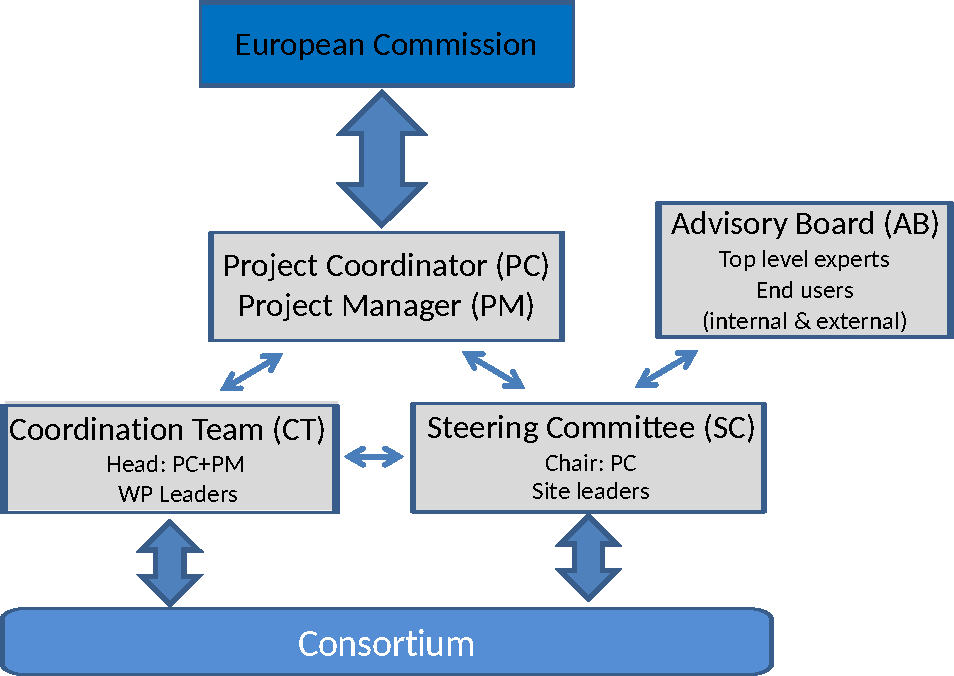
\includegraphics[width=0.75\textwidth]{management_structure.pdf}
  \caption{Management structure}
  \label{figure.management}
\end{figure}

The organisational structure, shown in the Figure~\ref{figure.management}, has been designed
to enable efficient coordination of the project --- the
development and evaluation of an Open Science toolkit
integrating several previously separated tools and software and
involving both academic actors and industrial stakeholders. It is jointly agreed on
by \TheProject consortium and adapted to its size and composition,
the tasks and duties of all partners involved.

We have designed the management structure and procedures to deal in a
flexible manner with the following challenges:
\begin{compactitem}
\item to integrate all consortium members and to mobilise their
  expertise, knowledge and networks at every stage of the project;
\item to give the maximum attention to the end-users needs and
  requirements;
\item to continuously involve expertise and knowledge of relevant
  stakeholders and their networks, and
\item to efficiently coordinate the project implementation in a
  collaborative environment and ensure its sustainability.
\end{compactitem}

The design has been largely adapted from that of OpenDreamKit which
has proved very effective for this type of project, with some
simplification as suggested by past experience:
\begin{itemize}
\item Suppression of the Quality Review Board: its role can
  effectively be subsumed by the steering committee; also the head of
  OpenDreamKit's Quality Review Board, Hans Fangohr, will carry over
  the accumulated experience and best practices, and the lessons
  learned from the OpenDreamKit quality review board will be shared
  within the BOSSEE consortium.
\item Suppression of the End User Group: as in OpenDreamKit, all
  participants are either end users themselves, or in close contact
  with such end users. To guarantee the effectiveness of this
  simplified structure, we include end users in the advisory board.
\end{itemize}


The coordinator acts as an intermediary between the Partners and
the European Commission. The coordinator will oversee the project
planning, monitor that execution is carried out in time and that
the objectives are achieved and closely interact with the project
officer for project monitoring and delivery of the performance
indicators.  The Project Manager will ensure  efficient day-to-day
management of the project, reporting, feedback to partners on
administrative, financial and legal issues, tracking of  resource
allocation and consumption, and communication inside and outside the
consortium.

The resources of all partners will be mobilised by decentralisation of
responsibilities through the assignment of leadership for work
packages. Clear distribution of tasks, efficient decision making
mechanisms and a sound financial management will safeguard the
achievement of the project's objectives.

\ifgrantagreement\else
\subsubsection{Milestones}
For a description of the milestones and their motivations see
Section~\ref{sec:milestones}; a tabulation of the milestones, which work packages
are involved, and a means of verification can be seen in Table~\ref{tab:milestonetable}.

\milestonetable
\fi

\subsubsection{Project roles}

%Project Coordinator and Project Manager can meet any time and at least
%twice a week.

The following bodies will form the organisational structure of the
\TheProject project : Coordination Team (CT), Steering Committee (SC),
Advisory Board (AB).%, End User Group (EUG) and Quality Review board (QRB).

\begin{description}
\item{\textbf{Coordination Team (CT)}} \nobreak\par
\textbf{Members:} The CT is composed of the Work Package leaders
and headed by the Project Coordinator, assisted by the Project
Manager.

\textbf{Responsibilities:} The CT is an executive body in charge of
the project implementation and monitoring.
It takes operational decisions necessary for the smooth execution of
the project.

\textbf{Tasks:}
\begin{compactenum}
\item Monitoring the timely execution of the tasks and achievement of
  the objectives;
\item Preparation of scientific and financial progress reports;
\item Controlling Work Package progress by assessing it through technical
  reports developed by the partners;
\item Making proposals to the Steering Committee of re-allocation of
  tasks, resources and financial needs for the fulfilment of the work
  plan;
\item Preparing the drafts and validating the project deliverables to
  be submitted to the Commission.
\end{compactenum}

\textbf{Meetings:} The coordination team will meet every 6 months.
If necessary, extra meetings will be arranged.

\item{\textbf{Steering Committee (SC)}}\nobreak\par

\textbf{Members:} The SC is chaired by the Project Coordinator
and includes one representative from each partner organisation.

\textbf{Responsibilities:} The SC is the decision-making body in
charge of the strategic orientation of the project.  It takes decisions on scientific
directions, re-allocation of resources, consortium
changes and intellectual property rights.

\textbf{Meetings:} Annual meetings. If necessary, extra-meetings
will be arranged.  Written minutes of each meeting will be produced,
which shall be the formal record of all decisions taken. A procedure
for comment and acceptance is proposed.

\textbf{Voting procedure:} The SC shall not deliberate until a quorum
of three-fourth (3/4) of all Members are present (possibly through
video-conference) or represented. Each Member shall have one vote. The
SC will work on consensual decisions as much as possible and resort to
voting only if unavoidable. Voting decisions shall be taken by a
majority of two-thirds (2/3) of votes with quorum two-thids (2/3) of
the whole set of members. Exceptional decisions (large changes to the
budget ($\geq$ 100k euros), evolution to the consortium, firing the
coordinator, resolving ambiguity about whether something is a hard
question) shall be taken by a majority of three-fourth (3/4) of votes
with quorum three-fourth (3/4) of the whole set of members. Votes can
be electronic.

\item{\textbf{Advisory board (AB)}} \nobreak\par

  \textbf{Members:} top level experts and end-users from partner and
  external organisations, from a variety of disciplines and both from
  academic and industrial sector. Together, they have a deep
  understanding of both market and technical problems, and an
  awareness of opportunities

  \textbf{Responsibilities:} to give an independent opinion on
  steering, scientific and innovation matters, in order to guaranty
  quality implementation of the project, adequateness to the end-users
  needs, efficient innovation management, and project sustainability.

  % \textbf{Tasks:} to control the project execution from the point of
  % view of the end user needs and requirements, to test the tool and to
  % detect its potential shortcomings at the early stages, to propose
  % adaptation measures.

  \textbf{Meetings:} at the request of the Steering Committee, including attending annual project meetings.
\end{description}

\subsubsection{Project management tools and procedures}

Project partners and management bodies will communicate through
a dedicated project web platform, maintained by the Project
Manager. WP leaders will monitor progress of
participants of their WP at least monthly, and participants will inform their WP
leaders when problems are encountered. Major problems will be
discussed in (teleconference) meetings with the Project Coordinator
and Project Manager. Each WP leader will be free to organise
extra meetings with WP partners, if necessary. Scientific and
financial progress reports will be collected, assembled and
transmitted to the Project Coordinator by the WP leaders through the
web platform. On basis of the Progress Reports, the Coordination Team
will monitor progress of the project, identify bottlenecks and find
solutions for these problems. Where needed, adaptations to the project
plan will be made, with the aim of ensuring the delivery of the project
results as agreed with the EC. Major adaptations need to be approved
by the Steering Committee.

The Coordination Team, will ensure efficient innovation management.
They will carefully monitor new opportunities in order to suggest, if
necessary, to new directions to the Steering Committee. For legal
aspects, the latter will have a feedback from legal officers from the
Coordinator’s European affairs office,
specialised in Intellectual Property.

Our management structure and procedures will ensure that our network
of partners from both academic and industrial sectors is focused at
achieving the promised tasks and deliverables, efficiently managing
the innovation process and largely opening the developed tools,
insights and services to the EOSC and its final users.
The partners will sign a Consortium Agreement, in which operational
rules and decision making procedures will be laid down.

\emph{CONFLICT RESOLUTION} - For the cases where contentious decisions
need to be made, or conflicts are arising which cannot be solved bilaterally,
steps to prevent further escalation and procedures to resolve disputes
and decision-making procedures are laid down in the Consortium Agreement.
In case of conflicts or a needed decision in a task or work package,
the WP Leader shall resolve the conflict and agree on a solution or decision.
If a solution of the conflict cannot be found or if a Party does not accept
the proposed solution, the issue must be forwarded to the Steering committee (SC),
which in its turn will try to resolve the issue together with the conflicting parties
within 10 working days. If no agreement can be reached, the Project Coordinator (PC) can
base its decision on the 2/3 majority vote of the SC or take a different decision.
In any case, the Coordinator will take the final decision. All parties will make
efforts that decisions are resolved at a level as low as possible.

\subsubsection{Quality and Innovation management}

\TheProject Project Quality Management will ensure that
the project meets a high quality level as well as satisfying the EU commission
requirements. The basic approach to quality management is compatible with the
International Project Management standards and guidelines (PMI).

\begin{itemize}
\item Quality planning: internal standards from participants and national and international standards and
regulatory requirements will be considered to create the quality metric.
\item Quality control: the overall project performance will be evaluated on a regular basis to provide
confidence that the project satisfies the expectation and EU provisions.
\item Quality assurance: specific project results will be monitored to determine if they comply with
expectations and eliminate causes of unsatisfactory performance. To this aim, deliverables have been
planned to give the necessary information and evidence that quality standards have been achieved.
\end{itemize}

In the context of the Responsible Research Innovation paradigm promoted by the European Commission in
the H2020 framework, \TheProject is willing to respond to societal desirability and societal acceptability
question identifying new opportunities in the Open Science hub through innovation that is in the public
interest. \TheProject consortium recognises innovation as an essential element for driving business growth
and maintaining competitive advantage. The innovation management work will prevent that \TheProject
results suffer from missing expected functionalities, which would lead to user dissatisfaction, and will
ensure that the ethical and societal aspects are incorporated into the design process from the beginning.

\subsubsection{Risks and risk management strategy}\label{sec:risks}

The risk in the project execution as planned is carefully assessed and
managed. We base our plans on long standing experience, and we bring
together the world's experts in the relevant tools and techniques.

A key feature of this project is the involvement of a wide set of
partners from multiple domains. While this ensures complementary
coverage of a wide set of skills and provides robustness in different
ways, we will have to ensure that all the partners work together as
a closely knit team.

Our open source approach means that all our code and outputs
will be open and visible to anybody at sites like GitHub and Bitbucket
throughout the project. It is common for some users to run the latest
development versions of computational and infrastructure software, thus
beta-testing code between major releases.
This reduces the risk of developing software which people won't use:
where our design decision or technical approaches are
controversial, this will be detected early by those users, giving the
consortium useful feedback to consider.

As part of the Management Work Package, and with support from the
Coordination Team, the project coordinator will maintain and regularly
update a Risk Management Plan; at the end of each Reporting Period,
this updated plan will be included in the project's Technical Report.
It will identify and categorise all
potential strategic risks (legal, financial, human resources risks, etc.)
to the successful delivery of the project, their probability and impact.
For each risk area, mechanisms for risk mitigation will be identified
and contingency actions will be proposed.

Risks will be evaluated in terms of project goals and objectives,
according to the following four steps:
\begin{enumerate}
\item Identification of risks using a structured and rational approach to
ensure that all areas are addressed.
\item Quantitative assessment and ranking of the risks.
\item Definition of procedure to reduce (or minimize) risk.
\item Monitoring and management of risks throughout the project life
with milestone review and reassessment.
\end{enumerate}

Finally, as reported above, a conflict resolution mechanism will be put in place,
whereby decision making divergence and conflicts that cannot be solved
at the Steeing Committee (SC) level will be submitted to the Coordinator. The
mediation and resolution process used is the following:
\begin{itemize}
\item Case presented by the involved parties.
\item Development of a fact-based and neutral report by the coordinator
to be provided to the conflicting parties and SC.
\item Final decision to resolve the conflict made by SC.
\end{itemize}

\ifgrantagreement\else
An initial risk assessment appears as Figure~\ref{risk-table}.

\TOWRITE{ALL}{risk about EOSC integration}

\begin{figure}
\begin{center}
\begin{tabular}{|m{.2\textwidth}|m{.12\textwidth}|m{.58\textwidth}|}\hline
  Risk & Level with / without mitigation & Mitigation measures
  \\\hline

   \multicolumn{3}{|c|}{
    \textit{General technical / scientific risks}
   }
   \\\hline

  Implementing infrastructure that does not match the needs of end users & High/Low &
  Many of the members of the consortium are themselves end-users with
  a diverse range of needs and points of views; hence the design of
  the proposal and the governance of the project is naturally steered
  by demand; besides, because we provide a toolkit, users have the
  flexibility to adapt the infrastructure to their needs.\\\hline

  Lack of predictability for tasks that are pursued jointly with
  the community & Medium/Low &
  The PI's have a strong experience managing community-developed
  projects where the execution of tasks depends on the availability of
  partners. Some tasks may end up requiring more manpower from
  \TheProject to be completed on time, while others may be entirely
  taken care of by the community. Reallocating tasks and redefining
  work plans is common practice needed to cater for a
  fast evolving context. Such random factors will be averaged out over
  the large number of independent tasks.\\\hline

  Reliance on external software components & Medium/Low & The non trivial
  software components \TheProject relies on are open source. Most are
  very mature
  and supported by an active community, which offers strong long run
  guarantees. The other components could be replaced by alternatives, or
  worst comes to worst, taken over by the participants.
  \\\hline

%  \multicolumn{3}{|c|}{
%    \textit{Use-case risks}
%  }
%  \\\hline
%
%  & & \TOWRITE{WP4}{Risks related to use-cases in WP4}
%  \\\hline

  \multicolumn{3}{|c|}{
    \textit{Management risks}
  }
  \\\hline

  Recruitment of highly qualified staff & High/Medium &

  Great care was taken coordinating with currently running projects to
  rehire personnel with strong track record, and identifying pool of
  candidates to hire from, notably in the developers community of
  software related to the project. This was favored by the partners'
  long history of training and outreach activities. In addition, we
  have a critical mass of qualified staff in the project enabling us
  to train new recruits.

 \\\hline

  Different groups not forming effective team & Medium/Low & Long
  track record of working collaboratively on code across multiple
  sites. Aggressive planning of project meetings, workshops and
  one-to-one partner visits to facilitate most effective teamwork,
  combining face-to-face time at one site with remote
  collaboration.\\\hline
  % this also justifies our generous travel budget.

  Partner leaves the consortium & Low/High & If the GA requires a replacement
  in order to achieve the project's objectives, the consortium will invite a new
  relevant partner in. If a replacement is not necessary, the resources and tasks
  of the departing partner will be reallocated to the alternative ones within the
  consortium.
  \\\hline

  \multicolumn{3}{|c|}{
    \textit{Dissemination risks}
  }
  \\\hline

  Impact of dissemination activities is lower than planned. & Low/Medium &

  Partners in the consortium have a proven track record at community
  building, training, dissemination, social media communication, and
  outreach, which reduces the risk. The Project Coordinator
  will monitor impact of all dissemination activities. If a deficiency is identified, the consortium
  will propose relevant corrective actions.\\\hline

  \end{tabular}
\end{center}
\caption{\label{risk-table}Initial Risk Assessment}
\end{figure}
\fi
%\TOWRITE{NT/Eugenia}{Impredictability}

%\includegraphics[width=.94\textwidth]{Pictures/Impact-img1.png}

%   But: since Open Source softwares are freely accessible, security
%   and privacy issues are a concern. Anytime a resource is shared,
%   there is greater risk of unauthorised access and contaminated data.
%   Providers must demonstrate security solutions, which should include
%   physical security controlling access to the facility and protection
%   of user data from corruption and cyber attacks.}


\TOWRITE{ALL}{
  Add a paragraph about data management plan. What data will we produce, which data is available from the
  start, how do we handle it...
}

%  LocalWords:  mgt Paris-Sud UPSud Thiery Sage-Combinat decentralisation textwidth hline
%  LocalWords:  textwidth Jupyter slmhnlnhfnhs hsfhs ghshsh includegraphics unauthorised

%%% Local Variables:
%%% mode: latex
%%% TeX-master: "proposal"
%%% End:
%  LocalWords:  TOWRITE subsubsection organisational compactenum ipr Impredictability
%  LocalWords:  textbf nobreak smallbreak


\draftpage
\subsection{Consortium as a Whole}
%\TO WRITE{ALL}{Proofread 3.4 consortium pass 2 [Done by Hans]}
%remove this, as we have more pressing things left.

\eucommentary{\begin{compactitem}
\item
Describe the consortium. How will it match the project's objectives?
How do the members complement one another (and cover the value chain,
where appropriate)? In what way does each of them contribute to the
project? How will they be able to work effectively together?
\item
If applicable, describe the industrial/commercial involvement in the
project to ensure exploitation of the results and explain why this is
consistent with and will help to achieve the specific measures which
are proposed for exploitation of the results of the project (see section 2.3).
\item
Other countries: If one or more of the participants requesting EU funding
is based in a country that is not automatically eligible for such funding
(entities from Member States of the EU, from Associated Countries and
from one of the countries in the exhaustive list included in General
Annex A of the work programme are automatically eligible for EU funding),
 explain why the participation of the entity in question is essential to
 carrying out the project
\end{compactitem}
}

The \TheProject consortium spans the broad spectrum of actors required
for successfully developing an apt and easy-to-navigate sustainable service
accessible through the EOSC hub catering to the needs of the European
scientific community. It is composed of four academic institutions, four research
centers, one e-Infrastructure federation, and two SMEs based in six different countries (Norway, France,
Netherlands, Germany, Poland, Switzerland).
The Consortium ensures a critical mass of scientific expertise and excellence
in key areas (astronomy, geosciences, health sciences,
mathematics, photon science, education) with research organisations and SMEs of recognised
 international reputation. Namely, \TheProject consortium brings in:
\begin{compactitem}
\item A set of use cases that cover several application domains and users, and that impose very diverse
requirements on EOSC infrastructure (European XFEL, CDS ASTRO, UiO, INSERM, Paris Sud);
\item Lead developers in the Jupyter Ecosystem, including IPython, the Jupyter Notebook, JupyterLab,
JupyterHub, Binder, MyBinder.org, Jupyter Widgets located at Simula, European XFEL, QuantStack, and
WildTreeTech,
as referenced in section \ref{jupyter-ecosystem}.
\item Experts and major promoters of the Jupyter collaborative user interfaces for interactive and exploratory
computing in a variety of scientific domains (Centre de Donnees
astronomiques de Strasbourg, European XFEL,
INSERM, QuantStack, Paris-Sud, \'Ecole Polytechnique, Silesia,
University of Oslo).
\item A long experience and proven track record of success with large and complex collaborative projects,
including
European E-Infrastructure projects (XFEL, Simula, UPSud, Silesia),
projects focused on large-scale infrastructures and large experimental services (EGI, XFEL),
as well as experience in running large scale open source projects (Jupyter project).
\item A comprehensive range of skill sets and competencies in several relevant domains, from applied
research to standardisation to business
analysis.
\end{compactitem}

The consortium has developed through collaborations and common interests over recent years.
Some partners have been working together on different aspects of Jupyter
and software for education for many years (European XFEL, QuantStack, Simula, Wild Tree Tech).
Meanwhile, others joined together during a previous successful
H2020 European Research Infrastructure project OpenDreamKit \#676541 (European XFEL,
Paris-Sud, Silesia, Simula).
OpenDreamKit's review meetings and participation to H2020
E-infrastructure events, as well as community Jupyter workshops (organized by
e.g. by \'Ecole Polytechnique, Paris-Sud, Simula, UiO) led to
connections with UiO, INSERM, and EGI, and to collaborations such as a
prototype deployment of Binder on EGI's infrastructure. The connection
with CDS ASTRO grew out of a workshop coorganized back in 2013 by
Paris-Sud on mathematical databases, where CDS's head Françoise Genova
was invited speaker; this later led to her joining OpenDreamKit's
Advisory Board.

Finally, we note that the project partners are long time passionate
advocates of Open Science;
building on highly successful past experience with OpenDreamKit, they
\emph{have chosen to write this proposal fully in the open} on GitHub
(\href{http://github.com/bossee-project/proposal}{http://github.com/bossee-project/proposal}) for maximum transparency
and engagement of the community.
We have used the same open source collaboration tools and practices
as the Open Source Open Science community.

In addition to the joint planning and writing period for this
proposal, the project partners have been interacting through a number of
other activities, including:

\begin{enumerate}
\item Joint software development
  \begin{itemize}
  \item Jupyter Notebook (\site{XFEL}, \site{SRL}, \site{WTT}, \site{QS})
  \item Jupyter Widgets (\site{QS}, \site{SIL}, \site{UPSUD}, \site{SRL})
  \item Binder and repo2docker (\site{SRL}, \site{WTT})
  \item thebelab (\site{QS}, \site{SRL}, \site{UPSUD})
  \item nbval (\site{XFEL}, \site{SRL})
  \end{itemize}

\item Joint projects
  \begin{itemize}
  \item \href{http://opendreamkit.org}{OpenDreamKit} (\site{XFEL}, \site{SRL}, \site{UPSUD}, \site{SIL})
  \item PaNOSC (\site{EGI}, \site{XFEL})
  \item Computing in high school science education - iCSE4school, Erasmus+ Strategic Partnerships,
  (\site{SRL}, \site{SIL}), 2014-2017
  \item Computers in Science Education:iCSE (\site{SIL}, \site{UIO}), funded by EFS, 2011-2014.
    \end{itemize}

\item Joint publications
  \begin{itemize}
  \item \emph{Jupyter Notebooks -- a publishing format for
      reproducible computational workflows} \cite{Kluyver2016} (\site{XFEL}, \site{SRL}, \site{QS})
  \end{itemize}

\item Collaboration
  \begin{itemize}
  \item MyBinder for teaching and reproducibility (\site{XFEL}, \site{SRL}, \site{WTT})
  \item Widgets for computational science (\site{XFEL}, \site{QS}, \site{SIL})
  \item OpenGATE, Monte Carlo platform for medical applications (
    \site{INSERM}, \site{UPSUD})
  \item Life Science Grid Community (\site{EGI}, \site{INSERM})
  \item JupyterDays events organised at \'Ecole Polytechnique, Paris-Sud,
  and other sites, with participation from other sites
  (\site{CDS}, \site{EP}, \site{UPSUD}, \site{SRL}).
  \item Research Bazaar workshops on Jupyter, Binder, and reproducibility
    (\site{SRL}, \site{UIO})
 \end{itemize}
\end{enumerate}

Table \ref{tab:collaboration} shows a summary of the links
between partners.

\TOWRITE{ALL}{Add previous collaborations}

% joint software/database development
% Jupyter Project software

\jointsoft{XFEL,SRL}
\jointsoft{WTT,SRL}
\jointsoft{WTT,XFEL}

% Binder
\jointsoft{SRL,WTT}

% k3d
\jointsoft{SIL,SRL}
\jointsoft{SIL,XFEL}
\jointsoft{SRL,XFEL}

% nbval
\jointsoft{XFEL,SRL}

%%s

% OpenDreamKit: UPSUD, SIL, XFEL, SRL
\jointproj{XFEL,UPSUD}
\jointproj{XFEL,SRL}
\jointproj{XFEL,SIL}

\jointproj{UPSUD,SRL}
\jointproj{UPSUD,SIL}

\jointproj{SRL,SIL}
\jointproj{UIO,SIL}

% jupyterhub deployment
\jointproj{EP,UPSUD}

% Binder persistent storage
\jointproj{UPSUD,WTT}
\jointproj{EP,WTT}

% xeus-cling
\jointsoft{QS,EP}
\jointsoft{QS,UPSUD}

% prototype Binder deployment on EGI
\jointproj{Simula, EGI}

% panosc
\jointproj{XFEL,EGI}

% Jupyter project publication ? XXX TIM

% Binder
\jointsoft{SRL,WTT}

% research bazaar
\jointproj{SRL,UIO}

% JupyterDays Orsay + ecole
\jointproj{UPSUD,EP}
\jointproj{UPSUD,CDS}
\jointproj{UPSUD,SRL}
\jointproj{UPSUD,QS}

\jointproj{EP,CDS}
\jointproj{EP,SRL}
\jointproj{EP,QS}

% \jointproj{CDS,SRL}
% \jointproj{CDS,QS}

% \jointproj{SRL,QS}

% OpenGATE
\jointproj{INSERM,UPSUD}

% Life Sciences Grid
\jointproj{INSERM,EGI}

% \jointpub{A,B} % some publication

%joint supervision
% \jointsup{A,B} %

%joint organization
% \jointorga{A,B} % some org
% \jointorga{SA,UJF} % PASCO'15

% joint publications
% \jointpub{A,B} % some publication

% Jupyter publication
\jointpub{SRL,XFEL}
\jointpub{SRL,QS}
\jointpub{XFEL,QS}

\coherencetable[swsites]

%%% Local Variables:
%%% mode: latex
%%% TeX-master: "proposal"
%%% End:

%%% Local Variables:
%%% mode: latex
%%% TeX-master: "proposal"
%%% End:

\draftpage

\subsection{Resources to be Committed}\label{sec:resources}
%
%\eucommentary{Please provide the following:
%\begin{compactitem}
%\item
%a table showing number of person/months required (table 3.4a)
%\item
%a table showing 'other direct costs' (table 3.4b) for participants where
%those costs exceed 15\% of the personnel costs (according to the budget
%table in section 3 of the administrative proposal forms)
%\end{compactitem}}
%
\TheProject applies for a total budget of \textbf{\euro 5,927,192.50} as the amount
required achieving the objectives. The total budget is described in the subsequent
sections together with the staff effort necessary to implement the action (Table 3.4.1).
The necessary physical resources, the quantities of each and when they would be
needed has been carefully determined on the base of the following criteria:

\begin{enumerate}

\item \textbf{Historical information} the partners involved are well experienced in the
Jupyter development, software for education, processing and scale-up; past experiences
from each partner has been taken into consideration to evaluate what, and in what
quantities, different resources will be needed in the project.
\item \textbf{Work plan structure} the deliverables and milestones identified in the project work plan.
\item \textbf{The inputs necessary to resource planning}; further, the timetable of activities has helped to identify when each resource will be needed in the project.
\item \textbf{Resource pool description} the resources available in the consortium have
been carefully analysed in order to avoid any duplicating of existing resources
and allocate efficiently and effectively the resources necessary.
\item \textbf{Cost estimating}  The approximated costs of the resources needed to
complete successfully the project activities has been estimated on the base
of: a) Resource planning results, b) Activity duration estimation (Gantt and effort form),
c) Commercially available data on durables and consumables needed,
d) Preliminary Risk Assessments.
The financial allocation among the 11 partners reflects the tasks committed by each partner
and the collaborative nature of the project itself. On the whole, the financial allocation is
well-balanced and homogeneous.
\end{enumerate}

\subsubsection{Management Level Description of Resources and Budget}
\label{sect:budget-details}

\paragraph{Staff efforts}

\eucommentary{Please indicate the number of person/months over the whole
duration of the planned work, for each work package, for each participant.
Identify the work-package leader for each WP by showing the relevant
person-month figure in bold.}

The \TheProject project is gathering sites with core developers from
the Jupyter project and history in open source software development,
and brings them together with domain specialists from a range of
domains. The major investment of the project is in software
development, which is realised through person time and displayed in table~3.4.1.

\ifgrantagreement.\else{} %

\wpfig[label=fig:staffeffort,caption=Summary of Staff Efforts]
\fi

\paragraph{Travel, dissemination, and outreach}

The nature of this proposal -- of providing a framework that allows
design and deployment of innovative services -- means that the project
has the potential to have high impact for EOSC. At the same time, it
requires input from and engagement with a significant number of
stakeholders, including potential users of the services such as
scientists, developers of other services and other EOSC-funded
projects, other open science software projects, and the developing
EOSC itself. Consequently, requirements capture, networking, feedback,
training and education workshops and outreach activities are all
important, and the second highest cost for this project.

\subparagraph{Guidelines for travel and dissemination}
\label{sect:budget-details-travel}

We use the following guidelines for expected travel expenses:
\euro{2500} for attendance of a typical one week international
conference outside Europe (including travel, subsistence,
accommodation and registration), \euro{1250} for a corresponding
conference in Europe, \euro{750} for a one-week visit of a project
partner, for instance for coding sprints and one-to-one
research visits. We expect a similar cost per week while hosting
visitors. For the half-yearly project meetings, we expect on average a
cost of \euro{500} for travel, accommodation and subsistence.

Anticipated activities:

\begin{enumerate}
\item \emph{Project meetings}: For the 9 project meetings that take place every 6 months, we expect
the PI to attend all of them (cost of 9 * 500 = \euro{4500}). For
a researcher, we also expect that they attend all such project meetings
(\euro{4500}).

\item \emph{Hosting visitors}: We expect that the site spends \euro{2000} per year to host
external visitors contributing to the project (total \euro{8000}).

\item \emph{Site visits}: We expect the researcher to carry out 3 one-week visits to other sites
(each at \euro{750}) every year, totalling 3 * 4 * 750 = \euro{9000}
over 4 years).

\item
\emph{Conference dissemination}: We expect the researcher to attend on average 1
international conference and 1 European meeting per year (cost of 4 *
2500 + 4 * 1250 = \euro{15000}) and the investigator to attend the
equivalent of one international or two
European gatherings (totals \euro{10000}).
\end{enumerate}

Where there are multiple investigators per site, they will share the
travel and associated costs outlined above. Where there are multiple
researchers, or researchers not employed for the full 48 months, the
travel budget is adapted accordingly.



\subparagraph{Guidelines for outreach costs}

\label{sect:budget-outreach-publication-charges}
\emph{Publication charges}: We also request \euro{3000} per partner to pay for open
access publication charges.  (Some partners have other means do pay
these costs, and for them these are not needed.)

\label{sect:budget-outreach-workshops}
\emph{Workshops}: We request funds for dissemination and outreach
activities such as workshops that facilitate community building,
provide training and disseminate best practice and encourages
sustained contributions of the community to the project and beyond the
lifetime of the funding. For a one-week workshop that we organise,
we will typically use meeting rooms of the project partners to minimise
cost, and assume a cost of 400 EUR per participant to provide location
and subsidise accommodation and catering for attendees. A workshop for 10 people
will thus cost about \euro{4000}. Participants
donate their time and need to fund their travel from other sources. By
partially contributing to the attendance cost, we hope to enable PhD
students to engage with the project and expect positive effects on the
sustainability of the activities, by embedding the tools and knowledge
with the next generation of scientists.

Details are given in the tables below and in the work packages.

\bigskip



 \subsubsection{Resource summaries for consortium member sites}
 \label{resources.summary}

 %%%%%%%%%%%%%%%%%%%%%%%%%%%%%%%%%%%%%%%%%%%%%%%%%%%%%%%%%%%%%%%%
 %
 % Guidelines for completion of partner specific resource summary:
 %
 %
 % Please explain how many person months for each person are
 % requested. Say who is the local lead. Say anything that helps to
 % understand why people are recruited as you plan, in particular if
 % this deviates from having one research for 48 months.  We can also
 % use this bit of the proposal (and the table, see below) to address
 % any other unusual arrangements.
 %
 %
 % The table should contain all non-staff costs (the EU requests that
 % this table must be present if the non-staff costs exceed
 % 15% of the total cost, but it is good practice and will show
 % openness and transparency that we show the data for all partners).
 %
 % Link back from the table to the work packages and tasks for which
 % the expenses are required. Add information that makes it easier to
 % understand why the expenses are justified.
 %
 %     To refer to a task in a work package, use "\taskref{WP-ID}{TASK-ID}" where
 %     WP-ID is the ID of the work package:
 %        WP#: WP-ID - full title
 %        ----------------------
 %        WP1: 'management' - Management
 %        WP2: 'community' - Community Building and Engagement
 %        WP3: 'component-architecture' - Component Architecture
 %        WP4: 'UI' - User interfaces
 %        WP5: 'hpc' - High Performance Computing
 %        WP6: 'dksbases' - Data/Knowledge/Software-Bases
 %        WP7: 'social-aspects' - Social Aspects
 %        WP8: 'dissem' - Dissemination
 %
 %
 %     and "TASK-ID" is the ID of the task. You can set this using
 %
 %       \begin{task}[id=TASK-ID,title=Math Search Engine,lead=JU,PM=10,lead=JU]
 %
 %     To refer to deliverables, use "\delivref{WP-ID}{DELIV-ID}" where DELIV-ID is
 %     the ID of the deliverable that can be set like this:
 %
 %       \begin{wpdeliv}[due=36,id=DELIV-ID,dissem=PU,nature=DEM]
 %           {Exploratory support for semantic-aware interactive widgets providing views on objects
 %           represented and or in databases}
 %       \end{wpdeliv}
 %
 %
 % The table is pre-populated with entries most sites are likely
 % to need. If a line does not apply to you, just delete it. If you need
 % an extra line, then add it. Use common sense: the number of rows should not
 % be very big, but at the same time it is useful to give some breakdown/explanation
 % of costs.
 %
 %
 % Eventually, try to create you entry similar in style to the others.
 % (The Southampton entry is fully populated, so use this as guidance
 % if in doubt.)
 %
 %
 %%%%%%%%%%%%%%%%%%%%%%%%%%%%%%%%%%%%%%%%%%%%%%%%%%%%%%%%%%%%%%%%

 In this section we briefly describe the requested resources. See the
 participant descriptions in the description of the consortium for the
 specific role of each member.

 Some partners do not require all the costs outlined above in
 section~\ref{sect:budget-details} and have accordingly reduced their
 requirements below.  \bigskip


 %%%%%%%%%%%%%%%%%%%%%%%%%%%%%%%%%%%%%%%%%%%%%%%%%%%%%%%%%%%%%%%%%%%%%%%%%%%%%%
 \paragraph{Resources Simula Research Laboratory}

 % See line 122 in
 % https://docs.google.com/spreadsheets/d/1vXm5Z2pIWIf6UCWWkXDQ4Fti8PM6xBnpXNhehUAKmuk/edit#gid=322027044 for details
 %

 % Travel
 % Assume PI (50%) and 2 FTE researchers
 %
 % Project meetings:
 % 3 * 9000 = 27,000
 % Hosting visitors = 8000
 % Site visits 2 * 9000 = 18000
 % Conference dissemination = 2 * 15000 + 1 * 10000 = 40000
 %
 % Publication costs: 3000
 % Workshops: 4 x 10 people = 16,000
 %
 %
 %
 % Cloud computing
 % financial audit
 % laptops

 \site{SRL} requests 124 person months to provide the effort required.

 \bigskip
 \begin{table}[H]
 \begin{tabular}{|r|r|p{8.5cm}|}
   \hline
   \textbf{\site{SRL}} & \textbf{Cost (\euro)} & \textbf{Justification} \\\hline
   \textbf{Travel} &  79500 & Travel for PI and 2 researchers (see
                              \ref{sect:budget-details-travel})\\\hline
   \textbf{Workshops} & 16000 & Workshops (40 attendees in total) (see \ref{sect:budget-details-travel})\\\hline
   \textbf{Publication charges}
                       &  3000 & Open access publication charges (see \ref{sect:budget-outreach-publication-charges})\\\hline
 %%\textbf{Equipment}
 %%  &   0 &  \\\hline    %\taskref{WP-ID}{TASK-ID}
 \textbf{Other goods and services}
                        &  3500 & Financial audit \\\hline
   & 7500 & Consumables (3 High Performance laptops for workshops,
            sprints, dissemination )  \\\hline
 \textbf{Total}
  & 109500\\\cline{1-2}
 \end{tabular}
 \caption{Overview: Non-staff resources to be committed at Simula
   Research Laboratory
   (all in \texteuro)}\vspace*{-1em}
 \end{table}

%%  %%%%%%%%%%%%%%%%%%%%%%%%%%%%%%%%%%%%%%%%%%%%%%%%%%%%%%%%%%%%%%%%%%%%%%%%%%%%%%
%%  \paragraph{Resources Facility}
%%
%%  \site{...} requests
%%  X person months for
%%
%%  \taskref{wpid}{taskid}
%%
%%
%%  \bigskip
%%  \begin{table}[H]
%%  \begin{tabular}{|r|r|p{8.5cm}|}
%%  \hline
%%  \textbf{2: \site{SRL}} & \textbf{Cost (\euro)} & \textbf{Justification} \\\hline
%%  \textbf{Travel}
%%    &  XXX & Travel (see  \ref{sect:budget-details-travel})\\\hline
%%  \textbf{Publication charges}
%%    &   XXX & Open access publication charges (see \ref{sect:budget-outreach-publication-charges})\\\hline
%%  %%\textbf{Equipment}
%%  %%  &   0 &  \\\hline    %\taskref{WP-ID}{TASK-ID}
%%  \textbf{Other goods and services}
%%    & XXX &
%%   \\\hline   %\taskref{WP-ID}{TASK-ID} \delivref{WP-ID}{DELIV-ID}
%%  \textbf{Total}
%%   & XXX\\\cline{1-2}
%%  \end{tabular}
%%  \caption{Overview: Non-staff resources to be committed at CNRS (all in \texteuro)}\vspace*{-1em}
%%  \end{table}
%%



  %%%%%%%%%%%%%%%%%%%%%%%%%%%%%%%%%%%%%%%%%%%%%%%%%%%%%%%%%%%%%%%%%%%%%%%%%%%%%%

\paragraph{Resources CDS Astro}

\site{CDS} requests 18 person months to provide the effort required.

\bigskip
\begin{table}[H]
\begin{tabular}{|r|r|p{8.5cm}|}
  \hline
  \textbf{\site{CDS}} & \textbf{Cost (\euro)} & \textbf{Justification} \\\hline
  \textbf{Travel} &  13750 & Travel for PI and $\approx$0.4 researchers (see
                             \ref{sect:budget-details-travel})\\\hline
  \textbf{Workshops} &  4000 & Workshop (10 attendees in total) (see  \ref{sect:budget-details-travel})\\\hline
  \textbf{Publication charges}
                      &  3000 & Open access publication charges (see \ref{sect:budget-outreach-publication-charges})\\\hline
%%\textbf{Equipment}
%%  &   0 &  \\\hline    %\taskref{WP-ID}{TASK-ID}
\textbf{Total}
 & 20750 \\\cline{1-2}
\end{tabular}
\caption{Overview: Non-staff resources to be committed at CDS (all in \texteuro)}\vspace*{-1em}
\end{table}


\paragraph{Resources \'Ecole Polytechnique}

\site{EP} requests 52 person months to provide the effort required.

\bigskip
\begin{table}[H]
\begin{tabular}{|r|r|p{8.5cm}|}
  \hline
  \textbf{\site{EP}} & \textbf{Cost (\euro)} & \textbf{Justification} \\\hline
  \textbf{Travel} &  45000 & Travel for PI and 1 researchers (see
                             \ref{sect:budget-details-travel})\\\hline

\textbf{Workshops} & 8000 & Workshop (20 attendees in total) (see  \ref{sect:budget-details-travel})\\\hline
  \textbf{Publication charges}
                      &  3000 & Open access publication charges (see \ref{sect:budget-outreach-publication-charges})\\\hline
%%\textbf{Equipment}
%%  &   0 &  \\\hline    %\taskref{WP-ID}{TASK-ID}
  \textbf{Other goods and services}
                        &  5000 & Financial audit \\\hline
\textbf{Total}
 & 61000 \\\cline{1-2}
\end{tabular}
\caption{Overview: Non-staff resources to be committed at \'Ecole Polytechnique
  (all in \texteuro)}\vspace*{-1em}
\end{table}


\paragraph{Resources EGI}

\site{EGI} requests 24 person months to provide the effort required.

\bigskip
\begin{table}[H]
\begin{tabular}{|r|r|p{8.5cm}|}
  \hline
  \textbf{\site{EGI}} & \textbf{Cost (\euro)} & \textbf{Justification} \\\hline
  \textbf{Travel} &  20750 & Travel for PI and 0.5 researchers (see
                             \ref{sect:budget-details-travel})\\\hline
%%\textbf{Equipment}
%% &   0 &  \\\hline    %\taskref{WP-ID}{TASK-ID}
\textbf{Other goods and services}
                      &  4500 & Financial audit \\\hline
                      & 180000 & Cloud computing (180k; 5k/month) for
                                 operation of services including \taskref{eosc}{eu-binder}.
   \\\hline
\textbf{Total}
 & 200750 \\\cline{1-2}
\end{tabular}
\caption{Overview: Non-staff resources to be committed at EGI (all in \texteuro)}\vspace*{-1em}
\end{table}


\paragraph{Resources European XFEL}

\site{XFEL} requests 123 person months to provide the effort required.

\bigskip
\begin{table}[H]
\begin{tabular}{|r|r|p{8.5cm}|}
  \hline
  \textbf{\site{XFEL}} & \textbf{Cost (\euro)} & \textbf{Justification} \\\hline
  \textbf{Travel} &  79500 & Travel for PI and 2 researchers (see
                             \ref{sect:budget-details-travel})\\\hline
  \textbf{Workshops} &  16000 & Workshops (40 attendees in total) (see  \ref{sect:budget-details-travel})\\\hline
  \textbf{Publication charges}
                      &  3000 & Open access publication charges (see \ref{sect:budget-outreach-publication-charges})\\\hline
%%\textbf{Equipment}
%%  &   0 &  \\\hline    %\taskref{WP-ID}{TASK-ID}
\textbf{Other goods and services}
                      &  6500 & Financial audit \\\hline
  & 7500 & Consumables (3 High Performance laptops for workshops,
           sprints, dissemination )  \\\hline
\textbf{Total}
 & 112500 \\\cline{1-2}
\end{tabular}
\caption{Overview: Non-staff resources to be committed at European XFEL (all in \texteuro)}\vspace*{-1em}
\end{table}


\paragraph{Resources INSERM}

\site{INSERM} requests 39 person months to provide the effort required.

\bigskip
\begin{table}[H]
\begin{tabular}{|r|r|p{8.5cm}|}
  \hline
  \textbf{\site{INSERM}} & \textbf{Cost (\euro)} & \textbf{Justification} \\\hline
  \textbf{Travel} &  37300 & Travel for PI and $\approx$0.8 researchers (see
                             \ref{sect:budget-details-travel})\\\hline

\textbf{Workshops} & 4000 & Workshop (10 attendees in total) (see  \ref{sect:budget-details-travel})\\\hline
  \textbf{Publication charges}
                      &  3000 & Open access publication charges (see \ref{sect:budget-outreach-publication-charges})\\\hline
%%\textbf{Equipment}
%%  &   0 &  \\\hline    %\taskref{WP-ID}{TASK-ID}
  \textbf{Other goods and services}
%                        &  3500 & Financial audit \\\hline
  & 2500 & Consumables (1 High Performance laptop for workshops,
           sprints, dissemination)  \\\hline
\textbf{Total}
 & 46800 \\\cline{1-2}
\end{tabular}
\caption{Overview: Non-staff resources to be committed at INSERM
  (all in \texteuro)}\vspace*{-1em}
\end{table}


\paragraph{Resources QuantStack}

\site{QS} requests 48 person months to provide the effort required.

\bigskip
\begin{table}[H]
\begin{tabular}{|r|r|p{8.5cm}|}
  \hline
  \textbf{\site{QS}} & \textbf{Cost (\euro)} & \textbf{Justification} \\\hline
  \textbf{Travel} &  51000 & Travel for PI and 1 researcher (see
                             \ref{sect:budget-details-travel})\\\hline
  \textbf{Workshops} &  8000 & Workshops (40 attendees in total) (see  \ref{sect:budget-details-travel})\\\hline
  \textbf{Publication charges}
                      &  3000 & Open access publication charges (see \ref{sect:budget-outreach-publication-charges})\\\hline
%%\textbf{Equipment}
%%  &   0 &  \\\hline    %\taskref{WP-ID}{TASK-ID}
\textbf{Other goods and services}
                      &  4000 & Financial audit \\\hline
  & 2500 & Consumables (1 High Performance laptop for workshops,
           sprints, dissemination )  \\\hline
\textbf{Total}
 & 68500 \\\cline{1-2}
\end{tabular}
\caption{Overview: Non-staff resources to be committed at QuantStack (all in \texteuro)}\vspace*{-1em}
\end{table}


\paragraph{Resources University of Oslo}

\site{UIO} requests 27 person months to provide the effort required.

\bigskip
\begin{table}[H]
\begin{tabular}{|r|r|p{8.5cm}|}
  \hline
  \textbf{\site{UIO}} & \textbf{Cost (\euro)} & \textbf{Justification} \\\hline
  \textbf{Travel} &  28060 & Travel for PI and $\approx$0.5 researchers (see
                             \ref{sect:budget-details-travel})\\\hline

\textbf{Workshops} & 8000 & Workshop (20 attendees in total) (see  \ref{sect:budget-details-travel})\\\hline
  \textbf{Publication charges}
                      &  3000 & Open access publication charges (see \ref{sect:budget-outreach-publication-charges})\\\hline
%%\textbf{Equipment}
%%  &   0 &  \\\hline    %\taskref{WP-ID}{TASK-ID}
  \textbf{Other goods and services}
%                        &  3500 & Financial audit \\\hline
  & 2500 & Consumables (1 High Performance laptop for workshops,
           sprints, dissemination)  \\\hline
\textbf{Total}
 & 41560 \\\cline{1-2}
\end{tabular}
\caption{Overview: Non-staff resources to be committed at University
  of Oslo
  (all in \texteuro)}\vspace*{-1em}
\end{table}

\paragraph{Resources University Paris-Sud}

\site{UPSUD} requests 42 person months to provide the effort required.

\bigskip
\begin{table}[H]
\begin{tabular}{|r|r|p{8.5cm}|}
  \hline
  \textbf{\site{UPSUD}} & \textbf{Cost (\euro)} & \textbf{Justification} \\\hline
  \textbf{Travel} &  35375 & Travel for PI and $\approx$0.75 researchers (see
                             \ref{sect:budget-details-travel})\\\hline
\textbf{Workshops} & 13500 & 2 workshops (34 attendees in total) (see the guidelines \ref{sect:budget-details-travel})\\\hline
%  \textbf{Publication charges}
%                      &  3000 & Open access publication charges (see \ref{sect:budget-outreach-publication-charges})\\\hline
%%\textbf{Equipment}
%%  &   0 &  \\\hline    %\taskref{WP-ID}{TASK-ID}
%  \textbf{Other goods and services}
%                        &  3500 & Financial audit \\\hline % Done internally for this kind of expenses at Paris-Sud
%  & 2500 & Consumables (1 High Performance laptop for workshops,
%           sprints, dissemination)  \\\hline
\textbf{Total}
 & 48875 \\\cline{1-2}
\end{tabular}
\caption{Overview: Non-staff resources to be committed at University
  Paris Sud
  (all in \texteuro)}\vspace*{-1em}
\end{table}


\paragraph{Resources University of Silesia}

\site{SIL} requests 24 person months to provide the effort required.

\bigskip
\begin{table}[H]
\begin{tabular}{|r|r|p{8.5cm}|}
  \hline
  \textbf{\site{SIL}} & \textbf{Cost (\euro)} & \textbf{Justification} \\\hline
  \textbf{Travel} &  25750 & Travel for PI and 0.5 researchers (see
                             \ref{sect:budget-details-travel})\\\hline

%\textbf{Workshops} & 8000 & Workshop (20 attendees in total) (see  \ref{sect:budget-details-travel})\\\hline
  \textbf{Publication charges}
                      &  3000 & Open access publication charges (see \ref{sect:budget-outreach-publication-charges})\\\hline
%%\textbf{Equipment}
%%  &   0 &  \\\hline    %\taskref{WP-ID}{TASK-ID}
  \textbf{Other goods and services}
%                        &  3500 & Financial audit \\\hline
                       &  \TODO{total} & Contracted development \\\hline
  & 2500 & Consumables (1 High Performance laptop for workshops,
           sprints, dissemination)  \\\hline
\textbf{Total}
 & 31250 \\\cline{1-2}
\end{tabular}
\caption{Overview: Non-staff resources to be committed at University of Silesia
  (all in \texteuro)}\vspace*{-1em}
\end{table}


\paragraph{Resources Wild Tree Tech}

\site{WTT} requests 36 person months to provide the effort required.

\bigskip
\begin{table}[H]
\begin{tabular}{|r|r|p{8.5cm}|}
  \hline
  \textbf{\site{WTT}} & \textbf{Cost (\euro)} & \textbf{Justification} \\\hline
  \textbf{Travel} &  36145 & Travel for PI and 0.75 researchers (see
                             \ref{sect:budget-details-travel})\\\hline

%%\textbf{Equipment}
%%  &   0 &  \\\hline    %\taskref{WP-ID}{TASK-ID}
  \textbf{Other goods and services}
                        &  4000 & Financial audit \\\hline
  & 2500 & Consumables (1 High Performance laptop for workshops,
           sprints, dissemination)  \\\hline
\textbf{Total}
 & 42645 \\\cline{1-2}
\end{tabular}
\caption{Overview: Non-staff resources to be committed at Wild Tree Tech
  (all in \texteuro)}\vspace*{-1em}
\end{table}


% ---------------------------------------------------------------------------
%  Section 4: Members of the Consortium
% ---------------------------------------------------------------------------

\newpage

\eucommentary{This section is not covered by the page limit.\\
The information provided here will be used to judge the operational capacity.}

\section{Members of the Consortium}
\TOWRITE{ALL}{Proofread 4. Members of the consortium pass 2}

\subsection{Participants}
\label{sec:participants}

\eucommentary{Please provide, for each participant, the following (if available):\\
\begin{compactitem}
\item
a description of the legal entity and its main tasks,
with an explanation of how its profile matches the tasks in the proposal;
\item
a curriculum vitae or description of the profile of the persons,
including their gender, who will be primarily responsible for carrying
out the proposed research and/or innovation activities;
%
this includes a description of the profile of the to-be-recruited personnel
\item
a list of up to 5 relevant publications, and/or products, services
(including widely-used datasets or software), or other achievements
relevant to the call content;
\item
a list of up to 5 relevant previous projects or activities, connected
to the subject of this proposal;
\item
a description of any significant infrastructure and/or any major items
of technical equipment, relevant to the proposed work;
\item
any other supporting documents specified in the work programme for this call.
\end{compactitem}}

\begin{sitedescription}{SRL}

Simula is an internationally-leading Norwegian research institute in the key
ICT areas: communication systems, scientific computing and software
engineering. Simula's research areas have been evaluated with the highest
score by international expert panels in several national evaluations.

Dedicated to tackling scientific challenges with long-term impact and of
genuine importance to real life, Simula offers an environment that emphasises
and promotes basic research. This translates into numerous projects funded by
the EU, Norwegian government or regional institutions, that Simula was
involved in. In 2017, it successfully concluded Norwegian Centre of Excellence
for Biomedical Computing and is currently hosting the Centre for
Research-based Innovation, Certus. In addition, Simula is deeply involved in
research education with 35 PhD students, 40 master's students, and 20
postdoctoral fellows supervised annually; and application-driven innovation
and commercialisation, where it owns parts of 16 start-up companies with 110
employees.

The Department for Numerical Analysis and Scientific Computing (SCAN) aims to
develop mathematical methods and scientific tools to reach new understanding
of complex physical processes. It targets fundamental medical and industrial
problems where new insights from mathematical modelling can advance today's
knowledge. The department has hosted a ten-year Norwegian Centre of Excellence
in Biomedical Computing (2007-2017), one of the most prestigious research
environments in Norway, targeting ambitious and groundbreaking research. The
department received top scores in all six evaluations carried out by the
Research Council of Norway and is running a multitude of national and
international research projects, including one ERC Starter Grant project.

\subsubsection*{Curriculum vitae}
% Curriculum of the personnel at this institution

\begin{participant}[type=leadPI,PM=28,gender=male]{Benjamin Ragan-Kelley}
  % PM=YYY:
  % A fair evaluation of the number of months you will be
  % spending on this specific project along the four years.
  % Typical numbers:
  % - full time hired personnel: 48 months
  % - lead PI or proposal coordinator: 8-12 months
  % - PI: 4-5 months
  % - participant: 2-6 months

  % salary=ZZZ:
  % Approximate monthly gross salary (in term of total cost for the
  % employer). This is optional. If you are uncomfortable having this
  % information in a public file, you can alternatively send the
  % information to Eugenia Shadlova, or to your institution
  % leader/manager if he is willing to fill in himself the budget
  % forms on the eu portal.

Benjamin Ragan-Kelley is one of the core maintainers and developers
of the Jupyter and IPython projects, and currently leads the JupyterHub
and BinderHub development teams.
He has been a contributor to these projects since 2006,
prior to the establishment of Jupyter as a separate project from IPython.
He is an expert in all levels of Jupyter development,
especially the aspects of deploying Jupyter-based services,
which is the focus of this proposal.
Benjamin will lead \TheProject.

Beyond Jupyter, Benjamin has contributed widely to open source software,
especially in the scientific Python community.
He is a maintainer of numerous scientific packages
in the conda-forge package management system,
building packages used widely in education and research,
such as PETSc, MPICH, and FEniCS.

Benjamin is a Research Engineer in the department of Scientific Computing and Numerical Analysis
at Simula Research Laboratory in Oslo, Norway,
where his primary responsibility is developing and maintaining the Jupyter software ecosystem,
as well as supporting research scientists in diverse fields,
including biomedical computing.

Prior to his current position at Simula,
Benjamin received his Bachelor's degree \textit{Magne cum Laude} in Engineering Physics in 2007
from Santa Clara University and his PhD in Applied Science and Technology
from the University of California, Berkeley in 2013.
He worked as a postdoctoral fellow at Simula Research Laboratory prior
to becoming a permanent Research Engineer.
He was honored along with the rest of the Jupyter steering council
with the 2017 ACM Software System Award for Jupyter.


\end{participant}

%%% Local Variables:
%%% mode: latex
%%% TeX-master: "../proposal"
%%% End:


\input{CVs/Katarina.Subakova.tex}

\begin{participant}[PM=72, type=R]{Research Engineer x2}

We will hire two postdoctoral-level research engineers to carry out the work
at Simula, under the leadership of and together with Dr. Ragan-Kelley.  The
fellow will have a background in computational science, combined with IPython
and Jupyter Notebook experience, and past experience of software engineering.
An ideal candidate will also have good communication skills and team working
abilities, and in particular interest and skill in the development and
operation of software services to best support this part of the project.

\end{participant}


\subsubsection*{Publications, products, achievements}

\begin{compactenum}
\item 2017 ACM Software System Award for Jupyter
\item M. Bussonier, J. Forde, J. Freeman, B. Granger, T. Head, C. Holdgraf, K.
  Kelley, G. Nalvarte, A. Osheroff, M. Pacer et al. Binder 2.0 - Reproducible,
  interactive, sharable environments for science at scale In Python in Science
  ConferenceProceedings of the 17th Python in Science Conference. Austin,
  Texas: SciPy, 2018.
\item J. Forde, T. Head, C. Holdgraf, Y. Panda, G. Nalvarte, M. Pacer, F.
  Perez, B. Ragan-Kelley and E. Sundell. Reproducible Research Environments
  with Repo2Docker In ICML 2018 Reproducible Machine Learning. ICML, 2018.
\item T. Kluyver, B. Ragan-Kelley, F. Perez, B. Granger, M. Bussonier, J.
  Frederic, K. Kelley, J. Hamrick, J. Grout, S. Corlay et al. Jupyter
  Notebooks: a publishing format for reproducible computational workflows In
  20th International Conference on Electronic Publishing. IOS Press, 2016.

\end{compactenum}

\subsubsection*{Relevant projects or activities}

\begin{compactenum}
\item OpenDreamKit (GA No. 676541) Open Digital Research Environment Toolkit for the Advancement of Mathematics, participant, Work Package lead
\item Jupyter - collaboration with UC Berkeley, Cal Poly, funded by Gordon \&
  Betty Moore Foundation, Alfred P. Sloan Foundation, and Helmsley Trust
\item Binder - collaboration with UC Berkeley, funded by Gordon \& Betty Moore
  Foundation
\end{compactenum}

\subsubsection*{Significant infrastructure}

The fully owned Simula subsidiary Simula Innovation handles pre-commercial
innovation projects, creation and follow-up of company spin-offs, and general
support for entrepreneurs.

\end{sitedescription}



%KEY-MORE-TODOS


%%% Local Variables:
%%% mode: latex
%%% TeX-master: "../proposal"
%%% End:

%  LocalWords:  sitedescription Simula Simula commercialisation Certus subsubsection Logg
%  LocalWords:  Mardal Funke Rognes Sci Comput Langtangen FEniCS Aln ae lgaard vspace
%  LocalWords:  TOWRITE emphasises organised

\clearpage
\begin{sitedescription}{CDS}

\begin{center}
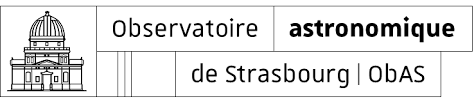
\includegraphics[height=3cm]{Participants/Logos/OAS.png}
\end{center}

The Observatoire Astronomique de Strasbourg (ObAS) is a Joint Research Unit
(UMR7550) of the CNRS and of the Université de Strasbourg. ObAS hosts the 
Centre de Données astronomiques de Strasbourg (Strasbourg astronomical Data 
Centre CDS, http://cds.unistra.fr). Since its creation in 1972, the CDS has 
been providing reference services which are widely used by the world-wide 
astronomical community with more than 1 million queries/day on average in 
2017. The CDS is labelled as a Research Infrastructure in the French national
Research Infrastructure Roadmap. Since 2006 CDS has been the coordinator,
on behalf of the CNRS, of all the projects funded by the European Commission
to support the implementation of European Virtual Observatory. 

% PIC:
% see: http://ec.europa.eu/research/participants/portal/desktop/en/organisations/
%
% See ../proposal.tex, section Members of the Consortium for a
% complete description of what should go there

\subsubsection*{Curriculum vitae}

% Curriculum of the personnel at this institution. This includes
% to-be-hired people for which there is a tentative candidate.

%\input{CVs/First.Last.tex}
%\input{CVs/First.Last.tex}

\input{CVs/Mark.Allen.tex}
\input{CVs/Thomas.Boch.tex}
\input{CVs/Sebastien.Derriere.tex}

\begin{participant}[type=R,PM=12,salary=4200]{Software Engineer}
    We intend to hire a software engineer for 12 months during the project to be be supervised at CDS to work on developments defined in Task \taskref{applications}{astro}. We aim to hire someone in the period of months 12-24. 
\end{participant}

% For other to-be-hired person, please include here something like:
% \begin{participant}[type=res,PM=3,salary=5900]{NN}
%  <a _short_ description of the qualifications of whom you want to hire>
% \end{participant}

\subsubsection*{Publications, products, achievements}

\begin{compactenum}
  \item F. Genova, M. G. Allen, C. Arviset, A. Lawrence, F. Pasian, E. Solano, J. Wambsganss, Euro-VO - Coordination of Virtual Observatory activities in Europe, Astronomy and Computing, 2015, Volume 11, p. 181-189
  \item F. Genova et. al 2017, Building a Disciplinary, World-Wide Data Infrastructure. Data Science Journal, 16: 16, pp. 1-13, DOI: https://doi.org/10.5334/dsj-2017-016
  \item P. Fernique, M. G Allen, T. Boch, A. Oberto, F-X. Pineau, D. Durand, C. Bot, L. Cambresy, S. Derriere, F. Bonnarel, F. Genova, Hierarchical Progressive Surveys - Multi-resolution HEALPix data structures for astronomical images, catalogues and 3-dimensional data cubes.  2015, A \& A, 578, A114 
  \item M. Baumann, T.Boch, New Python developments to access CDS services, Proceedings of The Astronomical Data Analysis Software and Systems conference 2018.
\end{compactenum}

\subsubsection*{Relevant projects or activities}

\begin{compactenum}
  \item ESCAPE (EC funded project, 2019-2023, \#824064, INFRAEOSC-0402018)
  \item ASTERICS (EC funded project, 2015-2019, \#653477, Research and Innovation Action)
  \item AENEAS (EC funded project,  2017-2020, \#731016, Research and Innovation Action)
  \item CoSADIE - Collaborative and Sustainable Astronomical Data Infrastructure for Europe (EC funded project \#312559, 2012-2015, CSA)
  \item RDA Europe - the European plug-in to the Research Data Alliance (RDA) (EC funded project \#632756, 2014-2016, CSA)
\end{compactenum}

\subsubsection*{Significant infrastructure}

CDS is data centre for reference astronomy data. CDS runs physical infrastructure for 1Petabyte. Connected to French national network RENATER. Computing power for X-Match and generation of all-sky survey data. Currently running prototype notebook servers.


\end{sitedescription}
%%% Local Variables:
%%% mode: latex
%%% TeX-master: "../pro%%% End:

\clearpage
\begin{sitedescription}{EP}

\begin{center}

\includegraphics[height=3cm]{Participants/Logos/EP.png}
\end{center}

\'Ecole Polytechnique (l'X), is the leading member of Grandes \'Ecoles in France
for science and technology according to all French rankings last year, ranked
2nd best small university in the world by Times Higher Education in 2018, and
16th best European university by QS World University Rankings in 2018. With
fewer than 3000 Bachelor, Masters, and PhD students enrolled at any time, the
institution has produced 4 Fields Medalists, 4 Nobel prize winners, and 3 French
presidents, ranking it 6th worldwide in terms of number of Nobel prize
recipients. L'X is composed of 22 laboratories supporting research in physics,
engineering, mathematics, biology, and chemistry (among others) and is connected
to several French national research institutions such as CNRS, CEA, and INRIA.
L'X prides itself on promoting multidisciplinary research through collaboration
between its many labs and with external, national and international partners and
a strong connection with industry and start-up.

The Mathematics department at Ecole polytechnique has started a reform of their
various teaching offer based on Jupyter. Many courses from the
Bachelor program, Engineering school, and the Master program have
already begun relying on a strong use of Jupyter notebooks /
JupyterHub\footnote{\url{http://www.cmap.polytechnique.fr/~massot/Personal_web_page_of_Marc_Massot/MAP551}} and this will continue with a strong support of the Dean of
undergraduate studies and of graduate studies. In addition, several software and
research engineers in applied mathematics have been recruited and
participate, together with a system engineer, to this effort in order to help in terms of
building an infrastructure dedicated to Jupyter.
This infrastructure together with support from the head of the Ecole polytechnique,
fosters the dissemination into various other
departments (Physics, Mechanical Engineering, Biology...), where some
Jupyter-based courses are already starting.
A community is emerging, notably through the strong engagement of
students in the computer science club of \'Ecole polytechnique (Binet R\'eseau).

\subsubsection*{Curriculum vitae}
% Curriculum of the personnel at this institution. This includes
% to-be-hired people for which there is a tentative candidate.

\begin{participant}[type=leadPI,PM=8,gender=male]{Loic Gouarin}

  Loic Gouarin is Research Engineer in scientific computing at CMAP (Centre de
  Mathématiques Appliquées) which is a Joint Research Unit
  (UMR7641) of the CNRS and \'Ecole polytechnique. He works on several
  scientific computing open-source projects in different fields such as
  Lattice-Boltzmann methods, Stokes solvers for fluid particles interaction,
  adaptive mesh refinement, ...

  He is also director of the ``GdR Calcul'' where his role is to animate the
  scientific and high performance computing community in France, in particular
  by organising conferences, meetings, and seminars. In this context, he
  organises himself 3 to 4 training and development workshops per year, and
  promotes the use of Python and c++ for teaching and research in France.
  
  For several years, he has been very involved in promoting the Jupyter project
  and its use for teaching and research in the French community. He is one of
  the core developers of xeus-cling and he is working on the possibility of
  easily deploying a JupyterHub or BinderHub on academic clouds. He also
  believes that reproducible research is an essential part of promoting new
  computation codes, new numerical methods, ... introduced in related
  publications and therefore he uses Jupyter as a first approach to achieve this.
  
  \end{participant}
  
  %%% Local Variables:
  %%% mode: latex
  %%% TeX-master: "../proposal"
  %%% End:
  
\begin{participant}[type=R,PM=4,gender=male]{David Delavennat}

    David Delavennat is Research Engineer in scientific infrastructures at CMLS
    (Centre de Mathématiques Laurent Schwartz) which is a Joint Research Unit
    (UMR7640) of the CNRS and \'Ecole polytechnique. He
    works on several french scientific infrastructures projects using
    microservices, virtualization, container and cloud technologies.

    He is coordinator of ARGOS, the Paris-South business network targeted to the
    academic System and Network Administrators. He animates this community,
    organising conferences and meetings He represents ARGOS at RESINFO, the
    french business network of regional SNA business networks. In this context,
    he participate each year to the organization of National Teaching Actions.

    For several years, he has been very involved in promoting the DevOps
    paradigm and Continuous Integration for deploying production infrastructures
    on academic Openstack and Kubernetes environment for the French Mathematical
    community. He is working on simplifying the deployment of a JupyterHub or
    BinderHub onto academic PaaS and Iaas. He also believes that reproducible
    infrastructures is an essential part of reproducible science.

\end{participant}
\input{CVs/Marc.Massot.tex}
\begin{participant}[type=R,PM=2,gender=male]{Laurent Series}

    Laurent Series is Research Engineer in scientific computing at CMAP (Centre 
    de Mathématiques Appliquées) which is a Joint Research Unit
    (UMR7641) of the CNRS and \'Ecole polytechnique. He works on several
    scientific computing open-source projects in different fields like
    finite element method for solid mechanics, multiresolution for 
    reaction-diffusion equations modeling multi-scale reaction wave ...
  
    He was technical responsible of Computing Center (M\'esocentre) of Ecole
    CentraleSup\'elec from 2009 to 2018. In this context, he organises and 
    participates in the user support team (assistance in porting codes, 
    parallelization, vectorisation, optimisation). Since his arrival at \'Ecole 
    Polytechnique, he is involved in the process of creation of a new Computing 
    Center.
    
    For several years, he has been very involved in promoting the Jupyter project
    by writing Jupyter notebooks for course (such as "Dynamical systems for the 
    modeling and simulation of multi-scale reacting media" MAP551) and by promoting, 
    among researchers, its use to share their work. He is also involved with the 
    direction of \'Ecole polytechnique for the project of building an infrastructure 
    for Jupyter at the level of the school, for its use in both research and teaching.
  
\end{participant}

% For other to-be-hired person, please include here something like:
\begin{participant}[type=R,PM=18,salary=5500]{DevOps Engineer}
  We intend to hire a DevOps engineer for 18 months during the project to be supervised at \'Ecole polytechnique to work on developments defined in Tasks \taskref{core}{jh-bh-conv} and \taskref{eosc}{jh-bh-deployment}.
\end{participant}

\begin{participant}[type=R,PM=18,salary=5500]{Software Engineer}
  We intend to hire a DevOps engineer for 18 months during the project to be supervised at \'Ecole polytechnique to work on developments defined in Task \taskref{ecosystem}{teaching-tools}.
\end{participant}

\subsubsection*{Publications, products, achievements}

\begin{compactenum}
\item D. Delavennat, L. Gouarin, G. Philippon, \emph{Deploying JupyterHub with Kubernetes on OpenStack} \newline
\url{https://blog.jupyter.org/how-to-deploy-jupyterhub-with-kubernetes-on-openstack-f8f6120d4b1}
\item JupyterDay at \'Ecole polytechnique in 2018 \newline
\url{http://www.cmap.polytechnique.fr/~massot/Personal_web_page_of_Marc_Massot/JupyterX.html}
\item L. Gouarin, \emph{C++ course using xeus-cling} \newline
\url{https://github.com/gouarin/cours_cpp_moderne}
\item M.Massot, L. Series, \emph{Systèmes dynamiques pour la modélisation et la simulation des "milieux réactifs" multi-échelles} \newline
\url{http://www.cmap.polytechnique.fr/~massot/Personal_web_page_of_Marc_Massot/MAP551}
\end{compactenum}

\subsubsection*{Relevant projects or activities}

\begin{compactenum}
\item Through a previous position at Paris Sud, Loïc Gouarin is a
  participant of OpenDreamKit (GA No. 676541) Open Digital Research
  Environment Toolkit for the Advancement of Mathematics.
\end{compactenum}

\subsubsection*{Significant infrastructure}

\site{EP} has strongly contributed to the deployment of JupyterHub on
\site{UPSUD}'s local OpenStack based cloud infrastructure
\software{Cloud@VD}. \site{EP} invested last year in the purchase of 100 cores for this infrastructure in order to study how to deploy JupyterHub and BinderHub and start to offer to researchers and students this kind of service.
In 2019, \site{EP} will have its own OpenShift cloud infrastructure with 200-300 cores dedicated to teaching with Jupyter.

\end{sitedescription}
%%% Local Variables:
%%% mode: latex
%%% TeX-master: "../proposal"
%%% End:

\clearpage
\begin{sitedescription}{EGI}


The EGI Foundation (also known as Stichting EGI and abbreviated as EGI.eu) 
is a not-for-profit foundation established under the Dutch law to coordinate 
the EGI Federation (abbreviated as EGI), an international collaboration that 
federates the digital capabilities, resources and expertise of national and 
international research communities in Europe and worldwide. 
The main goal is to empower researchers from all disciplines to collaborate 
and to carry out data- and compute-intensive science and innovation. 
The EGI Foundation coordinates areas such as overseeing infrastructure operations, 
user community support, contact with technology providers, strategy and policy 
development, flagship events and dissemination of news and achievements. 
As part of its mandate, the EGI Foundation actively represents the EGI federation 
at European level with policy makers and funding agencies, it provides expert 
advice to shape policies and funding programs and also support the implementation 
of the policy priorities. 
The EGI Foundation holds certifications in both ISO/IEC 9000 “Quality Management” 
and ISO/IEC 20000 “IT Service Management”. 

% PIC:
% see: http://ec.europa.eu/research/participants/portal/desktop/en/organisations/
%
% See ../proposal.tex, section Members of the Consortium for a
% complete description of what should go there

\subsubsection*{Curriculum vitae}
\TODO{AK - rules say "CV or description of the profile of the persons"
  can we name it "Track record" instead of CV?}

% Curriculum of the personnel at this institution. This includes
% to-be-hired people for which there is a tentative candidate.

%\input{CVs/First.Last.tex}
\begin{participant}[type=leadPI,PM=,gender=male]{Gergely Sipos}

    Gergely Sipos works as Technical Outreach Manager for EGI.eu. 
    He coordinates user engagement and supports activities in the EGI community, 
    supporting scientific communities in exploiting EGI services to push scientific 
    boundaries. 

    He holds MSc and PhD in computer science with specialisation in management, 
    from the University of Miskolc (Hungary).

\end{participant}


% For other to-be-hired person, please include here something like:
% \begin{participant}[type=res,PM=3,salary=5900]{NN}
%  <a _short_ description of the qualifications of whom you want to hire>
% \end{participant}

\subsubsection*{Publications, products, achievements}

\begin{compactenum}
\item David, M.; Borges, G.; Pina, J. et al., "Validation of Grid Middleware for the European Grid Infrastructure", (2014) DOI: 10.1007/s10723-014-9301-z 
\item Ferrari, T.; Gaido, L., "Resources and Services of the EGEE Production Infrastructure", Journal of Grid Computing, June 2011, Volume 9, Issue 2, pp 119-133, DOI: 10.1007/s10723-011-9184-1, June 2011. 
\item Matti Heikkurinen, Sandra Cohen, Fotis Karagiannis, Kashif Iqbal, Sergio Andreozzi, Michele Michelotto, "Answering the Cost Assessment Scaling Challenge: Modelling the Annual Cost of European Computing Services for Research", Journal of Grid Computing, May 2014, DOI:10.1007/s10723-014-9302-y 
\item Sy Holsinger, Sergio Andreozzi, "EGI: Implementing service management in a large-scale e-Infrastructure", Proceedings of the IEEE Network Operations and Management Symposium (NOMS) Conference, 2014, Krakow, Poland, DOI: 10.1109/NOMS.2014.6838371
\item Sergio Andreozzi, Sy Holsinger, Damir Marinovic, Steven Newhouse, "EGI: an Open e-Infrastructure Ecosystem for the Digital European Research Area", Proceedings of eChallenges e-2012 Conference, Lisbon, Portugal, ISBN: 978-1-905824-35-91 
\item Ohmann, C.; Canham, S.; Danielyan, E.; Robertshaw, S.; Legr\'e, Y.; Clivio, L. \& Demotes, J., "Cloud computing and clinical trials: report from an ECRIN workshop", Commentary Trials, Springer, December 2015, 16:318, DOI: /10.1186/s13063-015-0835-6 \newline
\item Wallom, D.C.H.; Turilli, M., Drescher, M.; Scardaci, D. \& Newhouse, S., "Federating Infrastructure as a Service Cloud Computing Systems to Creates a Uniform EInfrastructure for Research", IEEE 11th International Conference on e-Science 2015, DOI:10.1109/eScience.2015.51
\item Cloud, Fernandez, E.; Sipos, G.; Scardaci, D.; Wallom, D.C.H. \& Chen, Y., "The user support programme and the training infrastructure of the EGI Federated Cloud", International Conference on High Performance Computing \& Simulation (HPCS) 2015, DOI: 10.1109/HPCSim.2015.7237016 
\item Sergio Andreozzi, Owen Appleton, Sara Coelho, Tiziana Ferrari, Sy Holsinger, Yannick Legr\'e, "Open Science Commons", Jan 2015, http://go.egi.eu/oscwp
\item Kimmo Koski, Kristiina Hormia-Poutanen, Prof. Mike Chatzopoulos, Yannick Legré, Bob Day, "European Open Science Cloud for Research", Oct 2015, https://zenodo.org/record/32915
\end{compactenum}

\subsubsection*{Relevant projects or activities}

\begin{compactenum}
\item EGI-Engage: Engaging the Research Community towards an Open Science Commons
\item EGI-InSPIRE: Integrated Sustainable Pan-European Infrastructure for Researchers in Europe, Project Coordinator, RI-261323
\item AARC (from May 2015)
\item BioMedBridges (Nr 284209)
\item BioVeL (Nr 283359)
\item Civic Epistemologies: Development of a Roadmap for Citizen Researchers in the Digital Culture, RI-632694
\item CloudWATCH: A European cloud observatory supporting cloud policies, standard profiles and services, RI-610994
\item DCH-RP (Nr 312274)
\item e-Fiscal: Financial Study for Sustainable Computing e-Infrastructures, RI-283449
\item EDISON: Creating the Data Science Profession (Nr 675419)
\item ENVRI (Nr 283465)
\item ENVRIplus (Nr 654182)
\item ER-Flow (Nr 312579)
\item eScienceTalk: Supporting grid and high performance computing reporting across Europe, Project Coordinator, RI-260733
\item FedSM: Implementing Service Management in Federated e-Infrastructures, RI-312851
\item Helix Nebula Science Cloud Project, the (from January 2016)
\item HelixNebula: Big science teams up with big business, RI-312301
\item INDIGO-DataCloud (from May 2015)
\end{compactenum}

\subsubsection*{Significant infrastructure}

EGI Infrastructure: The EGI Foundation coordinates the delivery of the EGI Infrastructure that brings together more than 300 data centres worldwide and also includes the largest community cloud federation in Europe with 21 cloud providers across 12 European countries offering IaaS cloud and storage services. The Infrastructure includes a Jupyter Hub that is open for researchers on the scalable EGI IaaS cloud.

\end{sitedescription}
%%% Local Variables:
%%% mode: latex
%%% TeX-master: "../proposal"
%%% End:

\clearpage
\begin{sitedescription}{XFEL}
  \label{sitedescription:euxfel}

% PIC:
% see: http://ec.europa.eu/research/participants/portal/desktop/en/orga

% See ../proposal.tex, section Members of the Consortium for a
% complete description of what should go there

  European X-Ray Free-Electron Laser Facility GmbH is a limited
  liability company under German law. At present, 12 countries are
  participating in the project: Denmark, France, Germany, Hungary,
  Italy, Poland, Russia, Slovakia, Spain, Sweden, Switzerland, and the
  United Kingdom.  The company is in charge of the operation and
  construction of the European XFEL, a 3.4 km long X-ray free-electron
  laser facility extending from Hamburg to the neighbouring town of
  Schenefeld in the German federal state of Schleswig-Holstein. Civil
  construction started in early 2009, and the user operation in
  September 2017. With its repetition rate of 27,000 pulses per second
  and a peak brilliance a billion times higher than that of the best
  synchrotron X-ray radiation sources, the European XFEL will allow
  the investigation of still open scientific problems in a variety of
  disciplines (physics, structural biology, chemistry, planetary
  science, study of matter under extreme conditions and many others).

  European XFEL has a data policy in place \cite{datapolicy-euxfel}
  which opens up facility data for open access after an embargo period
  of 3 years.
\subsubsection*{Curriculum vitae}

% Curriculum of the personnel at this institution
%
\input{CVs/Hans.Fangohr.tex}
\input{CVs/Sandor.Brockhauser.tex}
\begin{participant}[type=PI,PM=1,gender=male]{Krzysztof Wrona}
  % type is one of:
  % - leadPI: leader of the participating institution
  % - PI: Principal Investigator
  % - R: researcher?
  % Who is the coordinator is specified elsewhere

  % PM=YYY:
  % A fair evaluation of the number of months you will be
  % spending on this specific project along the four years.
  % Typical numbers:
  % - full time hired personnel: 48 months
  % - lead PI or proposal coordinator: 8-12 months
  % - PI: 4-5 months
  % - participant: 2-6 months

  % salary=ZZZ:
  % Approximate monthly gross salary (in term of total cost for the
  % employer). This is optional. If you are uncomfortable having this
  % information in a public file, you can alternatively send the
  % information to Eugenia Shadlova, or to your institution
  % leader/manager if he is willing to fill in himself the budget
  % forms on the eu portal.

  % The above information is used to fill in various tables in the
  % proposal file, and to evaluate the cost of the project for the
  % institutions.

  % You may remove all those comments.

  % About half a page of free text; for whatever it's worth, you may see
  % Nicolas.Thiery.tex for an example.



  \medskip Krzysztof Wrona has a background in computer physics. As
  the group leader of IT and Data Management at European XFEL, he is
  in charge of the management of scientific data in the frame of the
  user program of the European XFEL facility. He has more than 15
  years of experience in data storage, processing, and in general IT
  issues.
\end{participant}

%%% Local Variables:
%%% mode: latex
%%% TeX-master: "../proposal"
%%% End:

\input{CVs/Thomas.Kluyver.tex}
%


\begin{participant}[PM=68, type=R]{Research Engineer x2}

We will hire two postdoctoral-level research software engineers (for 68 person
months in total) to carry out the required work for this projet at
European XFEL. They will work under supervision of Hans Fangohr, with
support from Sandor Brockhauser and Krzysztof Wrona for particular
aspects. The employees will either have a scientific background and
significant software engineering expertise, or an education in
computer science and an aptitude to work with scientists on
computational science and data science problems.
\end{participant}

\subsubsection*{Publications, products, achievements}

\begin{compactenum}
\item H.Fangohr, Python for Computational Science and Engineering
  (2018) DOI: 10.5281/zenodo.1411868 \newline
  https://github.com/fangohr/introduction-to-python-for-computational-science-and-engineering
\item H.Fangohr et al., “Data Analysis support in Karabo at European
  XFEL”, Proceedings of International Conference on Accelerator and
  Large Experimental Physics Control Systems 2017, ISBN 978-3-95450-
  193-9, Data Analytics, Barcelona, Spain, TUCPA01 (2017) DOI: 10.18429/JACoW-ICALEPCS2017-TUCPA01
\item H.Fangohr.
\emph{A Comparison of \software{C}, \Matlab and \Python as Teaching Languages in Engineering}
Lecture Notes on Computational Science \textbf{3039}, 1210-1217 (2004)
\item T. Kluyver, B. Ragan-Kelley, F. Perez, B. Granger, M. Bussonier, J. Frederic, K. Kelley, J. Hamrick, J. Grout, S. Corlay et al. Jupyter
\emph{Notebooks: a publishing format for reproducible computational workflows} In 20th International Conference on Electronic Publishing. IOS Press, 2016.
\end{compactenum}

\subsubsection*{Relevant projects or activities}

\begin{compactenum}
\item OpenDreamKit (GA No. 676541) Open Digital Research Environment
  Toolkit for the Advancement of Mathematics, participant
\item EOSCpilot (GA No. 739563) The European Open Science Cloud for
  Research Pilot Project, participant
\item PaNOSC (GA No. 823852) Photon and Neutron Open Science Cloud,
  participant
\item CALIPSOplus (GA No. 730872) Convenient Access to Light Sources
  Open to Innovation, Science and to the World, participant
\item ATTRACT (GA No. 777222) breAkThrough innovaTion pRogrAmme for a
  pan-European Detection and Imaging eCosysTem, participant

\end{compactenum}




\end{sitedescription}



%KEY-MORE-TODOS



%%% Local Variables:
%%% mode: latex
%%% TeX-master: "../proposal"
%%% End:

%  LocalWords:  sitedescription Programme organisations programmes Centres subsubsection
%  LocalWords:  micromagnetic Nmag Fischbacher Franchin Bordignon Fangohr emph textbf
%  LocalWords:  Multiphysics summarised Iridis TFlops Modelling

\clearpage
\begin{sitedescription}{INSERM}

Inserm, the French National Institute of Health \& Medical Research is the only
public sector research institution in France exclusively dedicated to human
health. Under the dual aegis of the Ministries of Health and Research, Inserm
has a budget of 900 M euros and employs 15,000 scientists, engineers and
technicians all with one shared objective, namely to promote health - by
advancing knowledge about living organisms and their diseases, developing
innovative treatment modalities and conducting research on public health.

Inserm is represented within the BOSSEE consortium through the Cancer Research
Centre of Toulouse (CRCT) and Inserm’s Computing Department (D\'epartement du
Système D’Information, DSI).

CRCT gathers academic, scientific, medical, clinical, technological and
pharmaceutical research on cancer on a 220-hectares site next to Toulouse,
France. Its missions are to improve fundamental knowledge on all aspects of
cancer biology and to provide patients with rapid access to innovative and
individualized treatments. On these premises, CRCT comprises 21 teams
affiliated to Inserm, the University of Toulouse and the CNRS (National Centre
for Scientific Research). Team 15 of CRCT led by M. Bardi\`es aggregates
Medical Physics resources available in Toulouse around a common research theme:
the optimization of radiotherapy through the development of innovative
dosimetric approaches at various scales (cell, tissue, patient).

Inserm's IT department (DSI) defines and coordinates IT and information systems
aspects across the whole institution. It designs and operates Inserm's
information system to support research activities of the institute, and
provides counselling and support to research units on information technologies.
It also plays a strong role in coordinating IT security and risk management
policies for the French health science community.

% PIC:
% see: http://ec.europa.eu/research/participants/portal/desktop/en/organisations/
%
% See ../proposal.tex, section Members of the Consortium for a
% complete description of what should go there

\subsubsection*{Curriculum vitae}
% Curriculum of the personnel at this institution. This includes
% to-be-hired people for which there is a tentative candidate.
\begin{participant}[type=leadPI,PM=3,gender=male]{Manuel Bardi\`es}
  % type is one of:
  % - leadPI: leader of the participating institution
  % - PI: Principal Investigator
  % - R: researcher?
  % Who is the coordinator is specified elsewhere

  % PM=YYY:
  % A fair evaluation of the number of months you will be
  % spending on this specific project along the four years.
  % Typical numbers:
  % - full time hired personnel: 48 months
  % - lead PI or proposal coordinator: 8-12 months
  % - PI: 4-5 months
  % - participant: 2-6 months

  % salary=ZZZ:
  % Approximate monthly gross salary (in term of total cost for the
  % employer). This is optional. If you are uncomfortable having this
  % information in a public file, you can alternatively send the
  % information to Eugenia Shadlova, or to your institution
  % leader/manager if he is willing to fill in himself the budget
  % forms on the eu portal.

  % The above information is used to fill in various tables in the
  % proposal file, and to evaluate the cost of the project for the
  % institutions.

  % You may remove all those comments.

  % About half a page of free text; for whatever it's worth, you may see
  % Nicolas.Thiery.tex for an example.

  Manuel Bardi\`es, PhD, obtained his doctorate on radiopharmaceutical
  dosimetry from Paul Sabatier University (Toulouse III) in 1991. He has been
  developing his research in radiopharmaceutical dosimetry within INSERM
  (National Institute of Health and Medical Research), since 1992, in Nantes
  then in Toulouse (2011) within the Cancer Research Centre of Toulouse (CRCT).
  He is the responsible of CRCT Team 15 entitled "Multi- resolution dosimetry
  for radiotherapy optimization".
  
  Dr. Bardi\`es has been appointed to several international positions. He was
  one of the founders of the EANM Dosimetry Committee (member from 2001 to
  2013, chair 2009-2011). He also chaired of EFOMP Science Committee
  (2014-2016).
  
  Dr. Bardi\`es is also involved in education and is currently member of the
  Board of the European School for Medical Physics Expert (ESMPE) and member of
  the European School of Multimodality Imaging and Therapy (ESMIT).
  
  The team led by Manuel Bardi\`es in Toulouse (CRCT Team 15) is primarily
  involved in radiopharmaceutical dosimetry, at various scales (cell, tissue,
  organs). This requires the ability to assess radiopharmaceutical
  pharmacokinetics in vivo, through quantitative SPECT or PET small-animal
  imaging. An important part of research activity is related to Monte Carlo
  modelling of radiation transport through biological structures of interest,
  in order to give account of energy deposition within tumour targets - or
  critical non-tumour tissues/organs. The objective is to improve molecular
  radiotherapy by allowing patient-specific treatments, as an important
  application of personalized medicine.

\end{participant}

%%% Local Variables:
%%% mode: latex
%%% TeX-master: "../proposal"
%%% End:

\input{CVs/Maxime.Chauvin.tex}
\begin{participant}[type=PI,PM=6,gender=female]{Isabelle Perseil}
  % type is one of:
  % - leadPI: leader of the participating institution
  % - PI: Principal Investigator
  % - R: researcher?
  % Who is the coordinator is specified elsewhere

  % PM=YYY:
  % A fair evaluation of the number of months you will be
  % spending on this specific project along the four years.
  % Typical numbers:
  % - full time hired personnel: 48 months
  % - lead PI or proposal coordinator: 8-12 months
  % - PI: 4-5 months
  % - participant: 2-6 months

  % salary=ZZZ:
  % Approximate monthly gross salary (in term of total cost for the
  % employer). This is optional. If you are uncomfortable having this
  % information in a public file, you can alternatively send the
  % information to Eugenia Shadlova, or to your institution
  % leader/manager if he is willing to fill in himself the budget
  % forms on the eu portal.

  % The above information is used to fill in various tables in the
  % proposal file, and to evaluate the cost of the project for the
  % institutions.

  % You may remove all those comments.

  % About half a page of free text; for whatever it's worth, you may see
  % Nicolas.Thiery.tex for an example.

  Isabelle Perseil, PhD, is the Head of the Computational Science Coordination
  and e-infrastructures of Inserm. Dr. Perseil manages a group of 3 experts
  which provides the best practices in software engineering, Data Management,
  Big data, deep learning, HPC, Grids, Cloud Computing, parallel computing to
  300 research units (1200 research teams).
  
  The Computational Science Coordination is working with 13 regional
  administrations and 23 regional Mesocenters to pool the computational
  resources (grids and HPC) and train more than 1000 engineers and researchers
  to HPC (OpenMP, MPI and now ORWL) and Big data (MapReduce, Hadoop, Spark,
  Flink, Storm).

\end{participant}

%%% Local Variables:
%%% mode: latex
%%% TeX-master: "../proposal"
%%% End:

\input{CVs/Gilles.Mathieu.tex}

% For other to-be-hired person, please include here something like:
% \begin{participant}[type=res,PM=3,salary=5900]{NN}
%  <a _short_ description of the qualifications of whom you want to hire>
% \end{participant}

\subsubsection*{Publications, products, achievements}
\begin{compactenum}
\item A. Albeyatti et al. “Towards a European health research and innovation
  cloud (HRIC)”. In: 2019 accepted in Genome Medicine.
\item M. Chauvin et al. “OpenDose: Generating reference data for Nuclear
  Medicine dosimetry”. In: European Journal of Nuclear Medicine and Molecular
  Imaging 44.S2 (Sept. 2017), pp. 119--956. DOI: 10.1007/s00259-017-3822-1.
\item D. Salas et al. “Resource-Centered Distributed Processing of Large
  Histopathology Images”. In: 2016 IEEE Intl Conference on Computational
  Science and Engineering (CSE) and IEEE Intl Conference on Embedded and
  Ubiquitous Computing (EUC) and 15th Intl Symposium on Distributed Computing
  and Applications for Business Engineering (DCABES). Aug. 2016, pp. 367--370.
  DOI: 10.1109/CSE-EUC-DCABES.2016.210.
\item S. Marcatili et al. “Model-based versus specific dosimetry in diagnostic
  context: Comparison of three dosimetric approaches”. In: Medical Physics 42.3
  (2015), pp. 1288--1296. DOI: 10.1118/1.4907957.
\item D. Sarrut et al. “A review of the use and potential of the GATE Monte
  Carlo simulation code for radiation therapy and dosimetry applications”. In:
  Medical Physics 41.6 Part1 (2014), p. 064301. DOI: 10.1118/1.4871617.
\item I. Perseil et al. “An Efficient Modeling and Execution Framework for
  Complex Systems Development”. In: 2011 16th IEEE International Conference on
  Engineering of Complex Computer Systems. Apr. 2011, pp. 317--331. DOI:
  10.1109/ICECCS.2011.38.
\item  A. Divoli et al. “Effect of Patient Morphology on Dosimetric
  Calculations for Internal Irradiation as Assessed by Comparisons of Monte
  Carlo Versus Conventional Methodologies”. In: Journal of Nuclear Medicine
  50.2 (2009), pp. 316--323. DOI: 10.2967/jnumed.108.056705.
\item I. Perseil and L. Pautet. “Foundations of a new software engineering
  method for real-time systems”. In: Innovations in Systems and Software
  Engineering 4.3 (Oct. 2008), pp. 195--202. ISSN: 1614-5054. DOI:
  10.1007/s11334-008-0067-y
\end{compactenum}

\subsubsection*{Relevant projects or activities}
Inserm is the leading academic biomedical research institution in Europe with
more than 13,000 publications a year; and second in the world (behind the
American National Institutes of Health).

Inserm has 24 international cooperation agreements, 33 associated European
laboratories (AELs) and associated international laboratories (AILs), and 183
Horizon 2020 contracts since 2014 - of which 45 were signed in 2017. 67 ERC
winners have been hosted at Inserm since 2012, 13 of whom in 2017.  Inserm is
involved in many ESFRIs:
\begin{compactenum}
\item ERINHA2 (H2020)
\item ERINHA (FP7)
\item ADOPT BBMRI-ERIC (H2020)
\item BioMedBridges (FP7)
\item MRTdosimetry EMPIR (H2020)
\item MetroMRT (REG)
\end{compactenum}
Inserm is also one of the funding partners of the French NGI, integrated within
EGI.

\subsubsection*{Significant infrastructure}
Inserm has more than 350 research units spread across France and
internationally. These are supported by 13 Regional Commissions for local
oversight. Scientific activities are organized around 9 “Inserm Thematic
Institutes”, corresponding to the main fields of biomedical and health
research.

\end{sitedescription}
%%% Local Variables:
%%% mode: latex
%%% TeX-master: "../proposal"
%%% End:

\clearpage
\begin{sitedescription}{QS}

\begin{center}

\includegraphics[height=3cm]{Participants/Logos/QuantStack.png}
\end{center}

\par QuantStack was founded in 2016 by a team of developers and maintainers of key packages of the open-source scientific computing stack. QuantStack provides support and custom development services in the Jupyter and Scientific Python ecosystems. Clients and partners of QuantStack range from financial software companies to robotics startups and public research institutions. The team comprises several core developers of Jupyter subprojects and authors of popular scientific computing and visualization software used in both academic and industrial contexts.

\par Beyond Project Jupyter, projects developed at QuantStack include data visualization packages for Jupyter such as bqplot, ipyvolume, ipyleaflet, and ipysheet, as well as Jupyter language kernels such as xeus-cling and xeus-python, and JupyterLab extensions like te draw.io and sidecar. QuantStack is also behind the development of the xtensor framework, a high-level array computing library and C++ dataframe.

\subsubsection*{Curriculum vitae of the investigators}

\input{CVs/Sylvain.Corlay.tex}
\input{CVs/Johan.Mabille.tex}
\input{CVs/Martin.Renou.tex}
\input{CVs/Wolf.Vollprecht.tex}

% For other to-be-hired person, please include here something like:
\begin{participant}[type=R,PM=41,salary=7000]{Software Engineer} %% Salary: standard SME cost
  We will hire a software engineer with experience working in large open-source
  projects. They will benefit from the mentoring of the other Jupyter contributors
  of the QuantStack team.
\end{participant}

\subsubsection*{Publications, products, achievements}

\begin{compactenum}

\item QuantStack developers participate in the continuous development of \emph{Project Jupyter}. The team is especially active in the area of interactive widgets, as well as JupyterLab and the Jupyter Server.

\item QuantStack is the main driving force behind the \emph{xtensor} project, a C++ tensor expression system for high-performance computing. Xtensor comes along with language bindings for Python, R, and Julia, as well as interfaces to BLAS, FFTW, and means to input and output a large number of standard file formats.

\item QuantStack also develops the \emph{xeus} project, a framework for creating Jupyter language kernels. Xeus is used as a foundation for the C++ Jupyter kernel "xeus-cling", built upon the Cling C++ interpreter from CERN. Xeus was also adopted in Kitware's \emph{Slicer} medical imaging software for its Jupyter integration.

\item The QuantStack team includes the authors and maintainers of some of the most popular Jupyter interactive widgets packages, including \emph{bqplot}, a 2-D interactive plotting system, \emph{ipyvolume}, a 3-D volume rendering package, \emph{ipyleaflet}, a maps visualization toolkit.

\item QuantStack contributes extensively to the \emph{conda-forge} project, a community-maintained collection of packages for scientific computing. Nearly a hundred "recipes" for conda-forge are maintained by QuantStack.

\item QuantStack developers are also behind the \emph{vaex} data decimation engine for interactive visualization of large datasets.

\end{compactenum}

\subsubsection*{Relevant projects or activities}

\par Beyond open-source scientific computing development, QuantStack promotes scientific open source software development through the organization of events and by volunteering in non-profit organizations promoting the ecosystem.

\begin{compactenum}

\item QuantStack team members co-organize the regular \emph{PyData Paris Meetup}, a free event series taking place every two to three months. After a year, the group counts over two thousand members in Paris.

\item We also support the \emph{NumFOCUS Fondation} as volunteers as a member of the team is a member of the board of directors of the foundation.

\end{compactenum}

% \subsubsection*{Significant infrastructure}

\end{sitedescription}

%%% Local Variables:
%%% mode: latex
%%% TeX-master: "../proposal"
%%% End:

\clearpage
\begin{sitedescription}{UIO} \label{desc:UIO}

The University of Oslo (UiO) is Norway's oldest institution for research and higher education, with 28,000 students and 6,000 employees. UiO has 8 faculties, 2 museums and several centres. In addition, UiO has 10 Norwegian Centres of Excellence,  is ranked as the world's 62nd university, and has had 5 Nobel prize laureates. UiO aims to become an international hub for the research-based integration of computing into science education and has financed a university-wide hosting service for Jupyter notebooks through JupyterHub  to introduce a computational aspect to all curriculum programs in all science disciplines from bachelor to postdoctoral studies.

The University of Oslo is a Silver Partner to \href{https://carpentries.org}{The Carpentries}, an international successful community driven project with Instructors, Trainers, Maintainers, helpers, and supporters who share a mission to teach foundational computational and data science skills to researchers.

The Department of Geosciences of the Faculty of Mathematics and Natural Sciences is the broadest geoscience research-based teaching environment in Norway, and covers a wide range of disciplines from deep mantle processes to atmospheric sciences. It is organised in five sections and an administrative unit and supports two main strategic research initiatives:

- Land-Atmosphere Interactions in Cold Environments (\href{https://www.mn.uio.no/geo/english/research/groups/latice/}{LATICE})

- Interface Dynamics in Geophysical Flows (\href{https://www.mn.uio.no/geo/english/research/groups/earthflows/}{EarthFlows})


 The geosciences department has several large research projects financed by \href{https://www.forskningsradet.no/en/Home_page/1177315753906}{The Research Council of Norway}, EU and Norwegian companies.

 The University of Oslo aims to manage research data according to international standards, such as the \href{https://www.uio.no/for-ansatte/arbeidsstotte/fa/forskningsdata/fair-data/index.html}{FAIR principles}\footnote{Findable, Accessible, Interoperable and Reusable}, and thereby support the development of a global research community in which research data is widely shared.
 Since November 2017, UiO’s policy follows the "open as standard" principle in respect of access to research data \cite{datapolicy-uio}.

\subsubsection*{Curriculum vitae}

% Curriculum of the personnel at this institution. This includes
% to-be-hired people for which there is a tentative candidate.

\begin{participant}[type=R,PM=24,gender=female]{Anne Fouilloux}
  % type is one of:
  % - leadPI: leader of the participating institution
  % - PI: Principal Investigator
  % - R: researcher?
  % Who is the coordinator is specified elsewhere

  % PM=YYY:
  % A fair evaluation of the number of months you will be
  % spending on this specific project along the four years.
  % Typical numbers:
  % - full time hired personnel: 48 months
  % - lead PI or proposal coordinator: 8-12 months
  % - PI: 4-5 months
  % - participant: 2-6 months

  % salary=ZZZ:
  % Approximate monthly gross salary (in term of total cost for the
  % employer). This is optional. If you are uncomfortable having this
  % information in a public file, you can alternatively send the
  % information to Eugenia Shadlova, or to your institution
  % leader/manager if he is willing to fill in himself the budget
  % forms on the eu portal.

  % The above information is used to fill in various tables in the
  % proposal file, and to evaluate the cost of the project for the
  % institutions.

  % You may remove all those comments.

  % About half a page of free text; for whatever it's worth, you may see
  % Nicolas.Thiery.tex for an example.

  \medskip PhD, is a highly experienced Research Software Engineer dedicated to supporting
  researchers towards the adoption of Open Science best practices.

  With a solid background in Computer Sciences, she worked in various application fields, including environmental sciences, Intelligent Transport Systems, High-Performance computing, bio-informatics, meteorology and Geosciences.

  She is currently working in the IT group of the department of Geosciences at the University of Oslo\footnote{\url{https://www.mn.uio.no/geo/english}} and for the Nordic e-Infrastructure Collaboration (NeIC\footnote{\url{https://neic.no}}) where she is involved on the NICEST\footnote{Nordic Collaboration on e-Infrastructures for Earth System Modeling, \url{https://neic.no/nicest/}} and CodeRefinery\footnote{Training and e-Infrastructure for Research Software Development, \url{https://coderefinery.org/}} projects. 

   Since 2015, Anne Fouilloux has been very active with The Carpentries\footnote{\url{https://carpentries.org}}, a diverse and global community of volunteers and she teaches foundational coding and data science skills to students and young researchers. She is a certified Carpentries instructor\footnote{\url{https://carpentries.org/instructors/}}, instructor trainer\footnote{\url{https://carpentries.org/trainers/}} and maintainer\footnote{\url{https://carpentries.org/maintainers/}}. She has volunteered to help build CarpentryCon 2020\footnote{\url{http://www.carpentrycon.org/}} a biannual conference for members of the global Carpentries community and people with similar interests. 

  She is a member of the core team of the Carpentries@UiO\footnote{\url{https://www.uio.no/english/for-employees/support/research/research-data/training/carpentry/}} and is leading the studyGroup@UiO\footnote{\url{https://uio-carpentry.github.io/studyGroup/}} where students and researchers at the University of Oslo are committed to sharing skills, experiences, and ideas around open science, open source, code, and community in research.
\end{participant}

%%% Local Variables:
%%% mode: latex
%%% TeX-master: "../proposal"
%%% End:


%\input{CVs/First.Last.tex}
%\input{CVs/First.Last.tex}
%\input{CVs/First.Last.tex}

% For other to-be-hired person, please include here something like:
% \begin{participant}[type=res,PM=3,salary=5900]{NN}
%  <a _short_ description of the qualifications of whom you want to hire>
% \end{participant}

\subsubsection*{Publications, products, achievements}

\begin{compactenum}
\item \href{https://annefou.github.io/jupyter_publish/}{Publication ready scientific reports and presentations with Jupyter notebooks}, Anne Fouilloux, Research Bazaar 2019, \href{https://zenodo.org/badge/latestdoi/163517733}{DOI 10.5281/zenodo.2548936}

\item \href{https://annefou.github.io/jupyter_dashboards/}{Reproducible Research with Interactive Jupyter Dashboards}, 2018, Ana Costa Conrado, Gladys Nalvarte, Benjamin Ragan-Kelley and Anne Fouilloux, Research Bazaar 2018, \href{https://zenodo.org/badge/latestdoi/114125668}{DOI 10.5281/zenodo.1168721}

\item \href{https://annefou.github.io/metos_python/}{Working with Spatio-temporal data in Python}, 2017, Anne Fouilloux, \href{https://zenodo.org/badge/latestdoi/96184802}{DOI 10.5281/zenodo.1165281}
\end{compactenum}

\subsubsection*{Relevant projects or activities}

\begin{compactenum}
\item \href{https://coderefinery.org}{CodeRefinery} \label{desc:coderefinery} (2016-2021): 


The goal of this project is to provide students and researchers with infrastructure and training in the necessary tools and techniques to create sustainable, modular, reusable, and reproducible software.
This is a project within the Nordic e-Infrastructure Collaboration (\href{https://neic.no}{NeIC}), an organisational unit under \href{https://www.nordforsk.org/en}{NordForsk}.
NeIC is a Platinium Partner to \href{https://carpentries.org}{The Carpentries}.

The result of this project is a set of software development e-infrastructure solutions, coupled with necessary technical expertise and extensive training and on-boarding activities, training material and best practices guides which together form a Nordic platform for research groups and institutes to develop a better collaboration on software and thereby to catalyze reproducible research and collaboration.
\newline
CodeRefinery training material is licensed under \href{https://creativecommons.org/licenses/by-sa/4.0/}{CC BY-SA 4.0} and code examples are \href{https://opensource.org/}{OSI}-approved \href{https://opensource.org/licenses/mit-license.html}{MIT license}.

The University of Olso is a CodeRefinery partner and will ensure the complementarity of the two projects thus avoiding potential fragmentation. \TheProject will benefit from all this experience as well as the estbalished network in the Nordic Countries and beyond to fully realize the potential of \TheProject EOSC services. 
\newline


\item Nordic Collaboration on e-Infrastructures for Earth System Modeling (\href{https://neic.no/nicest}{NICEST}, 2017-2019) \label{desc:nicest}:

This project aims at networking, intensifying existing collaboration, and facilitating 
joint work on very specific topics helping, for example, building up knowledge and
competency, and harmonising certain procedures concerning e-Infrastructure topics.

\item \href{https://uiohive.github.io/Hive/}{UiOHive} (2018-2019) \label{desc:uiohive}: 

UiOHive provides a vital and novel competence at the Union of Internet of Things (IoT), Microcontroller / Hardware development, Artificial Intelligence (AI) and Machine Learning, and Data Science to enhance and strengthen collaboration between domains at the application of the aforementioned technologies. and the disciplines with competence to further develop technologies.
The purpose of GEOHive is to establish a central knowledge hub, centered around individuals interested in utilizing IoT technologies, applying Artificial Intelligence and Machine Learning to data challenges, and sharing knowledge across relevant interdisciplinary domains.

\item \href{https://www.mn.uio.no/geo/english/research/groups/latice/}{LATICE} (Land-ATmosphere Interactions in Cold Environments, 2015-2022): 
LATICE aims to advance the knowledge base concerning land atmosphere interactions and their role in controlling climate variability and climate change at high northern latitudes.

\item \href{https://www.mn.uio.no/geo/english/research/groups/earthflows/}{EarthFlows} (Interface Dynamics in Geophysical Flows, 2015-2022): 
The dynamics of interface processes during flows on Earth, including the geosphere, the hydrosphere, the cryosphere, and the atmosphere, including the behavior of the complex interfaces separating ‘Fluid Earth’ from ‘Solid Earth’.

The goal for the EarthFlows project is to provide fundamentally new understanding of the dynamics of fluid-solid interfaces for a number of important geophysical systems.

\end{compactenum}

\subsubsection*{Significant infrastructure}

\begin{compactenum}

\item \href{http://www.uh-iaas.no/}{Infrastructure as a Service}: the University of Oslo is part of the Norwegian Cloud Infrastructure for Research and Education and provide researchers with compute and storage medium-size resources. These include multi-GPUs clusters for big data analysis. The department of Geosciences is heavily relying on this services both for teaching and research work.

\item \href{https://sigma2.no}{UNINETT Sigma-2}: UNINETT Sigma2 manages the national infrastructure for computational science in Norway and offers services in High Performance Computing (HPC) and Data Storage and data analysis (Research Platform as a Cloud Service). The services are organized into infrastructural activities, financed by the Research Council of Norway and the Sigma2 consortium partners, which are the universities in Oslo, Bergen, Trondheim and Tromsø.

Services are freely available to individuals and groups involved in  research and education at Norwegian universities and colleges, and other organizations and project funded with public money. Cost efficient development, procurement, coordination and operation of the national e-infrastructure for research and education is the main focus for Sigma2.

The Department of Geosciences (University of Oslo) has been granted access to over 2 petabytes and several millions of CPU hours on the Norwegian High-Performance computers.
\end{compactenum}

\end{sitedescription}
%%% Local Variables:
%%% mode: latex
%%% TeX-master: "../proposal"
%%% End:

\clearpage
\begin{sitedescription}{UPSUD} \label{desc:ParisSud}

Université Paris-Sud is among the 40 top universities worldwide in the
2013 Shanghai ranking, and is one of the top two French research
universities. With about 27000 students, 1800 permanent faculty
and 1300 permanent research scientists from national research
organisations (CNRS, Inserm, INRA, Inria), it is the largest campus in
France. Since 2006, scientists from the University were awarded two
Fields medals, one Nobel Prize and a number of other national and international prizes
(European Inventor Award 2013, Wolf Prize 2010, Holweck Prize 2009,
Japan prize 2007).  Université Paris-Sud offers a
wide range of qualifications, from the exact sciences to life and health
sciences (including medical practice), legal sciences and economics. 
Research at Université Paris-Sud is an essential part of academic understanding 
and includes research activities with high commercial potential. 
Research contracts and partnership with companies make
Université Paris-Sud a key actor and a major player in French
research.  The University is located partly on the Plateau de Saclay,
the largest cluster of public and private R\&D institutions in France
(with ca. 16000 research staff), and is one of the core members of 
University Paris-Saclay – a world-class university and a
world-renowned research and innovation hub.

In the context of this project, Université Paris-Sud is the
home of one of the largest group of \Sage developers worldwide.
It is a member of the Open Source Thematic Group of the Systematic
Paris Region Systems and ICT Cluster. 
The University also hosts a major research group in Human-Centered Computing
and manages the Digiscope network of high-end visualisation platforms,
which will provide critical assets to the project.

\subsubsection*{Curriculum vitae of the investigators}

\begin{participant}[type=PI,PM=2,gender=male]{Michel Beaudouin-Lafon}

Michel Beaudouin-Lafon (PhD, Université Paris-Sud) is a Professor of Computer Science, classe exceptionnelle, 
at Université Paris-Sud and a senior fellow of Institut Universitaire de France. 
His research interests include fundamental aspects of interaction, novel interaction techniques, 
computer-supported cooperative work and engineering of interactive systems. 
He has published over 180 papers and is a member of the ACM SIGCHI Academy. 
He is the laureate of an ERC Advanced Grant exploring instrumental interaction and information substrates. 
Michel was director of LRI, the laboratory for computer science joint between Université Paris-Sud and CNRS. 
He now heads the Human-Centered Computing lab at LRI and chairs the Computer Science department at Université Paris-Saclay. 
He was Technical Program Co-chair for CHI 2013 (3500 participants), sits on the editorial boards of ACM Books and ACM TOCHI, 
and has served on many ACM committees. He received the ACM SIGCHI Lifetime Service Award in 2015.

\end{participant}

%%% Local Variables:
%%% mode: latex
%%% TeX-master: "../proposal"
%%% End:

\begin{participant}[type=PI,PM=2,gender=female]{Viviane Pons}
  Maître de Conférences at the Laboratoire de Recherche en Informatique, Viviane Pons is a
  young researcher in Algebraic Combinatorics. She defended her thesis in 2013 and has 4
  papers in international journals and 5 communications in international
  conferences, including a talk at PyCon US 2015. 
  She also is in the editorial board of the Journal of Open Source Software.
  Before starting her research career,
  she worked for two years in industry as a Java and web developer.

  She discovered \Sage during her first \Sage Days in 2010 and has since been an active user
  and contributor with 10 (co)authored tickets improving the support of combinatorial
  objects in \Sage. She is heavily involved in the promotion of \Sage, participating in
  \Sage Days and running \Sage introduction tutorials or \Sage presentations at various
  conferences. She is also one of the main developers of the project \software{FindStat}
  dedicated to databases in combinatorics.

  Viviane is leading the very successful Community Building and
  Dissemination work package of the European Research Infrastructures
  project OpenDreamKit (2015-2019), in which 66 events (development
  workshops, training sessions, ...) were organized or coorganized,
  with more than a thousand trainees. Viviane herself organized or
  coorganized several of them, including two week-long workshops
  dedicated to women.
\end{participant}
%%% Local Variables:
%%% mode: latex
%%% TeX-master: "../proposal"
%%% End:

\begin{participant}[type=leadPI,PM=5,gender=male]{Nicolas M. Thiéry}
  Professor at the Laboratoire de Recherche en Informatique, Nicolas
  M. Thiéry is a senior researcher in Algebraic Combinatorics with 18
  papers published in international journals. Among other things, he
  is a member of the permanent committee of FPSAC, the main
  international conference of the domain, a founding member of the
  upcoming Numfocus Europe non-profit, and a member of Work group on
  Free and Open Source software for the ``Open Science Committee'' of
  the French Ministry for Research.
  He has collaborators
  in the US and Canada where he cumulatively spent more than three
  years (Colorado School of Mines, UC Davis, Providence, Montréal),
  and in India. He also
  co-organised fourteen international workshops, in particular \Sage Days, and the semester
  long program on ``Automorphic Forms, Combinatorial Representation Theory and Multiple
  Dirichlet Series'' hosted in Providence (RI, USA) by the Institute for Computational and
  Experimental Research in Mathematics.

  Algebraic combinatorics is a field at the frontier between mathematics and computer
  science, with heavy needs for computer exploration. Pioneer in community-developed open
  source software for research in this field, Thiéry founded in 2000 the \SageCombinat
  software project (incarnated as \MuPADCombinat until 2008); with 50 researchers
  in Europe and abroad, this project has grown under
  his leadership to be one of the largest organised community of Sage developers, gaining
  a leading position in its field, and making a major impact on one hundred
  publications\footnote{\url{http://sagemath.org/library-publications-combinat.html},
    \url{http://sagemath.org/library-publications-mupad.html}}. Along the way,
%this occasion
%Thiéry gained a strong community building experience, and
  he coauthored part of the proposal for NSF \SageCombinat grant
  OCI-1147247, and co-organised or taught at a dozen training and
  dissemination actions (workshops, summer schools, etc.), in
  America, Africa, Europe, and India.

  With 150 tickets (co)authored and as many refereed, Thiéry is himself a core \Sage
  developer, with contributions including key components of the \Sage infrastructure
  (e.g. categories), specialised research libraries (e.g. root systems), thematic
  tutorials, and two chapters of the book ``Calcul Mathématique avec \Sage''
  and its English translation.

  Based on this experience, and to tackle the pressing funding needs
  in the ecosystem of open source mathematical software, Thiéry
  initiated and lead the European Research Infrastructures project
  OpenDreamKit \#676541 (2015-2019, 15 sites, 50 participants, 8M€),
  engaging the Jupyter project on board. This in turn increased his
  involvement in using, promoting, and contributing to Jupyter, for
  use in mathematics and education.
\end{participant}
%%% Local Variables:
%%% mode: latex
%%% TeX-master: "../proposal"
%%% End:


\begin{participant}[type=R,PM=21]{Software Developer}
  We will hire a full time experienced software developer to work on
  task~\taskref{applications}{math} and~\taskref{education}{helpdesk} %longtaskref
  under the leadership of Nicolas M. Thiéry.

  The fellow will have a strong software engineering and web
  development experience, ideally in the Python, Javascript, and/or
  Jupyter ecosystem. We further require good communication and team
  working skills, in particular to work in tight collaboration with
  international open-source developer communities.
\end{participant}

\begin{participant}[type=R,PM=12]{Software Developer}
  We will hire a full time experienced software developer to work
  on task~\taskref{core}{collaboration} %longtaskref
  under the leadership of Michel Beaudouin-Lafon.

  The fellow will have a strong software engineering and web
  development experience (HTML/CSS/Javascript), and ideally 
  good knowledge of the Python/Jupyter ecosystems
  and/or collaboration technologies. 
  We further require good communication and team
  working skills, in particular to work in tight collaboration with
  international open-source developer communities.
\end{participant}

% Participation:
% NT: Project Management: 4PM, Component Architecture: 4PM,
%     Training/Dissemination: 2PM, User Interfaces: 2PM
% Dev 1: Component Architecture: 48PM
% Dev 2: User Interface: 24PM, CA: 10PM, HPC: 2PM
% Florent: HPC: 4PM, User Interface: 2PM (Sphinx & co)
% Viviane: Training/Dissemination: 6PM
% Loic: Training/Dissemination: 3PM, User Interfaces: 2PM
% Sam: Training/Dissemination: 6PM
% Project manager: Project management: 24PM
% PHD: ???
% Total:

\subsubsection*{Publications, achievements}

\begin{compactenum}
\item Leadership of the \SageCombinat software project.
\item Coauthoring of the open source book ``Calcul Mathématique avec
  Sage'' and its English translation , the first of its kind
  comprehensive introduction to computational mathematics in \Sage for
  education.
\item Contribution of more than 500 tickets to \Sage.
\item
Michel Beaudouin-Lafon, Olivier Chapuis, James Eagan, Tony Gjerlufsen, Stéphane Huot, Clemens Klokmose, Wendy Mackay, Mathieu Nancel, Emmanuel Pietriga, Clément Pillias, Romain Primet, Julie Wagner (2012). Multi-surface Interaction in the WILD Room, \emph{IEEE Computer}, 45(4):48–56. IEEE Computer Society.
\item
Klokmose, C.N., Eagan J.R., Baader, S., Mackay, M. and Beaudouin-Lafon, M. (2015) Webstrates: Shareable Dynamic Media. In \emph{Proceedings of the 28th annual ACM symposium on User interface software and technology (UIST ’15)}. ACM.
\end{compactenum}

\subsubsection*{Relevant projects or activities}

\begin{compactenum}
\item OpenDreamKit (GA No. 676541) Open Digital Research Environment
  Toolkit for the Advancement of Mathematics, \textbf{coordination}.
\item Hosting or coorganisation of dozens of Sage Days (week-long training and development workshops).
\item \TODO{This is not a ``previous'' project''}
Ongoing ERC Advanced Grant ONE ``Unified Principles of Interaction'' (PI: Michel Beaudouin-Lafon) that develops new user interface concepts, in particular for multi-user, multi-device environments.
\end{compactenum}

\subsubsection*{Significant infrastructure}

\site{UPSUD} hosts a local OpenStack based cloud infrastructure
\software{Cloud@VD} (400 cores) for its personnel. The participants
are regular users of this infrastructure, and in close contact with
its maintainers. As a continuation of the existing deployment of a
JupyterHub service on this infrastructure, \software{Cloud@VD} will be
available to the participants as test bed for deploying Jupyter based
services (see e.g. \taskref{eosc}{jh-bh-deployment}).

\site{UPSUD} also manages the Digiscope (\url{http://digiscope.fr}) network of high-end visualisation platforms and hosts the \software{WILD} and \software{WILDER} platforms, two ultra-high resolution wall-sized displays with motion capture and touch input for conducting research on collaborative human-computer interaction and visualisation of
large datasets.

\end{sitedescription}



\begin{draft}
\vspace{1cm}\TOWRITE{VP}{Complete check list below -- delete completed items if you wish}

\begin{verbatim}
- [ ] checked that sum of person months put into finance request is
  the same as sum of person months associated with the Work Packages
  (in proposal.tex, as defined as part of the \begin{workpackage}"
  command.

  Take into account person months associated with work package 1, time
  of all staff to be hired and work on the project (including
  investigators). Figure 5 helps with a quick check of the sums over
  different work packages.

- [X] completed site specific resource summary in resources.tex,
  including table of non-staff costs. This is compulsory (EU
  regulations) if the non-staff cost exceed 15% of the total cost, and
  is likely to be the case for most of the partners. We ask everybody
  to do it, to be consistent and show transparently how we have
  planned our total budget.

- [X] Have all our tasks a designated lead institution? Check in the
  Work Packages that all the tasks you are involved in have a
  dedicated lead party. If the lead party is "USO", then use:
  \begin{task}[lead=USO]

- [ ] Have all our deliverables a designated lead institution [using
  the 'lead=' key]?

- [X] In the "Members of the consortium section", have we addressed "a
  description of the legal entity and its main tasks, with an
  explanation of how its profile matches the tasks in the
  proposal"? See Entry for Paris-Sud and Southampton as examples.

- [X] In the Members of the consortium section, have we given
  descriptions of all the people we intend to hire (even if we don't
  know who that is yet).

- [ ] Do all our tasks include us in the list of sites involved?
\end{verbatim}
\end{draft}

%KEY-MORE-TODOS


%%% Local Variables:
%%% mode: latex
%%% TeX-master: "../proposal"
%%% End:

%  LocalWords:  sitedescription Paris-Sud organisations Inserm Inria Holweck valorisation
%  LocalWords:  Saclay subsubsection faut formel des projets antérieurs Acronyme titre
%  LocalWords:  agence financement durée Pareil les publi année SageCombinat Calcul avec
%  LocalWords:  Mathématique Logilab Sud texttt Stratuslab Chapuis

\clearpage
\begin{sitedescription}{SIL}\label{desc:SIL}

\begin{center}

\includegraphics[height=1.7cm]{Participants/Logos/Silesia.png}
\end{center}

The University of Silesia in Katowice was established in 1968. Now,
with 12 faculties and several interdisciplinary schools and centres,
over 30000 students and over 2000 academic staff the University is one
of the largest in Poland. Students are educated at three educational
levels: Bachelor, Master and Doctoral and their achievement are
accumulated using European Credit Transfer and Accumulation System
(ECTS). Located in the heart of Upper Silesia, Poland's old industrial
region with distinct history and cultural identity, the university
attracts many scientists and students.

The origins of the {\em Faculty of Mathematics, Fhysics and Chemistry} date
back to the academic year 1968/1969 and coincide with the
establishment of the University of Silesia. One of the largest
university units, the faculty incorporates, as its name indicates,
three separate departments: mathematics, physics and chemistry, each
with several divisions and subdivisions carrying out the research and
educational activities. There are over 1900 students, both full-time
and part-time, educated at three educational levels: Bachelor`s,
Master`s and Doctoral. The Faculty is entitled to grant doctoral
degrees in the natural sciences. The Faculty staff consists of 243
academics who are both teachers and researchers.


In the context of this project, University of Silesia has started offering notebook based resources for teaching and research since 2011, based on \Sage system. Now it offers courses in science and programming based on Jupyter notebook as well as collaborates with local high schools in this matter. 


\subsubsection*{Curriculum vitae of the investigators}

\begin{participant}[type=leadPI,PM=3,gender=male]{Marcin Kostur}
is an assistant Professor at the Institute of Physics. He is the author of over 50
publication cited over 2000 times in the field of statistical physics,
solid state physics (Josephson Junction dynamics), microfluidics and
biophysics. He is experienced in application of GPU architecture to
numerical simulations of stochastic processed in physics. His recent
computational interests are focused at the Open Source project
\software{Sailfish} -- HPC implementation of Lattice Boltzmann Method on GPU.
He is leader few projects including  computations in the science education and e-infrastructure:
\begin{compactitem}
\item Infrastructure for cloud-based system education: scalable implementation of Jupyter notebook system for scientific explorations, project funded by Erasmus+, Key Action 2 - ``Strategic Partnership'', (budget: \euro{160}k, 2017-2019)
\item Computing in high school science education - iCSE4schools,
  project funded by Erasmus+, Key Action 2 - ``Strategic Partnerships'',
  (budget: \euro{263}k, 2014-2017)
\item ``Computers in Science Education: iCSE'' http://icse.us.edu.pl
  (budget: \euro{1}m, funded by EFS, 2011-2014)
  
  \item  PAAD (Platform for Analysis and Archiving of Data) project funded by POIG program for 2014-2015 with a total budget
  of \euro{4}m. The task coordinator``Interactive HPC services for science''. 
\end{compactitem}
\end{participant}
\begin{participant}[type=PI,PM=5,gender=male]{Jerzy Łuczka}
Prof. Dr. Jerzy Łuczka (\url{http://zft.us.edu.pl/luczka}) is
a full professor of physics at the University of Silesia (Katowice,
Poland) and the Head of the the Department of Theoretical Physics.

He published more than 150 papers in journals  which have been cited almost 3000 times.

He is an Editor of European Physical Journal B, Chairman of the
Statistical and Nonlinear Physics Division (European Physical
Society), Fellow of the Institute of Physics (United Kingdom) and
Outstanding Referee (American Physical Society). He was Co-director of
the NATO Advanced Research Workshop ``Stochastic Systems. From
randomness to complexity'', 2002, Erice (Italy) and Member of the
Steering Committee of the program : ``Stochastic Dynamics: Fundamentals
and applications'' (European Science Foundation), 2003-2008.  He
received the DAAD research fellowship (Forschungsaufenthalte für
Hochschullehrer und Wissenschaftler) 1995, 2009 and 20012. He was a
leader of several Polish and two German-Polish grants. He has
collaborators in Germany, Italy and Spain. He has also co-organised
international conferences.

Łuczka’s research interests lie in areas of stochastic processes in
physics, quantum open systems, transport phenomena, physical
fundamentals of quantum information. He has teaching experience with
\Sage in physics, biophysics and econophysics.


\end{participant}

\begin{participant}[type=R,PM=16,salary=2500]{Research Engineer}
    We will hire a part time researcher with strong programming skills to work on task~\taskref{applications}{application-gpu} under leadership of Marcin Kostur. 
The fellow will have a strong knowledge of GPU computing as well as 3d data visualisation. 
We further require good communication and team working skills, in particular to work in tight collaboration with international open-source developer communities.
\end{participant}

\subsubsection*{Publications, products, achievements}

\begin{compactenum}
\item Leadership on development K3D-jupyter project which is an 3d visualisation Juypyter widget, (\url{https://github.com/K3D-tools/K3D-jupyter})
\item Leadership on development Sailfish-cfd which is an GPU implementation of the lattice Boltzmann method. (\url{https://github.com/sailfish-team/sailfish})\cite{januszewski2014sailfish}
\item Marcin Kostur has received the Award of the Minister of Science and Higher Education for implementing "Computers in Science Education" programme.
\item The project  Computing in high school science education - iCSE4schools, has received an award of Foundation for the Development of the Education System.


\end{compactenum}

\subsubsection*{Relevant projects or activities}

\begin{compactenum}
\item OpenDreamKit (GA No. 676541) Open Digital Research Environment
  Toolkit for the Advancement of Mathematics, (site leader)
  \item Infrastructure for cloud-based system education: scalable 
  implementation of Jupyter notebook system for scientific explorations, project funded by Erasmus+, Key Action 2 - ``Strategic Partnership'', (budget: \euro{160}k, 2017-2019)
  \item Computing in high school science education - iCSE4schools,
    project funded by Erasmus+, Key Action 2 - ``Strategic Partnerships'',
    (budget: \euro{263}k, 2014-2017)
  \item ``Computers in Science Education: iCSE'' http://icse.us.edu.pl
    (budget: \euro{1}m, funded by EFS, 2011-2014)
  \item 2011-2014 - iCSE (innovative Computing in Science Education) -
      \euro 1m grant from European Social Fund, incorporating
      computational perspective in teaching of mathematics, physics and
      chemistry using cloud based \Sage system and \Python language.
    \item 2014-30.11.2015 PAAD (Platform for data analysis and archiving) 
    \euro 3.8m, funded is mostly HPC centre for research with
      interactive access based on web based notebook UI.
    \item 2014-30.11.2015 CNS: Centre of Applied Science,
      Infrastructure grant includes \euro 0.5m funding for small HPC and
      cloud infrastructure for education. 

\end{compactenum}

\subsubsection*{Significant infrastructure}

The University of Silesia has finished or currently implements ESF grants
totaling to about \euro 120m for infrastructure, laboratories, and
computing centers. New HPC centres created as a part of PAAD and
CNS projects provide necessary hardware for development
and implementation of cloud-based research and teaching. In particular 
\site{SIL} hosts a local cloud infrastructure for education available for students of the Faculty of Mathematics, Physics, and Chemistry. It contains 320 cores system and 8 GPU and provides hosting to various instances of Jupyterhub. It is independently availavle a small heterogenous HPC cluster dedicated to research, containing GPU, high-memory nodes and Xeon Phi. 


\end{sitedescription}
%%% Local Variables:
%%% mode: latex
%%% TeX-master: "../proposal"
%%% End:

\clearpage
\begin{sitedescription}{WTT}
\label{sitedescription:wildtree}

\begin{center}

\includegraphics[height=3cm]{Participants/Logos/WildTree.png}
\end{center}

Wild Tree Tech GmbH is a limited liability company under Swiss law established
in 2017. Its business is built on three pillars: custom data driven software products,
hosted JupyterHub services and training courses in machine-learning techniques.

Clients include NGOs, companies, hospitals, universities and UN organisations
from Switzerland, France and the USA.

Wild Tree Tech employees co-create, co-lead and contribute to international
open-source projects used by thousands people who use computers for teaching
and data-science. The Binder Project creates, advances, and promotes
open technology that makes it easy for people to connect their data
science communications, educational materials, and scientific work with
computational environments where their work can be run and shared with others.
The Binder project operates a public infrastructure at https://mybinder.org.
Wild Tree Tech contributes resources for operation and maintenance of this
free public service.



\subsubsection*{Curriculum vitae}

% Curriculum of the personnel at this institution. This includes
% to-be-hired people for which there is a tentative candidate.

\input{CVs/Tim.Head.tex}

% For other to-be-hired person, please include here something like:
\begin{participant}[type=R,PM=24,salary=9580]{Software Engineer} %% salary in CHF
  We will hire a software engineer with experience working in distributed teams
  and open-source projects. They will have experience in using Kubernetes and
  Jupyter.
\end{participant}

\subsubsection*{Publications, products, achievements}

\begin{compactenum}
\item Hub Hero, JupyterHubs for workshops, lecture courses and institutions. Harness the power of Jupyter notebooks for classes allowing teachers to teach interactively without needing tech support.
\end{compactenum}

\subsubsection*{Relevant projects or activities}

\begin{compactenum}
\item Binder
\end{compactenum}

\subsubsection*{Significant infrastructure}
\begin{compactenum}
\item mybinder.org, Wild Tree Tech helps operate a BinderHub available to the public that allows anyone to turn a Git repository into a collection of interactive Jupyter notebooks. This service is available for free and was used to launch over 2.5 million notebooks in 2018 alone.
\end{compactenum}

\end{sitedescription}
%%% Local Variables:
%%% mode: latex
%%% TeX-master: "../proposal"
%%% End:

\clearpage
%\begin{sitedescription}{XXX}

% PIC:
% see: http://ec.europa.eu/research/participants/portal/desktop/en/organisations/
%
% See ../proposal.tex, section Members of the Consortium for a
% complete description of what should go there

\subsubsection*{Curriculum vitae}
\TODO{AK - rules say "CV or description of the profile of the persons"
  can we name it "Track record" instead of CV?}

% Curriculum of the personnel at this institution. This includes
% to-be-hired people for which there is a tentative candidate.

%\input{CVs/First.Last.tex}
%\input{CVs/First.Last.tex}
%\input{CVs/First.Last.tex}

% For other to-be-hired person, please include here something like:
% \begin{participant}[type=res,PM=3,salary=5900]{NN}
%  <a _short_ description of the qualifications of whom you want to hire>
% \end{participant}

\subsubsection*{Publications, products, achievements}

\begin{compactenum}
\item \TOWRITE{XXX}{...}
\end{compactenum}

\subsubsection*{Relevant projects or activities}

\begin{compactenum}
\item \TOWRITE{XXX}{...}
\end{compactenum}

\subsubsection*{Significant infrastructure}

\TOWRITE{XXX}{...}
\end{sitedescription}
%%% Local Variables:
%%% mode: latex
%%% TeX-master: "../proposal"
%%% End:

%\clearpage
% ...

\subsection{Third parties involved in the project (including use of third party resources)}

Only participants with third parties involved in the project are listed below.

\subsubsection{CNRS-Observatoire astronomique de Strasbourg}
\begin{tabular}{|p{0.8\textwidth}|p{0.1\textwidth}|}\hline
Does the participant plan to subcontract certain tasks (please note that core
tasks of the project should not be sub-contracted) & No\\\hline
%
\multicolumn{2}{|p{\textwidth}|}{
 \textit{If yes, please describe and justify the tasks to be subcontracted}
 }
 \\\hline
%   
Does the participant envisage that part of its work is performed by linked
third parties & Yes\\\hline
%
 \multicolumn{2}{|p{\textwidth}|}{\textit{\textbf{The University of Strasbourg} (UNISTRA) is 
 one of the largest universities in  France, with over 46000 students and over 4000 
 researchers. The University also offers 
 access to 25 modern languages, multinational diplomas, jointly supervised doctorates, 
 upholding renowned international postgraduate schools and student exchange agreements. 
 The scale of research activity at Strasbourg is substantial, involving 10 doctoral schools and 
 73 research units and 6 research federations covering a broad range of disciplines. UNISTRA is linked to
 CNRS-ObAS via a signed Convention de site. Dr. Sebastien DERRIERE and Mr. Thomas 
 BOCH are employed by Universite de Strasbourg and work in the Centre de Donnees 
 astronomique de Strasbourg (CDS) within The Strasbourg Observatory (ObAS), a Joint Research 
 Unit of CNRS and Universite
 de Strasbourg.}}\\\hline
 % 
Does the participant envisage the use of contributions in kind provided by third parties (Articles 11 and 12 of
the General Model Grant Agreement) & No\\\hline
%
\multicolumn{2}{|p{\textwidth}|}{
\textit{If yes, please describe the third party and their contributions}
}
\\ \hline
%  
Does the participant envisage that part of the work is performed by International Partners (Article 14a of the
General Model Grant Agreement)? & No\\\hline
%   
\multicolumn{2}{|p{\textwidth}|}{\textit{If yes, please describe the International Partner(s) and 
their contributions}}\\\hline
%
\end{tabular}
%
\subsubsection{Uniwersytet Slaski}
%
\begin{tabular}{|p{0.8\textwidth}|p{1cm}|}\hline
Does the participant plan to subcontract certain tasks (please note that core
tasks of the project should not be sub-contracted) & Yes\\\hline
%
\multicolumn{2}{|p{\textwidth}|}{
\textit{\textbf{Uniwersytet Slaski} have much experience in academic 
research based on 3d visualisation software for fluid dynamics. However, the expertise in 
computer graphics, especially  WebGL, is not enough at the Department of Mathematics, 
Physics and Chemistry. Instead of building such an expertise, it is financially more 
efficient to specify and outsource the programming task to professionals. The subcontracting 
will cover work done in the development od K3D-jupyter package, and it will be performed 
under supervision of leadPI.}
}
\\\hline
%   
Does the participant envisage that part of its work is performed by linked
third parties & No\\\hline
%
 \multicolumn{2}{|p{\textwidth}|}{
 \textit{If yes, please describe the third party, the link of the participant to 
 the third party, and describe and justify the foreseen tasks to be performed by the third party}
 }
 \\\hline
 % 
Does the participant envisage the use of contributions in kind provided by third parties (Articles 11 and 12 of
the General Model Grant Agreement) & No\\\hline
%
\multicolumn{2}{|p{\textwidth}|}{\textit{If yes, please describe the third party and their contributions}}\\\hline
%  
Does the participant envisage that part of the work is performed by International Partners (Article 14a of the
General Model Grant Agreement)? & No\\\hline
%   
\multicolumn{2}{|p{\textwidth}|}{\textit{If yes, please describe the International Partner(s) 
and their contributions}}\\\hline
%
\end{tabular}
%
%No third parties involved.

%\TODO{Or Seattle? See https://www.iprhelpdesk.eu/node/2549}

%%% Local Variables:
%%% mode: latex
%%% TeX-master: "proposal"
%%% End:


% ---------------------------------------------------------------------------
%  Section 5: Ethics and Security
% ---------------------------------------------------------------------------

\newpage

\section{Ethics and Security}
\subsection{Ethics}

\subsubsection{Ethics framework and relevant legislation}

All activities of the BOSSEE project will conform to National, EC and International legislation as listed and described below:
\begin{compactitem}
\item The Charter of Fundamental Rights of the EU.
\item The European Convention for the Protection of Human Rights and Fundamental Freedoms.
\item The European Charter for Researchers and the Code of Conduct for the Recruitment of Researchers
\item The Data Protection Directive (95/46/EC) of the European Parliament and of the Council of 24 October 1995 on the protection of individuals with regard to the processing of personal data and on the free movement of such data.
\item The European General Data Protection Regulation (GDPR)
\item The Directive on Privacy and Electronic Communications (2002/58/EC) as well as the new ePrivacy directive.
\item The Directive on the Re-use of Public Sector Information (2003/98/EC) as well as the new revised version.
\end{compactitem}

\subsubsection{Protection of personal data}

The aim of BOSSEE is to improve the accessibility, interactivity, and reproducibility of computational research in the EOSC. The handling and protection of personal data must therefore be carefully considered. For this reason, the following activities are foreseen:
\begin{compactitem}
\item Appointment of a Data Protection Officer (DPO) for the project. The DPO will be responsible for overseeing data protection strategy and implementation to ensure compliance with ethics and legal requirements, particularly focusing on GDPR provisions.
\item For organisations that must appoint a DPO under the GDPR: Involvement of the data protection officer (DPO).
\item For all other organisations: Details of the data protection policy for the project (i.e. project-specific, not general). 
\item Elaboration of a Data Management Plan (D1.2, D1.4), which will include, but will not be limited to, details of procedures for data collection, anonymisation, storage, protection, retention, destruction, and re-use.
\item Providing details of the security measures to prevent unauthorised access to personal data.
\item Anonymisation/Pseudoanonymisation in case network traffic needs to be stored for processing. This will include not only replacement of IP addresses, but also replacement of HTTP requests, since these also may contain data which can be associated with individuals.
\item Informing about details of the data transfers (type of data transferred and country to which it is transferred ? for both EU and non-EU countries). 
\end{compactitem}

\subsection{Security}

The BOSSE project does NOT involve any of the following:

\begin{compactitem}
\item activities or results raising security issues: NO
\item 'EU-classified information' as background or results: NO
\end{compactitem}

%%% Local Variables:
%%% mode: latex
%%% TeX-master: "proposal"
%%% End:

\end{proposal}
\TOWRITE{ALL}{Search through final.pdf ('make final') and look for questions marks ?? and XX and YY and XYZ as place holders where people intended to later add a link, or where a link is broken.}
\end{document}

%%% Local Variables:
%%% mode: latex
%%% TeX-master: t
%%% End:

%  LocalWords:  sud logilab urich Simula thiery acrolong igital esearch nvironments pn wp
%  LocalWords:  athematics pnlong callname callid challengeid objectiveid outcomeid emph
%  LocalWords:  compactht newcommand tableofcontents Linbox IPython textbf eucommentary
%  LocalWords:  vre TOWRITE citability Cython Laboratoire Recherche Informatique devs WPs
%  LocalWords:  clearpage draftpage programme workplan subsubsection pdatacount wplist sc
%  LocalWords:  WPref dissem pageref newpage sssec hline ganttchart xscale makeatletter
%  LocalWords:  makeatother wpfigstyle footnotesize tabcolsep wpfig inputdelivs mgt smc
%  LocalWords:  mathsoftware mathdb mathknowledge jupyter silesia pythran Pythran ldots
%  LocalWords:  Simulagora stigmatisation compactenum planetmath.org Univ botupPM Gnuplot
%  LocalWords:  boxedminipage textwidth compactitem fangohr providecommand classoptions
%  LocalWords:  ifsubmit setcounter tocdepth neighbouring incentivesed Gowers analyse hpc
%  LocalWords:  incentivised Ebay taskref structdocs taskref minimising parallelisation
%  LocalWords:  dksbases decisionmaking oommf-nb-evaluation gantttaskchart yscale Belabas
%  LocalWords:  Boussicault endeavours github isocial-decisionmaking enlargethispage
